% This is part of Agregation : modélisation
% Copyright (c) 2011
%   Laurent Claessens
% See the file fdl-1.3.txt for copying conditions.

% This is part of Agregation : modélisation
% Copyright (c) 2011
%   Laurent Claessens
% See the file fdl-1.3.txt for copying conditions.

\documentclass[a4paper,12pt]{book}
%\documentclass[a4paper,12pt,draft]{book}



\usepackage{ifthen}

\usepackage{latexsym}
\usepackage{amsfonts}
\usepackage{amsmath}
\usepackage{amsthm}
\usepackage{amssymb}
\usepackage{bbm}
\usepackage{mathrsfs}           

\usepackage{pstricks,pst-eucl,pstricks-add,calc,pst-math,catchfile}   % Les dépendances de phystricks.
\usepackage{graphicx}                   % Pour l'inclusion d'image en pfd.

\newcommand{\EpsOrPdfincludegraphics}[2][]{%
        \ifpdf
            \includegraphics[#1]{#2.png}
        \else
            \includegraphics[#1]{#2.eps}
        \fi
        }

\usepackage{subfigure}

\usepackage{fancyvrb}
\usepackage{stmaryrd}       % Pour le \obslash
\usepackage{xstring}        % Utilisé pour les références vers wikipédia
\usepackage{cases}
\usepackage{multicol}
\usepackage[all]{xy}


\usepackage[cdot,thinqspace,amssymb]{SIunits} 
 % L'option amssymb sert à éviter un conflit avec la commande \square de amssymb. Note qu'elle n'est plus accessible. Si tu en as besoin, faudra RTFM
%ftp://ftp.belnet.be/packages/ctan/macros/latex/contrib/SIunits/SIunits.pdf

\usepackage[nottoc]{tocbibind}
\usepackage[ps2pdf]{hyperref}       %Doit être appelé en dernier.
\hypersetup{colorlinks=true,linkcolor=blue}


%%%%%%%%%%%%%%%%%%%%%%%%%%
%
%   Trucs mathématiques
%
%%%%%%%%%%%%%%%%%%%%%%%%

% ENSEMBLES DE NOMBRES
\newcommand{\eR}{\mathbbm{R}}
\newcommand{\eZ}{\mathbbm{Z}}
\newcommand{\eC}{\mathbbm{C}}
\newcommand{\eQ}{\mathbbm{Q}}
\newcommand{\eN}{\mathbbm{N}}

% ENSEMBLES de fonctions
\newcommand{\aL}{\mathcal{L}}       % Les applications linéaires
\newcommand{\aC}{\mathcal{C}}       % Les fonctions C^1, C^2 etc

% AUTRES
\newcommand{\sdS}{\mathcal{S}}      % L'ensemble des subdivisions d'un intervalle.



\newcommand{\mF}{\mathcal{F}}
\newcommand{\mG}{\mathcal{G}}
\newcommand{\mI}{\mathcal{I}}
\newcommand{\mL}{\mathcal{L}}
\newcommand{\mZ}{\mathcal{Z}}


\newcommand{\mtu}{\mathbbm{1}}              % La matrice unité
\newcommand{\caract}{\mathbbm{1}}    % Characteristic function of a set


%\newcommand{\efrac}[2]{\frac{ \displaystyle #1 }{\displaystyle #2 }}
%%%%%%%%%%%%%%%%%%%%%%%%%%
%
%   Numérotations en tout genre
%
%%%%%%%%%%%%%%%%%%%%%%%%

\setcounter{tocdepth}{3}        % Profondeur de la table des matières
\setcounter{secnumdepth}{2}     % Profondeur dans le texte

%%%%%%%%%%%%%%%%%%%%%%%%%%
%
%   Les lignes magiques pour le texte en français.
%
%%%%%%%%%%%%%%%%%%%%%%%%

\usepackage[utf8]{inputenc}
\usepackage[T1]{fontenc}

\usepackage{textcomp}
\usepackage{lmodern}


\usepackage[a4paper,margin=2cm]{geometry} 
\usepackage[english,frenchb]{babel}

\usepackage[fr]{exocorr}
%%%%%%%%%%%%%%%%%%%%%%%%%%
%
%   Les théorèmes et choses attenantes
%
%%%%%%%%%%%%%%%%%%%%%%%%


\newcounter{numtho}
\newcounter{numprob}

\makeatletter
\@addtoreset{numtho}{chapter}
\@addtoreset{CountExercice}{section}
\makeatother

\newlength{\EnvSpace}
\setlength{\EnvSpace}{9pt}      % C'est la distance que je veux mettre avant et après les théorèmes, remarques, \ldots

\newtheoremstyle{MyTheorems}%
        {\EnvSpace}{\EnvSpace}%
        {\itshape}%
        {}%
        {\bfseries}{.}%
        {\newline}%
        {}%
\newtheoremstyle{MyExamples}%
        {\EnvSpace}{\EnvSpace}%
        {}%
        {}%
        {\bfseries}{.}%
        {\newline}%
        {}%
\newtheoremstyle{MyRemarks}%
        {\EnvSpace}{\EnvSpace}%
        {}%
        {}%
        {\bfseries}{.}%
        {\newline}%
        {}%

%\theoremstyle{MyExamples}   %\newtheorem{exemple}[numtho]{Exemple}      % Pour unification, ne plus utiliser
%                            \newtheorem{example}[numtho]{Exemple}
\newcounter{CounterExample}
\renewcommand{\theCounterExample}{\thechapter.\arabic{CounterExample}}
\newenvironment{example}{\vspace{\EnvSpace}\noindent{\bf Exemple \theCounterExample}\newline}{\hfill $\triangle$\vspace{\EnvSpace}}

\theoremstyle{MyRemarks}    \newtheorem{remark}[numtho]{Remarque}

                \newtheorem{amusement}[numtho]{Amusement}
                \newtheorem{erreur}[numtho]{Error}
                \newtheorem{probleme}[numprob]{\fbox{\bf Problèmes et choses à faire}}

\theoremstyle{MyTheorems}
            \newtheorem{lemma}[numtho]{Lemme}
            \newtheorem{corollary}[numtho]{Corollaire}
            \newtheorem{theorem}[numtho]{Théorème}      
            \newtheorem{definition}[numtho]{Définition}      
            \newtheorem{proposition}[numtho]{Proposition}      

\renewcommand{\thenumtho}{\thechapter.\arabic{numtho}}
% La numérotation des équations change dans les corrigés
\renewcommand{\theequation}{\thechapter.\arabic{equation}}
\renewcommand{\theCountExercice}{\arabic{section}.\arabic{CountExercice}}       % Ce compteur est défini dans SystemeCorr.sty
\newcommand{\defe}[2]{\textbf{#1}\index{#2}}

\renewcommand{\theenumi}{(\roman{enumi})}


%%%%%%%%%%%%%%%%%%%%%%%%%%
%
%   Les macros qui font des choses
%
%%%%%%%%%%%%%%%%%%%%%%%%

\newcommand{\tq}{\text{ tel que }}
\newcommand{\tqs}{\text{ tels que }}
\newcommand{\mA}{\mathcal{A}}
\newcommand{\mO}{\mathcal{O}}
\newcommand{\quext}[1]{ \footnote{\textsf{#1}}  }

\newcommand{\normal}{\lhd}

\newcommand{\Borelien}{\mathcal{B}\text{or}}       % Les boréliens
\newcommand{\tribA}{\mathcal{A}}            % Une tribu A
\newcommand{\tribB}{\mathcal{B}}            
\newcommand{\tribF}{\mathcal{F}}            % Une tribu F

\newcommand{\statS}{\mathcal{S}}            % Un modèle statistique
\newcommand{\partP}{\mathcal{P}}            % L'ensemble des parties d'un ensemble

\newcommand{\dB}{\mathscr{B}}       % la distribution de Bernoulli
\newcommand{\dE}{\mathscr{E}}       % la distribution exponentielle
\newcommand{\dG}{\mathscr{G}}       % la distribution géométrique.
\newcommand{\dN}{\mathscr{N}}       % la distribution normale.
\newcommand{\dP}{\mathscr{P}}       % la distribution de Poisson.
\newcommand{\dT}{\mathscr{T}}       % la distribution de Student
\newcommand{\dU}{\mathscr{U}}       % la distribution uniforme

\newcommand{\hL}{\mathscr{L}}       

%%%%%%%%%%%%%%%%%%%%%%%%%%
%
%   Bibliographie, index et liste des notations
%
%%%%%%%%%%%%%%%%%%%%%%%%

    \usepackage{makeidx}



\usepackage[nottoc]{tocbibind}      % Le paquetage qui fait en sorte que la biblio soit inclue correctement dans la table des matières.
\usepackage[refpage]{nomencl}
\renewcommand{\nomname}{Liste des notations}
%
%   Comment introduire des éléments dans l'index des notations.
%
% La liste des tags à mettre pour bien classer mes notations est :
% T     pour la topologie et théorie des ensembles
%
% La syntaxe est facile, par exemple 
%       $\SL(2,\eR)$\nomenclature[G]{$\SL(2,\eR)$}{Le groupe de matrices deux par deux de déterminant 1.}
\renewcommand{\nomgroup}[1]{%
    \ifthenelse{\equal{#1}{T}}{\item[\textbf{Topologie et théorie des ensembles}]}{}%
    \ifthenelse{\equal{#1}{C}}{\item[\textbf{Courbes paramétrées}]}{}%
}

%%%%%%%%%%%%%%%%%%%%%%%%%%
%
%   DeclareMathOperator
%
%%%%%%%%%%%%%%%%%%%%%%%%

\DeclareMathOperator{\signe}{sgn}
\DeclareMathOperator{\Vol}{Vol}
\DeclareMathOperator{\Int}{Int}     % Intérieur d'un ensemble.
\DeclareMathOperator{\Diam}{Diam}   
\DeclareMathOperator{\id}{Id}   
\DeclareMathOperator{\Graph}{Graph} 
\DeclareMathOperator{\pr}{\texttt{proj}}
\DeclareMathOperator{\dom}{dom}
\DeclareMathOperator{\arctg}{arctg}
\DeclareMathOperator{\cotg}{cotg}
\DeclareMathOperator{\cosec}{cosec}
\DeclareMathOperator{\arcsinh}{arcsinh}


\DeclareMathOperator{\Image}{Im}        % ... avec \Image qui donne l'image d'une fonction ou d'un opérateur.
\DeclareMathOperator{\Kernel}{Ker}

\DeclareMathOperator{\Var}{Var}     % Variance d'une variable aléatoire.
\DeclareMathOperator{\Fun}{\texttt{Fun}}     % Ensemble des applications d'un ensemble vers l'autre.
\DeclareMathOperator{\Cov}{Cov}     % la covariance.
\DeclareMathOperator{\gr}{gr}     % le groupe engendré
\DeclareMathOperator{\pgcd}{pgcd}     
\DeclareMathOperator{\ppcm}{ppcm}     
\DeclareMathOperator{\Card}{Card}       % Le cardinal d'un ensemble.




\makeindex
\makenomenclature


\begin{document}
\corrPosition{1}


    \thispagestyle{empty}
\begin{center}
  \begin{minipage}{15cm}
    \hrule\par
    \vspace{2mm}
    \begin{center}
    \Huge \bfseries Mes notes de mathématique \par
    \end{center}
    \hrule\par
  \end{minipage}
\end{center}

\vspace{2cm}

\begin{center}
    Laurent \textsc{Claessens}\\
    Université de Franche-Comté\\
    \today\\
    \url{http://student.ulb.ac.be/~lclaesse/mes_notes.pdf}\\
    \url{https://www.gitorious.org/mes-notes-de-math-matique}
\end{center}

\vfill

\begin{center}

           \ifpdf
            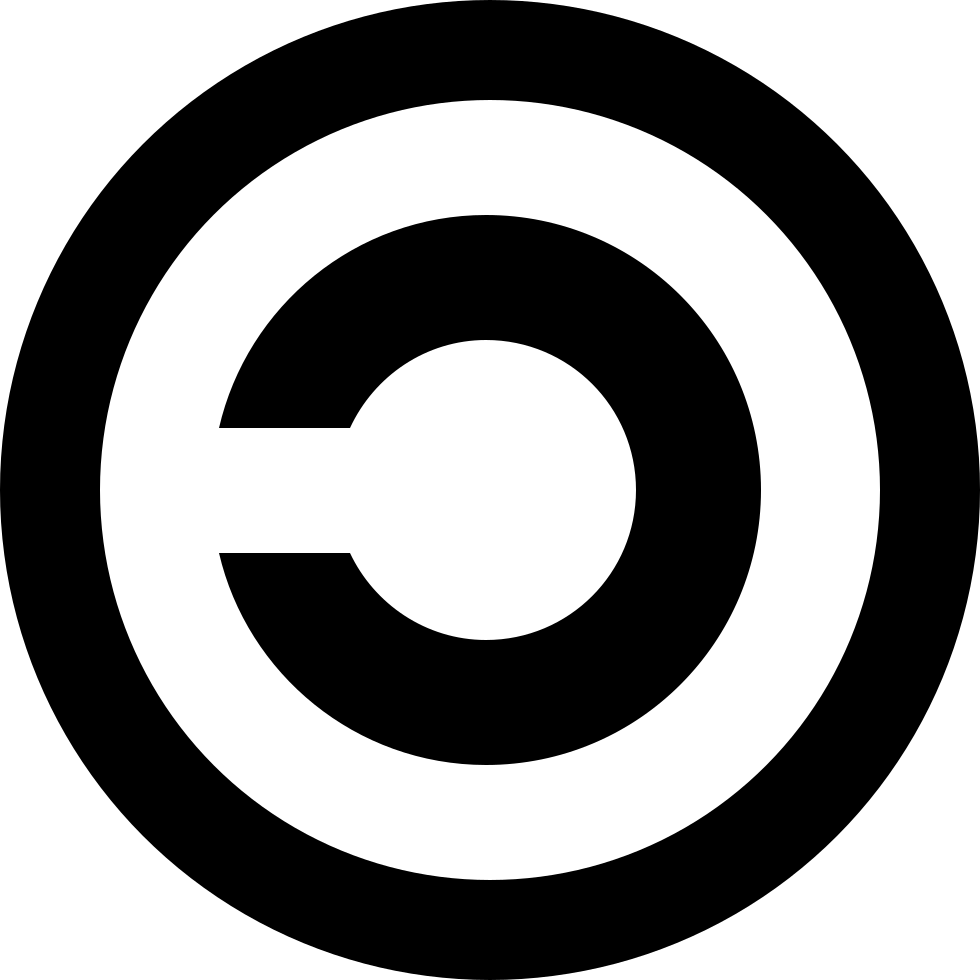
\includegraphics[width=1cm]{Copyleft.svg}
        \else
            
\includegraphics[width=1cm]{Copyleft.eps}
        \fi

Copyright (c) 2011-2012  Laurent Claessens,

Permission is granted to copy, distribute and/or modify this document under the terms of the \href{http://www.gnu.org/licenses/fdl-1.3.html}{GNU Free Documentation License}, Version 1.3 or any later version published by the Free Software Foundation; with no Invariant Sections, no Front-Cover Texts, and no Back-Cover Texts. A copy of the license is included in the section entitled ``GNU Free Documentation License''.

% Ajouter ici l'ISBN. Pour les révisions, mettre un nouvel ISBN et indiquer que c'est une révision.
% Pour l'ISBN:
% Copier tout dans un nouveau répertoire
% Créer une nouvelle branche git
% Coder en dur la date (càd enlever \today)
% Changer la licence vers non modifiable, copiable, et ajouter un lien vers la
%   version modifiable.

% http://www.bnf.fr/fr/professionnels/s_informer_obtenir_isbn/s.qu_est_ce_que_isbn.html

% TODO: écrire le README.txt

\end{center}

\clearpage



\tableofcontents

% This is part of Mes notes de mathématique
% Copyright (c) 2011-2012
%   Laurent Claessens
% See the file fdl-1.3.txt for copying conditions.

%+++++++++++++++++++++++++++++++++++++++++++++++++++++++++++++++++++++++++++++++++++++++++++++++++++++++++++++++++++++++++++
\section{Avertissement}
%+++++++++++++++++++++++++++++++++++++++++++++++++++++++++++++++++++++++++++++++++++++++++++++++++++++++++++++++++++++++++++

Ceci sont des notes «prises au vol» de certains de mes cours pour l'agrégation. Aucune garantie. Merci de me signaler toute faute ou remarque. En particulier je serais content que quelqu'un me donne un avis sur le points suivants :
\begin{enumerate}
    \item
        L'énoncé et la démonstration de la proposition \ref{PropNsLqWb}.
    \item
        Où trouver une preuve de la proposition \ref{PropKZDqTR} sur le supplémentaire topologique ?
    \item
        La preuve du théorème \ref{ThoJsBKir}.
    \item
        La preuve du lemme \ref{LemjXywjH}.
    \item
        La preuve du théorème de Fredholm \ref{ThoagJPZJ}.
    \item
        La preuve du lemme \ref{LemooynkH}.
    \item
        La partie «unicité» du théorème \ref{ThokUUlgU}.
    \item
        La preuve de la proposition \ref{PropRZCKeO}.
    \item
        L'inversion entre la somme et l'intégrale de l'équation \eqref{EqXSgZGw}.
    \item
        Si vous connaissez des exemples ou des contre-exemples intéressants à propos de quoi que ce soit, je suis toujours preneur.
\end{enumerate}

Une version avec ISBN de ce document est en préparation afin qu'il soit acceptable comme livre aux oraux de l'agrégation \ldots j'y travaille et on verra comment les choses vont évoluer.

%+++++++++++++++++++++++++++++++++++++++++++++++++++++++++++++++++++++++++++++++++++++++++++++++++++++++++++++++++++++++++++
\section{Auteurs, contributeurs et remerciements}
%+++++++++++++++++++++++++++++++++++++++++++++++++++++++++++++++++++++++++++++++++++++++++++++++++++++++++++++++++++++++++++

Le principal auteur et metteur en \LaTeX\ de ce document est votre serviteur, Laurent Claessens.

Les personnes qui ont du code \LaTeX\ dans ce document :
\begin{enumerate}
    \item
        Nicolas Richard et Ivik Swan pour les parties des exercices et rappels de calcul différentiel et intégral (Université libre de Bruxelles, 2003-2004) qui leur reviennent.
    \item
        Pierre Bieliavsky pour les énoncés d'analyse numérique (MAT1151 à Louvain la Neuve 2009-2010)
    \item
        Jonathan Di Cosmo pour certaines corrections de MAT1151
\end{enumerate}

Autres sources et remerciements :
\begin{enumerate}
    \item
        Tous les contributeurs du wikipédia francophone (et aussi un peu l'anglophone) doivent être remerciés. J'en ai pompé des quantités astronomiques; des articles utilisés sont cités à divers endroits du texte, mais ce n'est absolument pas exhaustif. Il n'y a à peu près pas un résultat important de ces notes dont je n'aie pas lu la page Wikipédia, et souvent plusieurs pages connexes.
    \item
        Des centaines de profs qui ont mis leurs polys sur internet. Des dizaines d'entre eux (et entre elles) ont des sites dédiés à l'agrégation. Ils sont cités en bibliographie aux endroits où ils sont utilisés. Merci à toutes et à tous d'avoir codé et publié.
    \item
        Le forum usenet de math, en particulier pour la construction des corps fini dans la fil «Vérifier qu'un polynôme est primitif» initié le 20 décembre 2011.
\end{enumerate}

%+++++++++++++++++++++++++++++++++++++++++++++++++++++++++++++++++++++++++++++++++++++++++++++++++++++++++++++++++++++++++++
					\section*{Ces notes sont les vôtres !}
%+++++++++++++++++++++++++++++++++++++++++++++++++++++++++++++++++++++++++++++++++++++++++++++++++++++++++++++++++++++++++


Il y a encore certainement des erreurs, des fautes de frappe et des choses pas claires. Je compte sur vous (oui : toi !) pour me signaler toute imperfection (y compris d'orthographe).

Plus vous signalez de fautes, meilleure sera la qualité du texte, et plus les étudiants de l'année prochaine vous seront reconnaissants.

%Tiens, tant que j'y suis je vous demanderais de penser à la quantité d'argent que vous auriez dû dépenser pour obtenir un texte tel que celui-ci chez un éditeur «classique» qui vous interdirait la photocopie et la redistribution. Maintenant que vous y avez pensé, je vous donnerais bien mon numéro de compte, mais non. J'ai tapé ce texte sur mes heures de travail à l'université; j'ai donc déjà été payé par les contribuables belges et français.

%+++++++++++++++++++++++++++++++++++++++++++++++++++++++++++++++++++++++++++++++++++++++++++++++++++++++++++++++++++++++++++
\section{Contre Moodle, Icampus, Claroline, et autres «plateformes de travail collaboratif»}
%+++++++++++++++++++++++++++++++++++++++++++++++++++++++++++++++++++++++++++++++++++++++++++++++++++++++++++++++++++++++++++

Ces notes ne sont pas destinées à être publiées sur des plateformes telles que Moodle, Icampus ou autres Clarolines. Pourquoi ? parce que la licence FDL l'interdit implicitement en demandant de publier sur des sites \emph{ouverts}.

L'internet est un système décentralisé et ouvert : tout le monde peut s'y connecter, y publier et y lire. C'est pour l'instant la meilleure solution technique inventée par l'humanité pour la diffusion d'information. Des sites comme \href{http://gitorious.org}{gitorious} ou \href{http://wikipedia.org}{wikipedia} sont de \emph{vrais} système de travail collaboratif.

Les plateformes soi-disant collaboratives comme Moodle en sont la négation. L'essentiel de ce qu'apporte Moodle par rapport à un vrai site internet n'est absolument pas la possibilité de partager des information (ça on peut le faire via internet depuis des décennies), mais bien de \emph{restreindre} l'accès à l'information via un système de mot de passe.

Lorsqu'un moine copiste du onzième siècle mettait un manuscrit dans sa bibliothèque, le document était immédiatement consultable par une centaine de moines, et (quitte à faire le déplacement) par des milliers d'érudits. Un document posté sur Moodle touche une dizaine de personnes. Utiliser Moodle pour partager ses documents est donc une régression non pas par rapport à l'internet d'il y a vingt ans, non pas par rapport à l'imprimerie d'il y a cinq siècles, mais bien par rapport aux bibliothèques d'abbayes d'il y a mille ans !

Lorsqu'on parle de science, qu'on veut y apporter un document, une question ou une réponse, un minimum d'honnête intellectuelle, d'éthique du partage de savoir (sans laquelle la science n'existe pas) et peut être aussi de courage, est de parler publiquement. Se cacher derrière un mot de passe et ne permettre l'accès au savoir qu'à ses seuls amis triés sur le volet est une négation de l'esprit scientifique; Moodle est une version dégénérée, une maladie de l'internet.

La faute fondamentale qui fait utiliser Moodle pour partager des documents de mathématique est la perte de notion entre le privé et le public ainsi que la paresse qui consiste à vouloir intégrer tous les outils dans une même interface, voire utiliser les mêmes outils pour effectuer des tâches différentes. Lorsqu'on pose une question de math, c'est essentiellement public; lorsqu'on pose une question d'organisation d'un cours, c'est privé. Ce sont deux activités totalement différentes qui nécessitent deux types d'outils différents. Dans le premier cas, l'outil adapté est internet, dans le deuxième cas, l'outil adapté est Moodle. Vouloir utiliser la même interface pour les deux est n'avoir fondamentalement pas compris le sens de l'internet et son utilité en tant que «outil de l'information».

{\tiny Cela dit c'est pratique pour discuter des horaires des cours ou s'échanger des informations pratiques qui n'ont pas à être publiques.}

%+++++++++++++++++++++++++++++++++++++++++++++++++++++++++++++++++++++++++++++++++++++++++++++++++++++++++++++++++++++++++++
\section{Instructions pour les examens et interrogations}
%+++++++++++++++++++++++++++++++++++++++++++++++++++++++++++++++++++++++++++++++++++++++++++++++++++++++++++++++++++++++++++

Ceci sont des conseils généraux que nous vous conseillons de suivre dans toutes les matières.
\begin{description}
    \item[numéroter] Numérotez clairement toutes les questions. Si votre réponse prend plus d'une page, écrivez «suite au verso», «suite à l'intercalaire \( n\)» etc. À l'endroit où la réponse continue, écrivez «question \( n\), suite».

    \item[vérifiez] Certaines erreurs sont faciles à détecter. Par exemple
        \begin{enumerate}
            \item
                les aires et volumes sont positifs;
            \item
                une intégrale \emph{définie} qui contient «\( dx\)» ne peut pas contenir de \( x\) dans la réponse;

            \item
                en physique et en chimie, les unités doivent être cohérentes : si la réponse est une énergie, vous devez avoir des joules (\unit{\square\metre\kilo\gram\per\square\second}).

        \end{enumerate}
    \item[votre nom] Écrivez votre nom et votre numéro de carte d'étudiant.

    \item[les faciles d'abord] Lisez d'abord toutes les questions avant de répondre. Commencez par les questions faciles.

    \item[justifier] Justifiez vos réponses. N'hésitez pas à écrire des phrases complètes : sujet, verbe, complément. N'abusez pas des symboles dont vous ignorez la signification :
        \begin{enumerate}
            \item
                «\( \Leftrightarrow\)» signifie «si et seulement si», et non «la suite de mon calcul»;
            \item

                «\( \nexists\)» signifie «il n'existe pas», et non «n'existe pas» ou «n'est pas défini».
        \end{enumerate}

    \item[ne pas passer en force] Si vous savez que votre réponse est fausse, mais vous ne savez pas la corriger, écrivez sur votre feuille «cette réponse est fausse pour telle raison, mais je ne sais pas comment corriger». Ne comptez pas sur une inattention du correcteur. En science, affirmer un fait que vous savez être faux s'appelle de la falsification; c'est déontologiquement inacceptable. De la même façon, si vous copiez sur votre voisin\footnote{Indépendamment que c'est sans doute interdit par le règlement; vérifiez avant.}, vous êtes priés de le citer : on ne s'approprie pas le travail d'autrui.

    \item[approximations numériques] Lorsque vous voulez écrire une approximation numérique, réfléchissez au sens de ce que vous allez écrire. En mathématique, ça n'a presque jamais de sens d'écrire une approximation parce que vous ne savez pas dans quel contexte votre calcul pourra être utilisé. Si vous laissez deux décimales à \( \pi\) pour calculer le volume d'eau dans votre piscine gonflable, ça fera l'affaire; si c'est pour calculer la masse du Higgs ou pour mettre un satellite autour de Mars, vous perdez plusieurs millions d'euros.

        En sciences naturelles (physique, chimie ou autres), vous pouvez donner des approximations numériques de façon circonstanciée. Demandez à votre prof de labo.

    \item[orthographe] Sans être obligatoire, ça ne fait jamais de mal. Surtout si le français est votre langue maternelle.
    \item[santé] Mangez des fruits et des légumes de saisons. Choisissez des producteurs locaux qui n'utilisent pas d'engrais synthétisés à base de pétrole. De toutes façons \href{http://www.energybulletin.net/node/51306}{vous n'avez pas le choix}.

\end{description}

%+++++++++++++++++++++++++++++++++++++++++++++++++++++++++++++++++++++++++++++++++++++++++++++++++++++++++++++++++++++++++++
\section{Propagande : utilisez un ordinateur !}
%+++++++++++++++++++++++++++++++++++++++++++++++++++++++++++++++++++++++++++++++++++++++++++++++++++++++++++++++++++++++++++

Si vous faites des exercices supplémentaires et que vous voulez des corrections, n'oubliez pas que vous avez un ordinateur à disposition. De nos jours, les ordinateurs sont capables de calculer à peu près tout ce qui se trouve dans vos cours de math\footnote{Avec une notable exception pour les limites à deux variables.}.

D'ailleurs, je te rappelle que nous sommes est déjà largement dans le vingt et unième siècle et que tu te destines à une carrière professionnelle dans laquelle tu auras des calculs à faire; si tu n'es pas encore capable d'utiliser un ordinateur pour faire ces calculs, il est temps de combler cette lacune.

%---------------------------------------------------------------------------------------------------------------------------
\subsection{Lancez-vous dans Sage}
%---------------------------------------------------------------------------------------------------------------------------

Le logiciel que je vous propose est \href{http://www.sagemath.org}{Sage}. Pour l'utiliser, il n'est même pas nécessaire de l'installer sur votre ordinateur~: il tourne en ligne, directement dans votre navigateur.

\begin{enumerate}

	\item
		Aller sur \href{http://www.sagenb.org}{http://www.sagenb.org}
	\item
		Créer un compte
	\item
		Créer des feuilles de calcul et amusez-vous !!

\end{enumerate}

Il y a beaucoup de \href{http://lmgtfy.com/?q=sage+documentation}{documentation} sur le \href{http://www.sagemath.org}{site officiel}\footnote{\href{http://www.sagemath.org}{http://www.sagemath.org}}.

Si vous comptez utiliser régulièrement ce logiciel, je vous recommande \emph{chaudement} de \href{http://mirror.switch.ch/mirror/sagemath/index.html}{l'installer} sur votre ordinateur. Ce logiciel étant distribué sous licence GPL, vous ne devez ni payer ni vous procurer de codes.

%---------------------------------------------------------------------------------------------------------------------------
\subsection{Exemples de ce que Sage peut faire pour vous}
%---------------------------------------------------------------------------------------------------------------------------

Voici une liste absolument pas exhaustive de ce que Sage peut faire pour vous, avec des exemples. 
\begin{enumerate}

	\item
		Calculer des limites de fonctions, voir l'exercice \ref{exoINGE11140028},

	\item
		D'autres limites et tracer des fonctions, voir l'exercice \ref{exoINGE11140031}.
	\item
		Calculer des dérivées, voir exercice \ref{exo0013}.
	\item
		Calculer des dérivées partielles de fonctions à plusieurs variables, voir exercice \ref{exoFoncDeuxVar0002}.
	\item
		Calculer des primitives, voir certains exercices \ref{exo0017}
	\item

		Résoudre des systèmes d'équations linéaires. Lire \href{http://www.sagemath.org/doc/constructions/linear_algebra.html#solving-systems-of-linear-equations}{la documentation} est ce qui fait la différence entre l'être humain et le non scientifique. Voir les exercices  \ref{exoINGE1121La0016} et \ref{exoINGE1121La0010}.

	\item
		Tout savoir d'une forme quadratique, voir exercice \ref{exoINGE1121La0018}.
	\item
		Calculer la matrice Hessienne de fonctions à deux variables, déterminer les points critiques, déterminer le genre de la matrice Hessienne aux points critiques et écrire extrema de la fonctions (sous réserve d'être capable de résoudre certaines équations), voir les exercices \ref{exoFoncDeuxVar0029} et \ref{exoFoncDeuxVar0028}.
	\item
		Lorsqu'il y a une infinité de solutions, Sage vous l'indique avec des paramètres (ne fonctionne hélas pas avec les fonctions trigonométriques), voir l'exercice \ref{exoDerrivePartielle-0007}.


	\item
		Calculer des dérivées symboliquement, voir exercice \ref{exoDerive-0002}.
	\item
		Calculer des approximations numériques comme dans l'exercice \ref{exoOutilsMath-0028}.
    \item
        Calculer dans un corps de polynômes modulo comme \( \eF_p[X]/P\) où \( P\) est un polynôme à coefficients dans \( \eF_p\). Voir l'exemple \ref{ExemWUdrcs}.
	\item
        Tracer des courbes en trois dimensions, voir exemple \ref{ExempleTroisDxxyy}. Notez que pour cela vous devez installer aussi le logiciel Jmol. Pour Ubuntu\footnote{Pour les autres, je ne sais pas, mais je laisserai jouer l' adage «Windows c'est facile». Quant aux utilisateurs d'OS «alternatifs» comme Hurd ou BSD ben heu \ldots} c'est dans le paquet \info{icedtea6-plugin}.
\end{enumerate}

Sage peut toutefois vous induire en erreur si vous n'y prenez pas garde parce qu'il sait des choses en mathématique que vous ne savez pas. Par conséquent il peut parfois vous donner des réponses (mathématiquement exactes) auxquelles vous ne vous attendez pas. Voir page \ref{PgpXBuBh}.

%+++++++++++++++++++++++++++++++++++++++++++++++++++++++++++++++++++++++++++++++++++++++++++++++++++++++++++++++++++++++++++
%\section{Propagande : n'utilisez pas votre calculatrice}
%+++++++++++++++++++++++++++++++++++++++++++++++++++++++++++++++++++++++++++++++++++++++++++++++++++++++++++++++++++++++++++

%D'abord, l'expérience montre que la majorité des fois qu'un étudiant sort sa calculatrice, c'est pour faire un calcul inutile, et le plus souvent la calculatrice fournit un résultat faux. Étant en 2012, vous ne devriez pas vous contenter de vos calculatrices qui coûtent un os, qui n'ont pas de puissance de calcul, qui ont une définition d'écran ridicule et en noir et blanc. Remarquez que votre GSM (et a forciori vos minis trucs qui se connectent a internet) sont considérablement plus puissants que ces vieilleries; ils ont un meilleur écran.


\chapter{Théorie de la mesure et variable aléatoires}
% This is part of Mes notes de mathématique
% Copyright (c) 2011-2012
%   Laurent Claessens
% See the file fdl-1.3.txt for copying conditions.


\section{Séries}
\label{secseries}

\subsection{Rappels et définitions}
La notion de série formalise le concept de somme infinie. L'absence de
certaines propriétés de ces objets (problèmes de commutativité et même
d'associativité) incitent à la prudence et montrent à quel point une
définition précise est importante.

Soit ${(a_k)}_{k \geq k_0}$ une suite réelle. La \defe{série} de terme
général $(a_k)${série}, notée
\begin{math}
  \sum_{i=k_0}^\infty a_i,
\end{math}
est la suite ${(s_n)}_{n \geq k_0}$ dont les termes sont donnés par
\begin{equation*}
  s_n \pardef \sum_{i=k_0}^k a_i
\end{equation*}
et sont appelés les \defe{sommes partielles}{somme!partielle} de la série.

La série $\sum_{i=k_0}^\infty a_i$ \defe{converge}{série!convergence} si la suite $(s_n)$
converge vers un réel $s$. Sa limite est appelée la \defe{somme de la
série}{série!somme} et on note
\begin{equation}		\label{EqDefSommeLim}
  \sum_{i=k_0}^\infty a_i = \lim_{n\to\infty}\sum_{i=k_0}^na_i.
\end{equation}
Si la série ne converge pas, elle \defe{diverge}{série!divergence} et peut alors avoir
une limite infinie (uniquement si le terme général est réel, on note
alors $+\infty$ ou $-\infty$ sa limite) ou pas de limite.  La série
$\sum_{i=k_0}^\infty a_i$ \defe{converge absolument}{convergence!absolue} si la série
$\sum_{i=k_0}^\infty \abs{a_i}$ converge.

\begin{proposition}\label{propnseries_propdebase}
Les principales propriétés de la somme définie par la limite \eqref{EqDefSommeLim} sont
  \begin{enumerate}
  \item Si une série converge absolument, alors elle converge
    (simplement).
  \item Si la série est à termes positifs --c'est-à-dire pour tout
    indice $k$, $a_k \in \eR$ et $a_k \geq 0$-- il n'y a aucune
    différence entre convergence absolue et convergence simple.
  \item\label{point3-seriepropdebase} Si une série converge, son terme général doit tendre vers $0$.
\item 
Si la série converge alors la somme est associative
\item
Si la série converge absolument, alors la somme est commutative.
  \end{enumerate}
\end{proposition}

\begin{remark}Vue comme somme infinie, l'associativité et la
  commutativité dans une série sont perdues. Néanmoins, il subsiste
  que
  \begin{enumerate}
  \item si la série converge, on peut regrouper ses termes sans
    modifier la convergence ni la somme (associativité),
  \item si la série converge absolument, on peut modifier l'ordre des
    termes sans modifier la convergence ni la somme (commutativité).
  \end{enumerate}
\end{remark}

\begin{example}\label{exemplesseries}
\begin{enumerate}

\item
    La \defe{série harmonique}{série!harmonique} est
\begin{equation}
\sum_{i=1}^\infty \frac1i
\end{equation}
et diverge (possède une limite $+\infty$).

\item
    La \defe{série géométrique}{série!géométrique} de raison $q \in \eC$ est
\begin{equation}
\sum_{i=0}^\infty q^i.
\end{equation}
Étudions la somme partielle \( S_N=1+q+q^2+\ldots +q^{n}\). Nous avons évidemment $S_N-zS_N=1-q^{N+1}$ et donc
\begin{equation}
    S_N=\sum_{n=0}^N=\frac{ 1-q^{N+1} }{ 1-q }.
\end{equation}
La limite \( \lim_{N\to \infty} S_N\) existe si et seulement si \( | q |\leq 1\) et dans ce cas nous avons
\begin{equation}
    \sum_{n=1}^{\infty}q^n=\frac{ 1 }{ 1-z }.
\end{equation}
La convergence est absolue.

\item
Pour $\alpha \in \RR$, la série de Riemann (ou Dirichlet)
\begin{equation}		\label{EqSerRiem}
\sum_{i=1}^\infty \frac1{i^\alpha}
\end{equation}
converge (absolument, puisque réelle et positive) si et seulement
si $\alpha > 1$, et diverge sinon.
\end{enumerate}
\end{example}

\subsection{Critères de convergence absolue}

  Étant donné le terme général d'une série, il est souvent --dans les cas qui nous intéressent-- difficile de déterminer la somme de la série. L'exemple de la série géométrique est particulier, puisqu'on connait une formule pour chaque somme partielle, mais pour l'exemple des séries de Riemann il n'y a aucune formule simple pour un $\alpha$ général. D'où l'intérêt d'avoir des critères de convergence ne nécessitant aucune connaissance de l'éventuelle limite de la série.

\subsubsection{Critère de comparaison} 

Soient $\sum_i a_i$ et $\sum_j
b_j$ deux séries à termes positifs vérifiant
\begin{equation*}
  0 \leq a_i \leq b_i
\end{equation*}
alors
\begin{enumerate}
\item si $\sum_i a_i$ diverge, alors $\sum_j b_j$ diverge,
\item si $\sum_j b_j$ converge, alors $\sum_i a_i$ converge
  (absolument).
\end{enumerate}

\subsubsection{Critère d'équivalence}
\label{PgCritEquiv}

\begin{proposition}[\cite{TrenchRealAnalisys}]
 Soient $\sum_i a_i$ et $\sum_j b_j$ deux séries à termes positifs. Supposons l'existence de la limite (éventuellement infinie) suivante
\begin{equation}
  \limite i \infty \frac{a_i}{b_i} = \alpha \in \RR \text{ ou $\alpha =
    \infty$.}
\end{equation}
Dans ce cas, nous avons
\begin{enumerate}
\item si $\alpha \neq 0$ et $\alpha\neq \infty$, alors
  \begin{equation}
    \sum_i a_i \text{~converge} \ssi \sum_j b_j\text{~converge,}
  \end{equation}
\item si $\alpha = 0$ et $\sum_j b_j$ converge, alors $\sum_i a_i$
  converge (absolument),
\item si $\alpha = +\infty$ et $\sum_j b_j$ diverge, alors $\sum_i
  a_i$ diverge.
\end{enumerate}
\end{proposition}

\begin{proof}
\begin{enumerate}
	\item
		Le fait que la suite $a_n/b_n$ converge vers $\alpha$ signifie que tant sa limite supérieure que sa limite inférieure convergent vers $\alpha$. En particulier la suite $\frac{ a_n }{ b_n }$ est bornée vers le haut et vers le bas. À partir d'un certain rang $N$, il existe $M$ tel que 
		\begin{equation}
			\frac{ a_n }{ b_n }<M
		\end{equation}
		et il existe $m$ tel que
		\begin{equation}
			\frac{ a_n }{ b_n }>m.
		\end{equation}
		Nous avons donc $a_n<Mb_n$ et $a_n>mb_n$. La série de $(a_n)$ converge donc si et seulement si la série de $(b_n)$ converge.
	\item
		Si $\alpha=0$, cela signifie que pour tout $\epsilon$, il existe un rang tel que $\frac{ a_n }{ b_n }<\epsilon$, et donc tel que $a_n<\epsilon b_k$. La suite de $(a_i)$ converge donc dès que la suite de $(b_i)$ converge.
	\item
		Pour tout $M$, il existe un rang dans la suite à partir duquel on a $\frac{ a_i }{ b_i }>M$, et donc $a_k>Mb_k$. Si la série de $(b_k)$ diverge, la série de $(a_k)$ doit également diverger.
\end{enumerate}
\end{proof}

\subsubsection{Critère du quotient}

\begin{proposition}[\cite{KeislerElemCalculus}]
    Soit $\sum_i a_i$ une série. Supposons l'existence de la limite (éventuellement infinie) suivante
    \begin{equation}
      \limite i \infty \abs{\frac{a_{i+1}}{a_i}} = L\in \RR \text{ ou $L =
        \infty$.}
    \end{equation}
    Alors
    \begin{enumerate}
    \item si $L < 1$, la série converge absolument,
    \item si $L > 1$, la série diverge,
    \item si $L = 1$ le critère échoue : il existe des exemple de convergence et des exemples de divergence.
    \end{enumerate}
\end{proposition}

\begin{proof}
\begin{enumerate}
	\item
		Soit $b$ tel que $L<b<1$. À partir d'un certain rang $K$, on a $\left| \frac{ a_{i+1} }{ a_i } \right| <b$. En particulier,
		\begin{equation}
			| a_{K+1} |<b| a_K |,
		\end{equation}
		et pour $a_{K+2}$ nous avons
		\begin{equation}
			| a_{K+2} |<b| a_{K+1} |<b^2| a_K |.
		\end{equation}
		Au final,
		\begin{equation}
			| a_{K+n} |<b^n| a_K |.
		\end{equation}
		Étant donné que la série $\sum_{n\geq K}b^n$ converge (parce que $b<1$), la queue de suite $\sum_{i\geq K}a_i$ converge, et par conséquent la suite au complet converge.
	\item
		Si $L>1$, on a
		\begin{equation}
			| a_K |<| a_{K+1} |<| a_{K+2} |<\ldots
		\end{equation}
		Il est donc impossible que la suite $(a_i)$ converge vers zéro. La série ne peut donc pas converger.
	\item
		Par exemple la suite harmonique $a_n=\frac{1}{ n }$ vérifie $L=1$, mais la série ne converge pas. Par contre, la suite $a_n=\frac{ 1 }{ n^2 }$ vérifie aussi le critère avec $L=1$ tandis que la série $\sum_n\frac{1}{ n^2 }$ converge.
\end{enumerate}
\end{proof}

\subsubsection{Critère de la racine}

\begin{proposition}[\cite{TrenchRealAnalisys}]
    Soit $\sum_i a_i$ une série, et considérons
    \begin{equation*}
      \limsup_{i \rightarrow \infty} \sqrt[i]{\abs{a_i}} = L \in \RR
      \text{ ou $L =
        \infty$.}
    \end{equation*}
    Alors
    \begin{enumerate}
    \item si $L < 1$, la série converge absolument,
    \item si $L> 1$, la série diverge,
    \item si $L = 1$ le critère échoue.
    \end{enumerate}
\end{proposition}

\begin{proof}
    \begin{enumerate}
        \item
            Si $L<1$, il existe un $r\in \mathopen] 0 , 1 \mathclose[$ tel que $| a_n |^{1/n}<r$ pour les grands $n$. Dans ce cas, $| a_n |<r^{n}$, et la série converge absolument parce que la série $\sum_nr^n$ converge du fait que $r<1$.
        \item
            Si $L>1$, il existe un $r>1$ tel que $| a_n |^{1/n}>r>1$. Cela fait que $| a_n |$ prend des valeurs plus grandes que $n$ pour une infinité de termes. Le terme général $a_n$ ne peut donc pas être une suite convergente. Par conséquent la suite diverge au sens où elle ne converge pas.

    \end{enumerate}
\end{proof}

%---------------------------------------------------------------------------------------------------------------------------
\subsection{Critères de convergence simple}
%---------------------------------------------------------------------------------------------------------------------------

Les critères de comparaison, d'équivalence, du quotient et de la racine sont des critères de convergence absolue. Pour conclure à une convergence simple qui n'est pas une convergence absolue, le critère d'Abel sera notre outil principal.  

\subsubsection{Critère d'Abel}

\begin{proposition}[Critère d'Abel]
    Soit la série $\sum_i c_iz_i$ avec
    \begin{enumerate}
        \item $(c_i)$ est une suite réelle décroissante qui tend vers zéro,
        \item $(z_i)$ est une suite dans $\eC$ dont la suite des sommes partielles est bornée dans $\eC$, c'est à dire qu'il existe un $M>0$ tel que pour tout $n$,
        \begin{equation}
            \left| \sum_{i=1}^nz_i \right| \leq M.
        \end{equation}
        Alors la série $\sum_ic_iz_i$ est convergente.
    \end{enumerate}
\end{proposition}
Remarquons que ce critère ne donne pas de convergence absolue.

\begin{corollary}[Critère des séries alternées]\index{critère!série alternée}       \label{CoreMjIfw}
    Si \( (a_n)\) est une suite décroissante à limite nulle, alors la série
  \begin{equation}
    \sum_{n=0}^\infty {(-1)}^n a_n
  \end{equation}
  converge simplement.
\end{corollary}

%+++++++++++++++++++++++++++++++++++++++++++++++++++++++++++++++++++++++++++++++++++++++++++++++++++++++++++++++++++++++++++
					\section{Développements de Taylor et Maclaurin}
%+++++++++++++++++++++++++++++++++++++++++++++++++++++++++++++++++++++++++++++++++++++++++++++++++++++++++++++++++++++++++++

%---------------------------------------------------------------------------------------------------------------------------
\subsection{Fonctions «petit o» }
%---------------------------------------------------------------------------------------------------------------------------

Nous voulons formaliser l'idée d'une fonction qui tend vers zéro \og plus vite\fg{} qu'une autre. Nous disons que $f\in o\big(\varphi(x)\big)$ si
\begin{equation}
	\lim_{x\to 0} \frac{ f(x) }{ \varphi(x) }=0.
\end{equation}
En particulier, nous disons que $f\in o(x)$ lorsque $\lim_{x\to 0} f(x)/x=0$.

%---------------------------------------------------------------------------------------------------------------------------
\subsection{Formule et reste}
%---------------------------------------------------------------------------------------------------------------------------

\begin{proposition}		\label{PropDevTaylorPol}
    Soient $f\colon I\subset\eR\to \eR$ et $a\in\Int(I)$. Soit un entier $k\geq 1$. Si $f$ est $k$ fois dérivable en $a$, alors il existe un et un seul polynôme $P$ de degré $\leq k$ tel que
    \begin{equation}
        f(x)-P(x-a)\in o\big( | x-a |^k \big)
    \end{equation}
    lorsque $x\to a$, $x\neq a$. Ce polynôme  est donné par
    \begin{equation}
        P(h)=f(a)+f'(a)h+\frac{ f''(a) }{ 2! }h^2+\ldots+\frac{ f^{(k)}(a) }{ k! }h^k.
    \end{equation}
    Notons encore deux façons alternatives d'écrire le résultat. Si \( f\in C^k\) il existe une fonction \( \alpha\) telle que \( \lim_{t\to 0} \alpha(t)=0\) et
    \begin{equation}
        f(x)=\sum_{n=0}^k\frac{ f^{(n)}(a) }{ n! }(x-a)^n+(x-a)^n\alpha(x-a).
    \end{equation}
    Si \( f\in C^{k+1}\) alors
    \begin{equation}        \label{EquQtpoN}
        f(x)=\sum_{n=0}^k\frac{ f^{(n)}(a) }{ n! }(x-a)^n+(x-a)^{n+1}\xi(x-a)
    \end{equation}
    où \( \xi\) est une fonction telle que \( \xi(t)\) tend vers une constante lorsque \( t\to 0\).
\end{proposition}

La proposition suivant donne une intéressante façon de trouver le reste d'un développement de Taylor.
\begin{proposition}		\label{PropResteTaylorc}
Soient $I$, un intervalle dans $\eR$ et $f\colon I\to \eR$ une fonction de classe $C^k$ sur $I$ telle que $f^{(k+1)}$ existe sur $I$. Soient $a\in\Int(I)$ et $x\in I$. Alors il existe $c$ strictement compris entre $x$ et $a$ tel que 
\begin{equation}
	R_{f,a,k}(x)=\frac{ f^{(k+1)}(c) }{ (k+1)! }(x-a)^{k+1}.
\end{equation}
\end{proposition}

%---------------------------------------------------------------------------------------------------------------------------
					\subsection{Exemple : un calcul heuristique de limite}
%---------------------------------------------------------------------------------------------------------------------------
\label{SubSecCalcLimHeuris}

Au cours de la résolution de l'exercice \ref{exoEqsDiff0002}\ref{ItemfEqsDiff00002}, nous devons calculer la limite suivante :
\begin{equation}
	\lim_{x\to 0} \frac{  e^{-2\cos(x)+2}\sin(x) }{ \sqrt{ e^{2\cos(x)+2}}-1 }.
\end{equation}
La stratégie que nous allons suivre pour calculer cette limite est de développer certaines parties de l'expression en série de Taylor, afin de simplifier l'expression. La première chose à faire est de remplacer $ e^{y(x)}$ par $1+y(x)$ lorsque $y(x)\to 0$. La limite devient
\begin{equation}
	\lim_{x\to 0} \frac{ \big( -2\cos(x)+3 \big)\sin(x) }{ \sqrt{-2\cos(x)+2} }.
\end{equation}
Nous allons maintenant remplacer $\cos(x)$ par $1$ au numérateur et par $1-x^2/2$ au dénominateur. Pourquoi ? Parce que le cosinus du dénominateur est dans une racine, donc nous nous attendons à ce que le terme de degré deux du cosinus donne un degré un en dehors de la racine, alors que du degré un est exactement ce que nous avons au numérateur : le développement du sinus commence par $x$.

Nous calculons donc
\begin{equation}
	\begin{aligned}[]
		\lim_{x\to 0} \frac{ \sin(x) }{ \sqrt{-2\left( 1-\frac{ x^2 }{ 2 } \right)+2} }=\lim_{x\to 0} \frac{ \sin(x) }{ x }=1.
	\end{aligned}
\end{equation}
Tout ceci n'est évidement pas très rigoureux, mais en principe vous avez tous les éléments en main pour justifier les étapes.

%+++++++++++++++++++++++++++++++++++++++++++++++++++++++++++++++++++++++++++++++++++++++++++++++++++++++++++++++++++++++++++
\section{Théorie de la mesure}
%+++++++++++++++++++++++++++++++++++++++++++++++++++++++++++++++++++++++++++++++++++++++++++++++++++++++++++++++++++++++++++

Pour la théorie de la mesure, voir entre autres \cite{FubiniBMauray,ProbaDanielLi}.

%---------------------------------------------------------------------------------------------------------------------------
\subsection{Espaces mesurables et mesurés}
%---------------------------------------------------------------------------------------------------------------------------

\begin{definition}
    Si \( \Omega\) est un ensemble, un ensemble \( \tribA\) de sous-ensembles de \( \Omega\) est une \defe{tribu}{tribu} si
    \begin{enumerate}
        \item
            \( \Omega\in\tribA\);
        \item
            \( \complement A\in A\) pour tout \( A\in\tribA\);
        \item
            si \( (A_i)_{i\in I}\) est un ensemble au plus dénombrable d'éléments de \( \tribA\), alors \( \sup_{n\geq 1}A_n=\bigcup_{i\in I}A_i\in\tribA\).
    \end{enumerate}
    Le couple \( (\Omega,\tribA)\) est alors un \defe{espace mesuré}{espace!mesuré}.
\end{definition}

\begin{lemma}
    Une tribu est stable par intersections au plus dénombrables.
\end{lemma}

\begin{proof}
    Soit \( (A_i)_{i\in I}\) une famille au plus dénombrable d'éléments de la tribu \( \tribA\). Nous devons prouver que \( \bigcap_{i\in I}A_i\) est également un élément de \( \tribA\). Pour cela nous passons au complémentaire :
    \begin{equation}
        \complement\left( \bigcap_{i\in I}A_i \right)=\bigcup_{i\in I}\complement A_i.
    \end{equation}
    La définition d'une tribu implique que le membre de droite est un élément de la tribu. Par stabilité d'une tribu par complémentaire, l'ensemble \( \bigcap_{i\in I}A_i\) est également un élément de la tribu.
\end{proof}

La tribu que nous utiliserons toujours dans \( \eR^d\) est la tribu des \defe{boréliens}{boréliens}, notée \( \Borelien(\eR^d)\), qui est la tribu engendrée par les ouverts de \( \eR^d\). Une fonction \( f\colon (\Omega,\tribA)\to (\eR^d,\Borelien(\eR^d))\) est \defe{borélienne}{borélienne} si pour tout \( \mO\in\Borelien\), \( f^{-1}(\mO)\in\tribA\).

\begin{definition}
    Une \defe{\wikipedia{en}{Measure_space}{mesure}}{mesure} sur l'espace mesurable \( (\Omega,\tribA)\) est une application \( \mu\colon \tribA\to \eR\cup\{ \infty \}\) telle que
    \begin{enumerate}
        \item
            \( \mu(A)\geq 0\) pour tout \( A\in\tribA\);
        \item
            \( \mu(\emptyset)=0\);
        \item
            \( \mu\left( \bigcup_{i=0}^{\infty}A_i\right)=\sum_{i=0}^{\infty}\mu(A_i)\) si les \( A_i\) sont des éléments de \( \tribA\) deux à deux disjoints.
    \end{enumerate}
    Une mesure est \defe{\( \sigma\)-finie}{mesure!$\sigma$-finie} si il existe une suite croissante (pour l'inclusion) d'éléments \( (E_n)_{n\in\eN}\) de la tribu, tous de mesure finie et tels que \( \Omega=\bigcup_{n\in \eN}E_n\). Si la mesure est $\sigma$-finie, nous disons que l'espace \( (\Omega,\tribA,\mu)\) est un espace mesuré $\sigma$-fini.
\end{definition}

\begin{definition}
    Une application entre espace mesurés
    \begin{equation}
        f\colon (\Omega,\tribA)\to (\Omega',\tribA')
    \end{equation}
    est \defe{mesurable}{mesurable!application} si pour tout \( B\in\tribA'\), l'ensemble \( f^{-1}(B)\) est dans \( \tribA\).
\end{definition}

Si \( \mu\) est une mesure sur \( \eR^d\), une fonction \( f\colon \eR^d\to \eR\) est une \defe{densité}{densité d'une mesure} si pour tout \( A\subset\eR^d\) nous avons
\begin{equation}
    \mu(A)=\int_Af(x)dx
\end{equation}
où \( dx\) est la mesure de Lebesgue.

%---------------------------------------------------------------------------------------------------------------------------
\subsection{Mesure produit}
%---------------------------------------------------------------------------------------------------------------------------

\begin{definition}      \label{DefTribProfGfYTuR}
    Si \( \tribA\) et \( \tribB\) sont deux tribus sur deux ensembles \( \Omega_1\) et \( \Omega_2\), nous définissons la \defe{tribu produit}{tribu!produit} \( \tribA\otimes\tribB\) comme étant la tribu engendrée par 
    \begin{equation}
        \{ A\times B\tq A\in\tribA,B\in\tribB \}.
    \end{equation}
\end{definition}

\begin{theorem}\index{mesure!produit}
    Soient \( \mu_i\) des mesures $\sigma$-finies sur \( (\Omega_i,\tribA_i)\) (\( i=1,2\)). Il existe une et une seule mesure, notée \( \mu_1\otimes \mu_2\), sur \( (\Omega_1\times\Omega_2,\tribA_1\otimes\tribA_2)\) telle que
    \begin{equation}
        (\mu_1\otimes\mu_2)(A_1\times A_2)=\mu_1(A_1)\mu_2(A_2)
    \end{equation}
    pour tout \( A_1\in \tribA_1\) et \( A_2\in\tribA_2\).
\end{theorem}
Une preuve peut être trouvée dans \cite{FubiniBMauray}.

%---------------------------------------------------------------------------------------------------------------------------
\subsection{Intégrale par rapport à une mesure}
%---------------------------------------------------------------------------------------------------------------------------

Une fonction \( f\colon (\Omega,\tribA)\to (\Omega',\tribA')\) est \defe{mesurable}{mesurable!fonction} si 
\begin{equation}
    f^{-1}(E)\in\tribA
\end{equation}
pour tout \( E\in\tribA'\).


Une mesure \( \mu\) sur un espace mesurable \( (\Omega,\tribA)\) permet de définir une fonctionnelle linéaire sur l'ensemble des fonctions mesurables \( \Omega\to \eR\). Cette fonctionnelle linéaire est l'intégrale que nous allons définir à présent.

D'abord nous considérons les fonction \defe{simples}{simple!fonction}\index{fonction!simple}, c'est à dire les fonctions de la forme
\begin{equation}
    f=\sum_{i=1}^Na_i\caract_{E_i}
\end{equation}
où \( a_i\in\eR\) tandis que les \( E_i\) sont des ensembles \( \mu\)-mesurables. Si \( Y\in \tribA\) nous définissons
\begin{equation}
    \int_Yfd\mu=\sum_ia_i\mu(Y\cap E_i).
\end{equation}
Pour une fonction \( \mu\)-mesurable générale \( f\colon \Omega\to \mathopen[ 0 , \infty \mathclose]\) nous définissons l'intégrale de \( f\) sur \( Y\) par
\begin{equation}        \label{EqDefintYfdmu}
    \int_Yfd\mu=\sup\Big\{ \int_Yhd\mu\,\text{où \( h\) est une fonction simple et mesurable telle que \( 0\leq h\leq f\)} \Big\}.
\end{equation}
Maintenant nous définissons
\begin{equation}
    \mu(f)=\int_{\Omega}f
\end{equation}
si \( f\) est une fonction mesurable sur \( \Omega\).

\begin{remark}
    Dans \( \eR^d\), quasiment toutes les fonctions et ensembles sont mesurables. En effet la construction d'ensembles non mesurables demande obligatoirement l'utilisation de l'axiome du choix; de tels ensembles doivent être construits «exprès pour». Il y a très peu de chances pour que vous tombiez sur un ensemble non mesurable de \( \eR^d\) sans que vous ne vous en rendiez compte.

    Par exemple la variable aléatoire 
    \begin{equation}
        X(\omega)=\begin{cases}
            \frac{1}{ \omega }    &   \text{si $ \omega\neq 0$}\\
            \infty    &    \text{$\omega=0$}.
        \end{cases}
    \end{equation}
    est mesurable, mais non intégrable.
\end{remark}

\begin{lemma}   \label{Lemfobnwt}
    Soit \( f\) une fonction mesurable positive ou nulle telle que
    \begin{equation}
        \int_{\Omega}fd\mu=0.
    \end{equation}
    Alors \( f=0\) \( \mu\)-presque partout.
\end{lemma}

\begin{proof}
    L'ensemble des points \( x\in\Omega\) tels que \( f(x)\neq 0\) peut s'écrire comme une union dénombrable disjointe :
    \begin{equation}
        \{ x\in\Omega\tq f(x)\neq 0 \}=\bigcup_{i=0}^{\infty}E_i
    \end{equation}
    avec
    \begin{subequations}
        \begin{align}
            E_0&=\{ x\in\Omega\tq f(x)>1 \}\\
            E_i&=\{ x\in\Omega\tq \frac{1}{ i+1 }\leq f(x)<\frac{1}{ i } \}.
        \end{align}
    \end{subequations}
    Si un des ensembles \( E_i\) est de mesure non nulle, alors nous pouvons considérer la fonction simple \( h(x)=\frac{1}{ i+1 }\mtu_{E_i}\) dont l'intégrale sur \( \Omega\) est strictement positive. Par conséquent le supremum de la définition \eqref{EqDefintYfdmu} est strictement positif.

    Nous savons donc que \( \mu(E_i)=0\) pour tout \( i\). Étant donné que la mesure d'une union disjointe dénombrable est égale à la somme des mesures, nous avons
    \begin{equation}
        \mu\{ x\in\Omega\tq f(x)\neq 0 \}=0,
    \end{equation}
    ce qui signifie que \( f\) est nulle \( \mu\)-presque partout.
\end{proof}

\begin{corollary}   \label{CorjLYiSm}
    Soit \( f\) une fonction mesurable sur l'espace mesuré \( (\Omega,\tribA,\mu)\) telle que
    \begin{equation}
        \int_{\Omega}f\mtu_{f>0}d\mu=0.
    \end{equation}
    Alors \( f\leq 0\) presque partout.
\end{corollary}

\begin{proof}
    Nous avons l'égalité d'ensembles
    \begin{equation}
        \{ f\mtu_{f>0}\neq 0 \}=\{ \mtu_{f>0}\neq 0 \}.
    \end{equation}
    Mais lemme \ref{Lemfobnwt} implique que \( f\mtu_{f>0}\) est nulle presque partout, c'est à dire que la mesure de l'ensemble du membre de gauche est nulle par conséquent
    \begin{equation}
        \mu\{ \mtu_{f>0}\neq 0 \}=0.
    \end{equation}
    Cela signifie que la fonction \( f\) est presque partout négative ou nulle.
\end{proof}

\begin{lemma}   \label{LemPfHgal}
    Soit \( f\) une fonction telle que \( | f(x)|\leq g(x) \) pour tout \( x\in\Omega\). Si \( g\) est intégrable, alors \( f\) est intégrable.
\end{lemma}

\begin{proof}
    Nous décomposons \( f\) en parties positives et négatives :
    \begin{subequations}
        \begin{align}
            A_+&=\{ x\in\Omega\tq f(x)>0 \}\\
            A_-&=\{ x\in\Omega\tq f(x)<0 \}.
        \end{align}
    \end{subequations}
    Nous posons \( f_+(x)=f(x)\mtu_{A_+}\) et \( f_-(x)=f(x)\mtu_{A_-}\). Nous avons \( f=f_+-f_-\) et
    \begin{equation}
        \int_{\Omega}f=\int_{A_+}f+\int_{A_-}f
    \end{equation}
    parce que \( \Omega=A_+\cup A_-\cup\{ x\in\Omega\tq f(x)=0 \}\). Si \( \varphi\) est une fonction simple qui majore \( f_+\) nous avons
    \begin{equation}
        \varphi(x)=\sum_{k}a_k\mtu_{E_k}(x)\leq f(x)\mtu_{A_+}(x)\leq g(x).
    \end{equation}
    Par conséquent le supremum qui définit \( \int f_+\) est inférieur au supremum qui définit \( \int g\). La fonction \( f_+\) est donc intégrable. La même chose est valable pour la fonction \( f_-\).
\end{proof}

\begin{proposition} \label{PropWBavIf}
    Soit \( f\) une fonction positive \( \tribA\)-mesurable et bornée. Alors \( f\) est limite ponctuelle croissante de fonction simples.
\end{proposition}

\begin{proof}
    Soit \( \sigma_n=\{ a_0=0,\ldots, a_{r_n}=n \}\) une subdivision de \( \mathopen[ 0 , n \mathclose]\) en intervalles de taille plus petites que \( 1/n\) choisis de sorte que \( \sigma_{n-1}\subset\sigma_{n}\), et
    \begin{equation}
        f_n(x)=\begin{cases}
            0    &   \text{si \( f(x)>n\)}\\
            a_i    &    \text{sinon}
        \end{cases}
    \end{equation}
    où \( a_i\) est le plus grand élément de \( \sigma_n\) inférieur à \( f(x)\). La fonction \( f_n\) est simple et nous avons pour tout \( x\)
    \begin{equation}
        \lim_{n\to \infty} f_n(x)=f(x)
    \end{equation}
\end{proof}

%---------------------------------------------------------------------------------------------------------------------------
\subsection{Mesure dominée}
%---------------------------------------------------------------------------------------------------------------------------

Soient \( \mu\) et \( \nu\) deux mesures sur le même espace \( \Omega\) et la même tribu \( \tribA\). Nous disons que la mesure \( \mu\) est \defe{dominée}{dominée!mesure}\cite{PersoFeng} par \( \nu\) si pour tout ensemble mesurable \( A\), \( \nu(A)=0\) implique \( \mu(A)=0\).

La mesure \( \mu\) est \defe{portée}{portée!mesure} par l'ensemble \( E\in\tribA\) si pour tout \( A\in\tribA\), 
\begin{equation}
    \mu(A)=\mu(A\cap E).
\end{equation}

Nous écrivons que \( \mu\perp\nu\)\nomenclature[Y]{\( \mu\perp\nu\)}{mesures perpendiculaires} si il existe un ensemble \( E\in\tribA\) tel que \( \mu\) soit porté par \( E\) et \( \nu\) soit porté par \( \complement E\).

\begin{theorem}[Radon-Nikodym]\index{Radon-Nikodym}
    Soient \( \mu\) et \( m\) deux mesures \( \sigma\)-finies sur un espace métrisable \( (\Omega,\tribA)\).
    \begin{enumerate}
        \item
            Il existe un unique couple de mesures \( \mu_1\) et \( \mu_2\) telles que
            \begin{enumerate}
                \item
                    \( \mu=\mu_1+\mu_2\)
                \item
                    \( \mu_1\) est dominé par \( m\)
                \item
                    \( \mu_2\perp m\).
            \end{enumerate}
            Dans ce cas, les mesures \( \mu_1\) et \( \mu_2\) sont positives et \( \sigma\)-finies.
        \item
            À égalité \(  m\)-presque partout près, il existe une unique fonction mesurable positive \( f\) telle que pour tout mesurable \( A\),
            \begin{equation}
                \mu_1(A)=\int_Ad\mu_1=\int_{\Omega}\mtu_Afd m.
            \end{equation}
        \item
            À égalité \( m\)-presque partout près, il existe une unique fonction positive mesurable \( h\) telle que \( \mu_1=hm\).
    \end{enumerate}
\end{theorem}
Une démonstration est donné dans \cite{NikoLi}.

\begin{corollary}   \label{CorZDkhwS}
    Si \( \mu\) es une mesure \( \sigma\)-finie dominée par la mesure \( \sigma\)-finie \( m\), alors \( \mu\) possède une unique fonction de densité.
\end{corollary}

\begin{corollary}       \label{CorDomDens}
    Soient \( \mu\) et \( m\), deux mesures positives \( \sigma\)-finies sur \( (\Omega,\tribA)\). Alors \( m\) domine \( \mu\) si et seulement si \( \mu\) possède une densité par rapport à \( m\).
\end{corollary}
 
\begin{proof}
    Si \( \mu\) est dominée par \( m\), alors la décomposition \( \mu=\mu+0\) satisfait le théorème de Radon-Nikodym. Par conséquent il existe une fonction \( f\) telle que
    \begin{equation}
        \mu(A)=\int_Afdm.
    \end{equation}
    Cette fonction est alors une densité pour \( \mu\) par rapport à \( m\).

    Pour la réciproque, nous supposons que \( \mu\) a une densité \( f\) par rapport à \( m\), et que \( A\) est une ensemble de \( m\)-mesure nulle :
    \begin{equation}
        m(A)=\int_{\Omega}\mtu_Adm=0.
    \end{equation}
    Cela signifie que la fonction \( \mtu_A\) est \( m\)-presque partout nulle. La fonction produit \( \mtu_Af\) est également nulle \( m\)-presque partout, et par conséquent
    \begin{equation}
        \mu(A)=\int_{\Omega}\mtu_Afdm=0.
    \end{equation}
\end{proof}

\begin{probleme}
    Est-ce que la démonstration de cela ne demande pas la convergence monotone d'une façon ou d'une autre ?
\end{probleme}

%+++++++++++++++++++++++++++++++++++++++++++++++++++++++++++++++++++++++++++++++++++++++++++++++++++++++++++++++++++++++++++
\section{Mesure de Lebesgue}
%+++++++++++++++++++++++++++++++++++++++++++++++++++++++++++++++++++++++++++++++++++++++++++++++++++++++++++++++++++++++++++

Nous construisons à présent la mesure de Lebesgue sur \( \eR^n\). Un \defe{pavé}{pavé} dans \( \eR^n\) est un ensemble de la forme 
\begin{equation}
    B=\prod_{i=1}^n\mathopen[ a_i , b_i \mathclose];
\end{equation}
le volume d'un tel pavé est défini par \( \Vol(B)=\prod_i(b_i-a_i)\). Soit maintenant \( A\subset \eR^n\). La \defe{mesure externe}{mesure!externe} de \( A\) est le nombre
\begin{equation}
    m^*(A)=\inf\{ \sum_{B\in\mF}\Vol(B)\text{ où \( \mF\) est un ensemble dénombrable de pavés dont l'union recouvre \( A\).} \}
\end{equation}
Nous disons que \( A\) est \defe{mesurable}{mesurable!Lebesgue} au sens de Lebesgue si pour tout ensemble \( S\subset \eR^n\) nous avons l'égalité
\begin{equation}
    m^*(S)=m^*(A\cap S)+m^*(S\setminus A).
\end{equation}
Dans ce cas nous disons que la mesure de Lebesgue de \( A\) est \( m(A)=m^*(A)\).

%+++++++++++++++++++++++++++++++++++++++++++++++++++++++++++++++++++++++++++++++++++++++++++++++++++++++++++++++++++++++++++
\section{Mesure de Haar}
%+++++++++++++++++++++++++++++++++++++++++++++++++++++++++++++++++++++++++++++++++++++++++++++++++++++++++++++++++++++++++++

\begin{definition}
    Soit \( G\) un groupe topologique. Une \defe{mesure de Haar}{mesure!de Haar} sur \( G\) est une mesure \( \mu\) telle que 
    \begin{enumerate}
        \item
            \( \mu(gA)=\mu(A)\) pour tout mesurable \( A\) et tout \( g\in G\),
        \item
            \( \mu(K)<\infty\) pour tout compact \( K\subset G\).
    \end{enumerate}
    Si de plus le groupe \( G\) lui-même est compact nous demandons que la mesure soit normalisée : \( \mu(G)=1\).
\end{definition}
L'existence d'une mesure de Haar sur un groupe compact sera une conséquence du théorème de point fixe de Markov-Katutani \ref{ThoeJCdMP}.

%+++++++++++++++++++++++++++++++++++++++++++++++++++++++++++++++++++++++++++++++++++++++++++++++++++++++++++++++++++++++++++
\section{Suite et séries de fonctions}
%+++++++++++++++++++++++++++++++++++++++++++++++++++++++++++++++++++++++++++++++++++++++++++++++++++++++++++++++++++++++++++

Source : \cite{TrenchRealAnalisys}.

%---------------------------------------------------------------------------------------------------------------------------
\subsection{Convergence de suites de fonctions}
%---------------------------------------------------------------------------------------------------------------------------

Nous considérons un espace normé \( (\Omega,\| . \|)\). Nous disons qu'une suite de fonctions \( f_n\) \defe{converge}{convergence!en norme} vers \( f\) pour la norme \( \| . \|\) si \( \forall \epsilon>0\), \( \exists N\) tel que \( n\geq N\) implique \( \| f_n-f \|<\epsilon\).

Dans le cas particulier de la norme 
\begin{equation}
    \| f \|_{\infty}=\sup_{x\in\Omega}| f(x) |,
\end{equation}
nous parlons que \defe{convergence uniforme}{convergence!uniforme}.

\begin{theorem}[Critère de Cauchy]  \label{ThoCauchyZelUF}
    Une suite de fonctions  \( (f_n)_{n\in\eN}\) sur \( \Omega\) converge en norme sur \( \Omega\) si et seulement si \( \forall\epsilon>0\), \( \exists N\) tel que
    \begin{equation}
        \| f_n-f_m \|<\epsilon
    \end{equation}
    pour \( n,m>N\).
\end{theorem}

\begin{corollary}       \label{CorCauchyCkXnvY}
    La série \( \sum f_n\) converge en norme sur \( \Omega\) si et seulement si \( \exists N\) tel que
    \begin{equation}
        \| f_n+\ldots+f_m \|\leq \epsilon
    \end{equation}
    pour tout \( n,m>N\).
\end{corollary}

\begin{proof}
    L'hypothèse montre que la suite des sommes partielles de la série \( \sum f_n\) vérifie le critère de Cauchy du théorème \ref{ThoCauchyZelUF}.
\end{proof}

\begin{definition}
    Nous disons qu'un sous ensemble \( A\) de \( \Omega\) est \defe{complet}{complet} si toute suite de Cauchy d'éléments de \( A\) converge vers un élément de \( A\).
\end{definition}

\begin{theorem}[Weierstrass]
    La série de fonctions \( \sum_{n=1}^{\infty}f_n\) converge en norme si \( \| f_n \|\leq M_n\) avec \( \sum_nM_n<\infty\).
\end{theorem}

\begin{proof}
    Si \( (S_n)_{n\in\eN}\) est la suite des sommes partielles de \( \sum M_n\), alors le critère de Cauchy pour la convergence de suites numériques dit que si \( m\) et \( n\) sont assez grands, \( S_m-S_{n-1}<\epsilon\), c'est à dire
    \begin{equation}
        M_n+\ldots+M_n<\epsilon.
    \end{equation}
    Par conséquent nous avons
    \begin{equation}
        \| f_n+\ldots+f_m \|\leq\| f_n \|+\ldots\| f_m \|\leq \epsilon.
    \end{equation}
    Le corollaire \ref{CorCauchyCkXnvY} montre alors la convergence de la série.
\end{proof}

En corollaire, si \( \sum_n\| f_n \|\) converge, alors \( \sum_nf_n\) converge.

\begin{remark}
    Il n'y a pas de critère correspondant pour les suites. Il n'est pas vrai que si \( \lim_{n\to \infty}\| f_n \| \) existe, alors \( \lim_{n\to \infty} f_n\) existe, comme le montre l'exemple
    \begin{equation}
        f_n(x)=\begin{cases}
            1    &   \text{si \( x\in\mathopen[ 0 , 1 \mathclose]\) et \( n\) est pair}\\
            1    &    \text{si \( x\in\mathopen[ 1 , 2 \mathclose]\) et \( n\) est impair}\\
             0   &    \text{sinon.}
        \end{cases}
    \end{equation}
\end{remark}

%---------------------------------------------------------------------------------------------------------------------------
\subsection{Convergence monotone}
%---------------------------------------------------------------------------------------------------------------------------

Source : \cite{mathmecaChoi}.

\begin{theorem}[Théorème de la convergence monotone ou de Beppo-Levi] \label{ThoConvMonFtBoVh}\index{théorème!convergence monotone}\index{théorème!Beppo-Levi}
    Soit un espace mesuré \( (\Omega,\tribA,\mu)\) et \( (f_n)\) une suite croissante de fonctions mesurables à valeurs dans \( \mathopen[ 0 , \infty \mathclose]\). Alors la limite ponctuelle \( \lim_{n\to \infty} f_n\) existe, est mesurable et
    \begin{equation}
        \lim_{n\to \infty} \int_{\Omega}f_nd\mu= \int_{\Omega}\lim_{n\to \infty} f_nd\mu.
    \end{equation}
\end{theorem}

\begin{proof}
    La limite ponctuelle de la suite est la fonction à valeurs dans \( \mathopen[ 0 , \infty \mathclose]\) donnée par
    \begin{equation}
        f(x)=\lim_{n\to \infty} f_n(x).
    \end{equation}
    Ces limites existent parce que pour chaque \( x\) la suite \( f_n(x)\) est une suite numérique croissante. Nous notons
    \begin{equation}
        I_0=\int_{\Omega}fd\mu.
    \end{equation}
    Nous posons par ailleurs
    \begin{equation}
        I_n=\int_{\Omega}f_n.
    \end{equation}
    Cela est une suite numérique croissante qui a par conséquent une limite que nous notons \( I=\lim_{n\to \infty} I_n\). Notre objectif est de montrer que \( I=I_0\). D'abord par croissance de la suite, pour tous $n$ nous avons \( I_n\leq I_0\), par conséquent \( I\leq I_0\).

    Nous prouvons maintenant l'inégalité dans l'autre sens en nous servant de la définition \eqref{EqDefintYfdmu}. Soit une fonction simple \( h\) telle que \( h\leq f\), et une constante \( 0<C<1\). Nous considérons les ensembles
    \begin{equation}
        E_n=\{ x\in\Omega\tq f_n(x)\geq Ch(x) \}.
    \end{equation}
    Ces ensembles vérifient les propriétés \( E_n\subset E_{n+1}\) et \( \bigcup_{n=1}^{\infty}E_n=\Omega\). Pour chaque \( n\) nous avons les inégalités
    \begin{equation}
        \int_{\Omega}f_n\geq\int_{E_n}f_n\geq C\int_{E_n}h.
    \end{equation}
    Si nous prenons la limite \( n\to\infty\) dans ces inégalités,
    \begin{equation}
        \lim_{n\to \infty} \int_{\Omega}f_n\geq C\lim_{n\to \infty} \int_{E_n}h=C\int_{\Omega}h.
    \end{equation}
    Par conséquent \( \lim_{n\to \infty} \int f_n\geq C\int_{\Omega}h\). Mais étant donné que cette inégalité est valable pour tout \( C\) entre \( 0\) et \( 1\), nous pouvons l'écrire sans le \( C\) :
    \begin{equation}        \label{EqzAKEaU}
        \lim_{n\to \infty} \int_{\Omega}f_n\geq \int_{\Omega}h.
    \end{equation}
    Par définition, l'intégrale de \( f\) est donné par le supremum des intégrales de \( h\) où \( h\) est une fonction simple dominée par \( f\). En prenant le supremum sur \( h\) dans l'équation \eqref{EqzAKEaU} nous avons
    \begin{equation}
        \lim_{n\to \infty} \int_{\Omega}f_n\geq\int_{\Omega}f,
    \end{equation}
    ce qu'il nous fallait.
\end{proof}

\begin{corollary}[Inversion de somme et intégrales]
    Si \( (u_n)\) est une suite de fonctions mesurables positives ou nulles, alors
    \begin{equation}
        \sum_{i=0}^{\infty}\int u_i=\int\sum_{i=0}^{\infty}u_i.
    \end{equation}
\end{corollary}

\begin{proof}
    Nous considérons la suite des sommes partielles de \( (u_n)\) : \( f_n(x)=\sum_{i=0}^nu_n(x)\). Le théorème de la convergence monotone (théorème \ref{ThoConvMonFtBoVh}) implique que
    \begin{equation}
        \lim_{n\to \infty} \int f_n=\int\lim_{n\to \infty} f_n.
    \end{equation}
    Nous remplaçons maintenant \( f_n\) par sa valeur en termes des \( u_i\) et dans le membre de gauche nous permutons l'intégrale avec la somme finie :
    \begin{equation}
        \lim_{n\to \infty} \sum_{i=0}^{\infty}\int u_n=\int\sum_{i=0}^{\infty}u_n,
    \end{equation}
    ce qu'il fallait démontrer.
\end{proof}

\begin{lemma}[Lemme de Fatou]\index{lemme!Fatou}\index{Fatou}   \label{LemFatouUOQqyk}
    Soit \( (\Omega,\tribA,\mu)\) un espace mesuré et \( f_n\colon \Omega\to \mathopen[ 0 , \infty \mathclose]  \) une suite de fonctions mesurables. Alors la fonction \( f(x)=\liminf f_n(x)\) est mesurable et
    \begin{equation}
        \int_{\Omega}\liminf f_nd\mu\leq\liminf\int_{\Omega}fd\mu.
    \end{equation}
\end{lemma}

\begin{proof}
    Nous posons 
    \begin{equation}
        g_n(x)=\inf_{i\geq n}f_i(x).
    \end{equation}
    Cela est une suite croissance de fonctions positives mesurables telles que, par définition, 
    \begin{equation}
        \lim_{n\to \infty}g_n(x)=\liminf f_n(x).
    \end{equation}
    Nous pouvons y appliquer le théorème de la convergence monotone,
    \begin{equation}
        \lim_{n\to \infty} \int g_n(x)=\int\liminf f_n(x).
    \end{equation}
    Par ailleurs, pour chaque \( i\geq n\) nous avons
    \begin{equation}
        \int g_n\leq \int f_i,
    \end{equation}
    en passant à l'infimum nous avons
    \begin{equation}
        \int g_n\leq \inf_{i\geq n}\int f_i,
    \end{equation}
    et en passant à la limite nous avons
    \begin{equation}
        \int\liminf f_n=\lim_{n\to \infty} \int g_n\leq \lim_{n\to \infty} \inf_{i\geq n}\int f_i=\liminf_{i\to\infty}\inf f_i.
    \end{equation}
\end{proof}

L'inégalité donnée dans ce lemme n'est en général pas une égalité, comme le montre l'exemple suivant :
\begin{equation}
    f_i=\begin{cases}
        \mtu_{\mathopen[ 0 , 1 \mathclose]}    &   \text{si \( i\) est pair}\\
        \mtu_{\mathopen[ 1 , 2 \mathclose]}    &    \text{si \( i\) est impair}.
    \end{cases}
\end{equation}
Nous avons évidemment \( g_n(x)=0\) tandis que \( \int_{\mathopen[ 0 , 2 \mathclose]}f_i=1\) pour tout \( i\).

%---------------------------------------------------------------------------------------------------------------------------
\subsection{Convergence dominée de Lebesgue}
%---------------------------------------------------------------------------------------------------------------------------

\begin{theorem}[Convergence dominée de Lebesgue]\index{théorème!convergence dominée de Lebesgue}        \label{ThoConvDomLebVdhsTf}
    Soit \( (f_n)_{n\in\eN}\) une suite de fonctions intégrables sur \( (\Omega,\tribA,\mu)\) à valeurs dans \( \eC\) ou \( \eR\). Nous supposons que  \( f_n\to f\) simplement sur \( \Omega\) presque partout et qu'il existe une fonction intégrable \( g\) telle que
    \begin{equation}
        | f_n(x) |< g(x) 
    \end{equation}
    pour tout \( x\in\Omega\) et pour tout \( n\in \eN\). Alors
    \begin{enumerate}
        \item
            \( f\) est intégrable,
        \item
           $\lim_{n\to \infty} \int_{\Omega}f_n=\int_\Omega f$,
        \item
            $\lim_{n\to \infty} \int_{\Omega}| f_n-f |=0$.
    \end{enumerate}
\end{theorem}

\begin{proof}

    La fonction limite \( f\) est intégrable parce que \( | f |\leq g\) et \( g\) est intégrable (lemme \ref{LemPfHgal}). Par hypothèse nous avons
    \begin{equation}
        -g(x)\leq f_n(x)\leq g(x).
    \end{equation}
    En particulier la fonction \( g_n=f_n+g\) est positive et mesurable si bien que le lemme de Fatou (lemme \ref{LemFatouUOQqyk}) implique
    \begin{equation}
        \int_{\Omega}\liminf g_n\leq\liminf\int_{\Omega}g_n.
    \end{equation}
    Évidement nous avons \( \liminf g_n=f+g\), de telle sorte que
    \begin{equation}
        \int f+\int g\leq \liminf\int g_n=\liminf\int f_n+\int g,
    \end{equation}
    et le nombre \( \int g\) étant fini, nous pouvons le retrancher des deux côtés de l'inégalité :
    \begin{equation}
        \int f\leq\liminf\int f_n.
    \end{equation}
    Afin d'obtenir une minoration de \( \int f\) nous refaisons exactement le même raisonnement en utilisant la suite de fonctions \( k_n=-f_n\to k=-f\). Nous obtenons que
    \begin{equation}
        \int k\geq\liminf\int k_n=-\limsup\int f_n,
    \end{equation}
    et par conséquent
    \begin{equation}    \label{IneqsndMYTO}
        \liminf\int f_n\leq\int f\leq\limsup\int f_n.
    \end{equation}
    La limite supérieure étant plus grande ou égale à la limite inférieure, les trois quantités dans les inégalités \eqref{IneqsndMYTO} sont égales.
\end{proof}

\begin{corollary}       \label{CorCvAbsNormwEZdRc}
    Soit \( (a_i)_{i\in \eN}\) une suite numérique absolument convergente. Alors elle est convergente. Il en est de même pour les séries de fonctions si on considère la convergence ponctuelle.
\end{corollary}

\begin{proof}
    L'hypothèse est la convergence de l'intégrale \( \int_{\eN}| a_i |dm(i)\) où \( dm\) est la mesure de comptage. Étant donné que \( | a_i |\leq | a_i |\), la fonction \( a_i\) (fonction de \( i\)) peut jouer le rôle de \( g\) dans le théorème de la convergence dominée de Lebesgue (théorème \ref{ThoConvDomLebVdhsTf}).
\end{proof}

%---------------------------------------------------------------------------------------------------------------------------
\subsection{Dérivation, intégration}
%---------------------------------------------------------------------------------------------------------------------------

\begin{theorem}[\cite{TrenchRealAnalisys}]      \label{ThoCciOlZ}
    Supposons que \( \sum_{n=0}^{\infty}f_n\) converge uniformément vers \( F\) sur \( \mathopen[ a , b \mathclose]\). Si \( F\) et \( f_n\) sont des fonctions intégrables sur \( \mathopen[ a , b \mathclose]\) alors
    \begin{equation}
        \int_a^bF(x)dx=\sum_{n=0}^{\infty}\int_a^bf_n(x)dx.
    \end{equation}
\end{theorem}

\begin{theorem} \label{ThoCSGaPY}
    Soit \( f_n\) des fonctions \( C^1\mathopen[ a , b \mathclose]\) telles que
    \begin{enumerate}
        \item
            la série \( \sum_n f_n(x_0)\) converge pour un certain \( x_0\in\mathopen[ a , b \mathclose]\),
        \item
            la série des dérivées \( \sum_n f'_n\) converge uniformément sur \( \mathopen[ a , b \mathclose]\).
    \end{enumerate}
    Alors la série \( \sum_n f_n\) converge vers une fonction \( F\) et
    \begin{enumerate}
        \item
            La convergence est uniforme sur \( \mathopen[ a , b \mathclose]\).
        \item
            La fonction \( F\) est dérivable
        \item
            \( F'(x)=\sum_nf'_n(x)\).
    \end{enumerate}
\end{theorem}

%+++++++++++++++++++++++++++++++++++++++++++++++++++++++++++++++++++++++++++++++++++++++++++++++++++++++++++++++++++++++++++
\section{Séries entières}
%+++++++++++++++++++++++++++++++++++++++++++++++++++++++++++++++++++++++++++++++++++++++++++++++++++++++++++++++++++++++++++

Source : \cite{RomainBoilEnt}. Dans cette section nous allons parler de séries complexes autant que de séries réelles. L'étude des propriétés à proprement parler complexes des séries entières (holomorphie) sera effectuée dans le chapitre dédié, à la section \ref{SecoLNvnO}.

Nous rappelons qu'une série de nombres \( \sum_{n=0}^{\infty}a_n\) converge \defe{absolument}{convergence!absolue} si la série
\begin{equation}
    \sum_{n=0}^{\infty}| a_n |
\end{equation}
converge. Cette définition s'étend immédiatement aux séries dans n'importe quel espace normé.

La convergence est \defe{normale}{convergence!normale} si la suite de fonctions \( f_N(z)=\sum_{n=0}^N a_nz^n\) converge uniformément (c'est à dire pour la norme supremum).

\begin{definition}
    Une \defe{série entière}{série!entière} est une somme de la forme
    \begin{equation}
        \sum_{n=0}^{\infty}a_nz^n
    \end{equation}
    avec \( a_n,z\in\eC\).    
\end{definition}
Une série entière peut définir une fonction
\begin{equation}
    f(z)=\sum_na_nz^n.
\end{equation}
Le but de cette section est d'étudier des conditions sur la suite \( (a_n)\) qui assurent la continuité de \( f\) ou la possibilité de dériver ou intégrer la série terme à terme.

%---------------------------------------------------------------------------------------------------------------------------
					\subsection{Série de puissances}
%---------------------------------------------------------------------------------------------------------------------------

Une \defe{série de puissance}{Série!de puissance} est une série de la forme
\begin{equation}		\label{eqseriepuissance}
	\sum_{k=0}^{\infty}c_k(z-z_0)^k
\end{equation}
où $z_0\in \eC$ est fixé, $(c_k)$ est une suite complexe fixée, et $z$ est un paramètre complexe. Nous disons que cette série est \emph{centrée} en $z_0$.

\begin{theorem}		\label{ThoSerPuissRap}
Considérons la série de puissances donnée par le terme général $c_k(z-z_0)^k$. Si nous posons
\begin{equation}		\label{EqRayCOnvSer}
	\alpha=\frac{1}{ R } =\limsup\sqrt[k]{| c_k |}
\end{equation}
alors la série converge absolument si $| z-z_0 |<R$ et diverge si $| z-z_0 |>R$.

De plus, ce rayon de convergence peut être calculé par la formule alternative 
\begin{equation}		\label{EqAlphaSerPuissAtern}
	\alpha=\frac{1}{ R }=\limite k \infty \abs{\frac{c_{k+1}}{c_k}}
\end{equation}
lorsque $c_k$ est non nul à partir d'un certain $k$.
\end{theorem}
Le disque $| z-z_0 |\leq R$ est le \defe{disque de convergence}{Disque de convergence} de la série \eqref{eqseriepuissance}. Notez que ce théorème ne dit rien pour les points tels que $| z-z_0 |=R$. Il faut traiter ces points au cas par cas. Et le pire, c'est qu'une série donnée peut converger pour certain des points sur le bord du disque, et diverger en d'autres.  Il y a un dessin à la figure \ref{LabelFigDisqueConv}.
\newcommand{\CaptionFigDisqueConv}{À l'intérieur du disque de convergence, la convergence est absolue. En dehors, la série diverge. Sur le cercle proprement dit, tout peut arriver.}
\input{Fig_DisqueConv.pstricks}

Le disque de centre $z_0$ et de rayon $R$ est appelé \Defn{disque de convergence}. Pour un complexe $z$ sur le bord de ce disque, c'est-à-dire tel que $\abs{z-z_0} = R$, le comportement peut-être très varié (convergence absolue, convergence simple ou divergence) et n'est éventuellement pas le même sur tout le bord.

L'étude de ce qu'il se passe sur le bord du disque de convergence commence par y étudier la convergence absolue, c'est à dire étudier la série
\begin{equation}
	\sum_k| c_k(z-z_0)^k |=\sum_k| c_k |R^k
\end{equation}
parce que sur le bord, $| z-z_0 |=R$. L'étude du terme général $| c_k |R^k$ a deux utilités :
\begin{enumerate}
\item Si la somme $\sum_{k}| c_k |R^k$ converge, alors la série converge uniformément sur le bord,
\item si la suite $| c_k |R^k$ ne tend pas vers zéro, alors la série ne converge même pas simplement sur le bord.
\end{enumerate}

%---------------------------------------------------------------------------------------------------------------------------
\subsection{Convergence normale}
%---------------------------------------------------------------------------------------------------------------------------

Une série de fonctions \( \sum_{n\in \eN}u_n \) converge \defe{normalement}{convergence!normale} si la série de nombre \( \sum_n\| u_n \|_{\infty}\) converge.

\begin{lemma}
    Soient des fonctions \( u_n\colon \Omega\to \eC\). Si il existe une suite réelle positive \( (a_n)_{n\in \eN}\) telle que
    \begin{enumerate}
        \item
            pour tout \( z\in \Omega\) et pour tout \( n\in \eN\) nous avons \( | u_n(z) |\leq a_n\) (c'est à dire \( a_n\geq \| u_n \|_{\infty}\)),
        \item
            la somme \( \sum_{n}a_n\) converge,
    \end{enumerate}
    alors la série de fonctions \( \sum_{n=0}^{\infty}u_n\) converge normalement.
\end{lemma}

\begin{proof}
    Découle du lemme de comparaison.
\end{proof}

\begin{proposition}
    Soit \( (u_n)\) une suite de fonctions continues \( u_n\colon \Omega\subset\eC\to \eC\). Si la série \( \sum_nu_n\) converge normalement alors la somme est continue.
\end{proposition}

\begin{proof}
    Nous posons \( u(z)=\lim_{n\to \infty} u_n(z)\), et nous vérifions que la fonction ainsi définie sur \( \Omega\) est continue. Soit \( z\in \Omega\) et prouvons la continuité de \( u\) au point \( z\). Pour tout \( z'\) dans un voisinage de \( z\) nous avons 
    \begin{subequations}
        \begin{align}
            \big| u(z)-u(z') \big|&=\left| \sum_{n=0}^{N}u_n(z)-\sum_{n=0}^{N}u_n(z')+\sum_{n=N+1}^{\infty}u_n(z)-\sum_{n=N+1}^{\infty}u_n(z') \right| \\
            &\leq \left| \sum_{n=0}^N u_n(z)-\sum_{n=0}^Nu_n(z') \right| +\sum_{n=N+1}^{\infty}| u_n(z) |+\sum_{n=N+1}^{\infty}| u_n(z') |.
        \end{align}
    \end{subequations}
    Étant donné que les sommes partielles sont continues, en prenant \( N\) suffisamment grand, le premier terme peut être rendu arbitrairement petit. Si \( N\) est suffisamment grand, le second terme est également petit. Par contre, cet argument ne tient pas pour le troisième terme parce que nous souhaitons une majoration pour tout \( z'\) dans une boule autour de \( z\). Nous devons donc écrire
    \begin{equation}
        \sum_{n=N}^{\infty}| u_(z) |\leq \sum_{n=N+1}^{\infty}\| u_n \|_{\infty}.
    \end{equation}
    Ce dernier est arbitrairement petit lorsque \( N\) est grand. Notons que nous avons utilisé l'hypothèse de convergence normale.
\end{proof}

\begin{lemma}[Critère d'Abel]\index{critère!Abel}
    Soit \( (a_n)\) une suite dans \( \eC\) et \( r>0\). Si la suite \( (a_nr^n)\) est bornée alors pour tout \( z\in B(0,r)\) la série \( \sum a_nz^n\) converge absolument.
\end{lemma}

\begin{proof}
    Soit \( M\in \eR\) tel que \( | a_n |r^n\leq M\) pour tout \( n\). Alors nous avons
    \begin{equation}
        | a_nz^n |=| a_n |r^n\big( \frac{ | z | }{ r } \big)^n\leq M\left( \frac{ | z | }{ r } \right)^n
    \end{equation}
    Si \( | z |<r\) alors nous tombons sur la série géométrique qui converge. Par le critère de comparaison la série \( \sum_{n=0}^{\infty}| a_nz^n |\) converge.
\end{proof}

\begin{definition}
    Soit \( \sum_{n\in \eN}a_nz^n\) une série entière. Le \defe{rayon de convergence}{rayon!de convergence} de cette série est le nombre
    \begin{equation}
        R=\sup\{ r\in \eR^+\tq \text{la suite \((a_nr^n)\) est bornée} \}\in\mathopen[ 0 , \infty \mathclose].
    \end{equation}
\end{definition}
Le rayon de convergence d'une série ne dépend que des réels \( | a_n |\), même si à la base \( a_n\in \eC\).

\begin{theorem}
    Soit \( R>0\) le rayon de convergence de la somme \( \sum_na_nz^n\) et \( z\in \eC\).
    \begin{enumerate}
        \item
            Si \( | z |<R\) alors la série converge absolument.
        \item
            Si \( R<\infty\) et si \( | z |>R\) alors la suite \( (a_nz^n)\) n'est pas bornée et la série diverge.
    \end{enumerate}
\end{theorem}

\begin{proof}
    \begin{enumerate}
        \item
            Étant donné que \( | z |<R\), il existe \( r>0\) tel que \( | z |<r<R\). On a que \( (a_nr^n)\) est borné (parce que \( R\) est le supremum) et donc \( (a_n| z_n |)\) est bornée. Le critère d'Abel conclu.
        \item
            Par hypothèse la suite \( (a_n| z |^n)\) n'est pas bornée. La suite \( (a_nz^n)\) n'est donc pas bornée non plus et la série ne peut pas converger.
    \end{enumerate}
\end{proof}

Si les suites \( a_n\) et \( b_n\) sont équivalentes, alors les séries correspondantes auront le même rayon de convergence. Cela ne signifie pas que sur le bord du disque de convergence, elles aient même comportement. Par exemple nous avons
\begin{equation}
    \frac{1}{ \sqrt{n} }\sim \frac{1}{ \sqrt{n} }+\frac{ (-1)^n }{ n }.
\end{equation}
En même temps, en \( z=-1\) la série 
\begin{equation}
    \sum_{n\geq 1}\frac{ z^n }{ \sqrt{n} }
\end{equation}
converge par le critère des séries alternées (corollaire \ref{CoreMjIfw}). Par contre la série
\begin{equation}
    \sum_{n\geq 1}\left( \frac{1}{ \sqrt{n} }+\frac{ (-1)^n }{ n } \right)z^n
\end{equation}
ne converge pas pour \( z=-1\).

\begin{example}
    Soit \( \alpha\in \eR\) et considérons la série \( \sum_{n\geq 1}a_nz^n\) où \( a_n\) est la \( n\)-ième décimale de \( \alpha\). Si \( \alpha\) est un nombre décimal limité, la suite \( (a_n)\) est finie et le rayon de convergence est infini. Sinon, pour tout \( N\) il existe un \( n>N\) tel que \( a_n\neq 0\) et la suite \( (a_n)\) ne tend pas vers zéro. Par conséquent la série
    \begin{equation}
        \sum_{n}a_nz^n
    \end{equation}
    diverge pour \( z=1\) et le rayon de convergence satisfait \( R\leq 1\). Nous avons aussi \( | a_n |\leq 9\), de telle manière à ce que la série soit bornée et par conséquent majorée en module par \( 9z^n\), ce qui signifie que \( R\geq 1\). 

    Nous déduisons alors \( R=1\).
\end{example}

%---------------------------------------------------------------------------------------------------------------------------
\subsection{Propriétés de la somme}
%---------------------------------------------------------------------------------------------------------------------------

\begin{theorem}     \label{ThokPTXYC}
    Soient \( \sum_na_nz^n\) et \( \sum b_nz^n\) deux séries de rayon de convergences respectivement \( R_a\) et \( R_b\).
    \begin{enumerate}
        \item   \label{IteWlajij}
            Si \( R_s\) est le rayon de convergence de \( \sum_n(a_n+b_n)z^n\), nous avons
            \begin{equation}
                R_s\geq \min\{ R_a,R_b \}
            \end{equation}
            et nous avons l'égalité si pour tout \( |z |\leq\min\{ R_a,R_b \}\), \( \sum (a_n+b_n)z^n=\sum_n a_nz^n+\sum_nb_nz^n\).
        \item
            Si \( \lambda\neq 0\) la série \( \sum_n(\lambda a_n)z^n\) a le même rayon de convergence que la série \( \sum_na_nz^n\) et si \( | z |<R_a\) nous avons
            \begin{equation}
                \sum_{n=0}^{\infty}(\lambda a_n)z^n=\lambda\sum_{n=0}^{\infty}a_nz^n.
            \end{equation}
        \item
            Le \defe{produit de Cauchy}{Cauchy!produit}\index{produit!de Cauchy} des deux séries est donné par
            \begin{equation}
                \sum_{n=0}^{\infty}\left( \sum_{i+j=n}a_ib_j \right)z^n.
            \end{equation}
            Si \( R_p\) est le rayon de convergence de ce produit nous avons
            \begin{equation}
                R_p\geq \min\{ R_a,R_b \}
            \end{equation}
            et si \( | z |<\min\{ R_a,R_b \}\) alors
            \begin{equation}
                \sum_{n=0}^{\infty}\left( \sum_{i+j=n}a_ib_j \right)z^n=\left( \sum_{n=0}^{\infty}a_nz^n \right)\left( \sum_{n=0}^{\infty}b_nz^n \right).
            \end{equation}
            
    \end{enumerate}
    
\end{theorem}

\begin{proof}
    Nous prouvons la partie sur le produit de Cauchy. En utilisant la propriété du produit de la somme par un scalaire nous avons
    \begin{subequations}
        \begin{align}
            \left( \sum_{n=0}^{\infty}a_nz^n \right)\left( \sum_{m=0}^{\infty}b_mz^m \right)&=\sum_{n=0}^{\infty}\left( \sum_{m=0}^{\infty}b_ma_nz^{m+n} \right)\\
            &=\lim_{N\to \infty} \lim_{M\to \infty} \sum_{n=0}^N\sum_{m=0}^Mb_ma_nz^{m+n}\\
            &=\lim_{N\to \infty} \lim_{M\to \infty} \sum_{k=0}^{N+M}\sum_{i+k=k}b_ia_jz^k\\
            &=\lim_{N\to \infty} \sum_{k=0}^{\infty}\sum_{i+k=k}b_ia_jz^k\\
            &=\sum_{k=0}^{\infty}\sum_{i+j=k}b_ia_jz^k.
        \end{align}
    \end{subequations}
\end{proof}

\begin{example}
    Montrons un produit de Cauchy dont le rayon de convergence est strictement plus grand que le minimum. D'abord nous considérons
    \begin{equation}
        A=1-z,
    \end{equation}
    c'est à dire \( a_0=1\), \( a_1=-1\), \( a_{n\geq 2}=0\) avec \( R_a=\infty\). Ensuite nous considérons
    \begin{equation}
        B=\sum_nz^n,
    \end{equation}
    c'est à dire \( B=(1-z)^{-1}\) et \( R_b=1\). Le produit de Cauchy de ces deux séries valant \( 1\), le rayon de convergence est infini.
\end{example}

\Exo{reserve0005}

\begin{theorem}
    Une série entière converge normalement sur tout disque fermé inclus au disque de convergence.
\end{theorem}

\begin{proof}
    Toute boule fermée inclue à \( B(0,R)\) est inclue à la boule \( \overline{ B(0,r) }\) pour un certain \( r<R\). Nous nous concentrons donc sur une telle boule fermée.

    Pour chaque \( n\) nous posons \( u_n(z)=a_nz^n\) que nous voyons comme une fonction sur \( \overline{ B(0,r) }\). Pour tout \( n\in \eN\) et tout \( z\in\overline{ B(0,r) }\) nous avons 
    \begin{equation}
        \| u_n \|_{\infty}\leq| a_nz^n |\leq | a_n |r^n.
    \end{equation}
    Étant donné que \( r<R\) la série \( \sum_n | a_n |r^n\) converge et la série \( \sum_n\| u_n \|\) est convergente. La série \( \sum_na_nz^n\) est alors normalement convergente.
\end{proof}

\begin{example}
    Encore une fois nous n'avons pas d'informations sur le comportement au bord. Par exemple la série \( \sum_nz^n\) a pour rayon de convergence \( R=1\), mais \( \sup_{z\in B(0,1)}| z^n |=1\) de telle façon à ce que nous n'avons pas de convergence normale sur la boule fermée.
\end{example}
La convergence normale n'est donc pas de mise sur tout l'intérieur du disque de convergence. La continuité, par contre est effective sur la boule. En effet si \( z_0\in B(0,R)\) alors il existe un rayon \( 0<r<R\) tel que \( B(z_0,r)\subset B(0,R)\). Sur \( B(z_0,r)\) nous avons convergence normale et donc continuité en \( z_0\).

La différence est que la continuité est une propriété locale tandis que la convergence normale est une propriété globale.

\begin{proposition}
    Soit \( f(z)=\sum_na_nz^n\) avec un rayon de convergence \( R\). Si \( \sum | a_n |R^n\) converge alors
    \begin{enumerate}
        \item
            la série \( \sum_na_nz^n\) converge normalement sur \( \overline{ B(0,R) }\),
        \item
            \( f\) est continue sur \( \overline{ B(0,R) }\).
    \end{enumerate}
\end{proposition}

\begin{proof}
    La conclusion est claire dans l'intérieur du disque de convergence. En ce qui concerne le bord, chacune des sommes partielles est une fonction continue. De plus nous avons \( \| u_n \|\leq | a_n |R^n\), dont la série converge. Par conséquent nous avons convergence normale sur le disque fermé.
\end{proof}

Le théorème suivant permet de donner, dans le cas de fonctions réelle, des informations sur la convergence en une des deux extrémités de l'intervalle de convergence.
\begin{theorem}[Convergene radiale de Abel]\index{Abel!convergence radiale} \label{ThoLUXVjs}
    Soit \( f(x)=\sum_na_nx^n\) une série réelle de rayon de convergence \( 0<R<\infty\).
    \begin{enumerate}
        \item
            Si \( \sum a_nR^n\) converge, alors \( f\) est continue sur \( \mathopen[ 0 , R \mathclose]\).
        \item
            Si \( \sum_na_n(-R)^n\) converge, alors \( f\) est continue sur \( \mathopen[ -R , 0 \mathclose]\).
    \end{enumerate}
\end{theorem}

\Exo{reserve0006}

Le résultat suivant permet d'identifier deux séries complexes lorsque leurs valeurs sur \( \eR\) sont identiques.
\begin{proposition}
    Soient les séries \( f(z)=\sum a_nz^n\) et \( g(z)=\sum b_n z^n\) convergentes dans \( B(0,R)\). Si \( f(x)=g(x)\) pour \( x\in \mathopen[ 0 , R [\) alors \( a_n=b_n\).
\end{proposition}

\begin{proof}
    Soit \( n_0\) le plus petit entier tel que \( a_{n_0}\neq b_{n_0}\). Pour tout \( z\in B(0,R)\) nous avons
    \begin{equation}
        f(z)-g(z)=\sum_{n=n_0}^{\infty}(a_n-b_n)z^n=z^{n_0}\varphi(z)
    \end{equation}
    où
    \begin{equation}
        \varphi(z)=\sum_{n\geq 0}(a_{n+n_0}-b_{n+n_0})z^n.
    \end{equation}
    Par le théorème \ref{ThokPTXYC}\ref{IteWlajij} le rayon de convergence de \( \varphi\) est plus grand que \( R\) et la fonction \( \varphi\) est continue en \( 0\). Étant donné que \( \varphi(0)=a_{n_0}-b_{n_0}\neq 0\) et que \( \varphi\) est continue nous avons un \( \rho\) tel que \( \varphi\neq 0\) sur \( B(0,\rho)\). Or cela n'est pas possible parce que au moins sur la partie réelle de cette dernière boule, \( \varphi\) doit être nulle.
\end{proof}

\begin{lemma}       \label{LemFVMaSD}
    Soit une série entière \( \sum a_nz^n\) de rayon de convergence \( R\). Les séries
    \begin{equation}
        \sum \frac{ a_n }{ n+1 }z^{n+1}
    \end{equation}
    et
    \begin{equation}
        \sum_{n\geq 1}na_nz^{n-1}
    \end{equation}
    ont même rayon de convergence \( R\).
\end{lemma}

Notons toutefois que nonobstant ce lemme, les séries dont il est question peuvent se comporter différemment sur le bord du disque de convergence. En effet la série
\begin{equation}
    \sum \frac{1}{ n }z^n
\end{equation}
diverge pour \( z=1\) alors que 
\begin{equation}
    \sum\frac{1}{ n(n+1) }z^{n+1}
\end{equation}
converge pour \( z=1\).


%---------------------------------------------------------------------------------------------------------------------------
\subsection{Dérivation, intégration}
%---------------------------------------------------------------------------------------------------------------------------

Les théorèmes de dérivation et d'intégration de séries de fonctions (théorèmes \ref{ThoCciOlZ} et \ref{ThoCSGaPY}) fonctionnent bien dans le cas des séries entières.

\begin{proposition}
    Soit la série entière
    \begin{equation}
        f(x)=\sum a_nx^n
    \end{equation}
    de rayon de convergence \( R\). Pour tout segment \( \mathopen[ a , b \mathclose]\subset\mathopen] -R , R \mathclose[\) nous pouvons intégrer terme à terme :
    \begin{equation}
        \int_a^bf(t)dt=\sum_{n=0}^{\infty}a_n\int_a^bt^ndt.
    \end{equation}
\end{proposition}

\begin{proof}
    Ceci est un cas particulier du théorème général \ref{ThoCciOlZ}. Notons que par le lemme \ref{LemFVMaSD}, la série entière qui intègre la série de \( f\) terme à terme a le même rayon de convergence que celui de \( f\).
\end{proof}

\begin{proposition}
    Soit la série entière
    \begin{equation}
        f(x)=\sum_{n=0}^{\infty}a_n x^n
    \end{equation}
    de rayon de convergence \( R\). Alors la fonction \( f\) est \( C^1\) sur \( \mathopen] -R , R \mathclose[\) et se dérive terme à terme :
    \begin{equation}
        f'(x)=\sum_{n=1}^{\infty}na_nx^{n-1}
    \end{equation}
    pour tout \( x\in\mathopen] -R , R \mathclose[\).
\end{proposition}

\begin{proof}
    Nous savons que la série \( \sum_{n=1}^{\infty}na_nx^{n-1}\) a le même rayon de convergente que celui de la série \( f\). En particulier cette série des dérivées converge normalement sur tout compact dans \( \mathopen] -R , R \mathclose[\) et la somme est continue. Le théorème \ref{ThoCSGaPY} conclu.
\end{proof}


Pour des techniques de calculs de sommes, voir \cite{DAnSerEntiere}.

\begin{verbatim}
----------------------------------------------------------------------
| Sage Version 4.7.1, Release Date: 2011-08-11                       |
| Type notebook() for the GUI, and license() for information.        |
----------------------------------------------------------------------
sage: n=var('n')
sage: S(x)=sum(  [ n**3*x**n for n in range(0,30)  ]   )
sage: f(x)=-1/(1-x)+7/((x-1)**2)+12/((x-1)**3)+6/( (x-1)**4  )
sage: S(0.1)
0.214906264288980
sage: f(0.1)
0.214906264288981
sage: f.plot(-0.5,0.5)+S.plot(-0.5,0.5)
\end{verbatim}
Les deux courbes se confondent.
% qPPKLJ


%+++++++++++++++++++++++++++++++++++++++++++++++++++++++++++++++++++++++++++++++++++++++++++++++++++++++++++++++++++++++++++
\section{Dérivation sous le signe intégral}
%+++++++++++++++++++++++++++++++++++++++++++++++++++++++++++++++++++++++++++++++++++++++++++++++++++++++++++++++++++++++++++

Une question classique est la dérivation par rapport à \( x\) d'une fonction du type
\begin{equation}
    F(x)=\int f(x,t)dt.
\end{equation}
Il existe divers théorèmes qui répondent à ces questions. Dans notre cadre nous utiliserons le suivant.
\begin{theorem}     \label{ThoDerSousIntegrale}
    Soit \( A\) un ouvert de \( \eR\) et \( \Omega\), un espace mesuré. Soit une fonction \( f\colon A\times \Omega\to \eR\) qui satisfait
    \begin{enumerate}
        \item
            La fonction \( f\) est mesurable en tant que fonction \( A\times\Omega\to \eR\). Pour chaque \( x\in A\), la fonction \( f(x,\cdot)\) est intégrable sur \( \Omega\).
        \item
            Pour presque tout \( \omega\in\Omega\), la fonction \( f(x,\omega)\) est une fonction absolument continue de \( x\).
        \item
            La fonction \( \frac{ \partial f }{ \partial x }\) est localement intégrable, c'est à dire que pour tout \( \mathopen[ a , b \mathclose]\subset A\),
            \begin{equation}
                \int_a^b\int_{\Omega}\left| \frac{ \partial f }{ \partial x }(x,\omega) \right| d\omega\,dx<\infty.
            \end{equation}
    \end{enumerate}
    Alors la fonction de \( x\)
    \begin{equation}
        F(x)=\int_{\Omega}f(x,\omega)d\omega
    \end{equation}
    est absolument continue et pour presque tout \( x\in A\), la dérivée est donné par
    \begin{equation}
        \frac{ d }{ dx }\int_{\Omega}f(x,\omega)d\omega=\int_{\Omega}\frac{ \partial f }{ \partial x }(x,\omega)d\omega.
    \end{equation}
\end{theorem}

\begin{proposition}[Innégalité de Hölder]
    Soit \( \Omega\) un espace mesuré et \( 1\leq p\), \( q\leq\infty\) satisfaisant \( \frac{1}{ p }+\frac{1}{ q }=1\). Soient \( f\in L^p(\Omega)\), \( g\in L^q(\Omega)\). Alors le produit \( fg\) est dans \( L^1(\Omega)\) et nous avons
    \begin{equation}
        \| fg \|_1\leq \| f \|_p\| g \|_q.
    \end{equation}
\end{proposition}

\begin{remark}      \label{RemNormuptNird}
    Dans le cas d'un espace de probabilité, la fonction constante \( g=1\) appartient à \( L^p(\Omega)\). En prenant \( p=q=2\) nous obtenons
    \begin{equation}
        \| f \|_1\leq\| f \|_2.
    \end{equation}
\end{remark}

%+++++++++++++++++++++++++++++++++++++++++++++++++++++++++++++++++++++++++++++++++++++++++++++++++++++++++++++++++++++++++++
\section{Théorème de Fubini}
%+++++++++++++++++++++++++++++++++++++++++++++++++++++++++++++++++++++++++++++++++++++++++++++++++++++++++++++++++++++++++++

\begin{theorem}[Fubini-Tonelli]\index{Funibi-Tonelli}\index{théorème!Fubini-Tonelli}
    Soient \( (\Omega_i,\tribA_i,\mu_i)\) des espaces mesurés $\sigma$-finis. Si
    \begin{equation}
        f\colon \Omega_1\times\Omega_2\to \mathopen[ 0 , \infty \mathclose]
    \end{equation}
    est mesurable pour \( \mu_1\otimes \mu_2\), alors
    \begin{enumerate}
        \item
            Les fonctions
            \begin{subequations}
                \begin{align}
                    x&\mapsto\int_{\Omega_2}f(x,y)d\mu_2(y)\\
                    y&\mapsto\int_{\Omega_2}f(x,y)d\mu_1(x)
                \end{align}
            \end{subequations}
            sont mesurables
        \item
            Nous avons la formule pratique
            \begin{equation}
                \int_{\Omega_1\times\Omega_2}fd(\mu_1\otimes\mu_2)=\int_{\Omega_1}\left( \int_{\Omega_2}f(x,y)d\mu_2(y) \right)d\mu_1(x)
                =\int_{\Omega_2}\left( \int_{\Omega_1}f(x,y)d\mu_1(x) \right)d\mu_2(y).
            \end{equation}
    \end{enumerate}
\end{theorem}

\begin{theorem}
    Soient \( \mu_i\) des mesures \( \sigma\)-finies sur les espaces mesurables \( (\Omega_i,\tribA_i)\) ($i=1,2$). Nous considérons une fonction \( f\colon \Omega_1\otimes\Omega_2\to \eR,\eC\) qui soit mesurable pour la tribu \( \tribA_1\otimes \tribA_2\) et intégrable pour la mesure \( \mu_1\otimes \mu_2\). Alors
    \begin{enumerate}
        \item
            La fonction \( x\mapsto f(x,y)\) est \( \mu_1\)-intégrable pour presque tout \( y\) (par rapport à \( \mu_2\)).
        \item
            La fonction
            \begin{equation}
                y\mapsto\int_{\Omega_1}f(x,y)d\mu_1(x)
            \end{equation}
            est \( \mu_2\)-intégrable. 
        \item
            Nous avons la formule de Fubini
            \begin{equation}
                \int_{\Omega_1\times\Omega_2}fd(\mu_1\otimes\mu_2)=\int_{\Omega_2}\left( \int_{\Omega_1}f(x,y)d\mu_1(x)\right)d\mu_2(y).
            \end{equation}
    \end{enumerate}
\end{theorem}

\begin{example}
    Nous montrons que le théorème ne tient pas si une des deux mesures n'est pas \( \sigma\)-finie. Soit \( I=\mathopen[ 0 , 1 \mathclose]\). Nous considérons l'espace mesuré
    \begin{equation}
        (I,\Borelien(I),\lambda)
    \end{equation}
    où \( \Borelien(I)\) est la tribu des boréliens sur \( I\) et \( \lambda\) est la mesure de Lebesgue (qui est $\sigma$-finie). D'autre part nous considérons l'espace mesuré
    \begin{equation}
        (I,\partP(I),m)
    \end{equation}
    où \( \partP(I)\) est l'ensemble des parties de \( I\) et \( m\) est la mesure de comptage. Cette dernière n'est pas $\sigma$-finie parce que les seuls ensembles de mesure finie pour la mesure de comptage sont des ensembles finis, or une union dénombrable d'ensemble finis ne peut pas recouvrir l'intervalle \( I\).

    Nous allons montrer que dans ce cadre, l'intégrale de la fonction indicatrice de la diagonale sur \( I^2\) ne vérifie pas le théorème de Fubini. Étant donné que \( \Borelien(I)\subset\partP(I)\) nous avons
    \begin{equation}
        \Borelien(I^2)\subset\Borelien(I)\otimes\partP(I).
    \end{equation}
    Soit \( \Delta=\{ (x,x)\tq x\in I \}\). La fonction
    \begin{equation}
        \begin{aligned}
            g\colon I^2&\to \eR \\
            (x,y)&\mapsto x-y 
        \end{aligned}
    \end{equation}
    est continue et \( \Delta=g^{-1}(\{ 0 \})\) est donc fermé dans \( I^2\). L'ensemble \( \Delta\) est donc un borélien de \( I^2\) et par conséquent un élément de la tribu \( \Borelien(I)\otimes\partP(I)\). La fonction indicatrice \( \mtu_{\Delta}\) est alors mesurable pour l'espace mesuré
    \begin{equation}
        (I\times I,\Borelien(I)\otimes\partP(I),\lambda\otimes m).
    \end{equation}
    Pour \( x\) fixé nous avons
    \begin{equation}
        \mtu_{\Delta}(x,y)=\begin{cases}
            1    &   \text{si \( y= x\)}\\
            1    &    \text{si \( y\neq x\)}
        \end{cases}=\mtu_{\{ x \}}(y),
    \end{equation}
    et donc
    \begin{subequations}
        \begin{align}
            A_1&=\int_I\left( \int_I\mtu_{\Delta}(x,y)dm(y) \right)d\lambda(x)\\
            &=\int_I\left( \int_I\mtu_{\{ x \}}(y)dm(y) \right)d\lambda(x)\\
            &=\int_I\Big( m(\{ x \}) \Big)d\lambda(x)\\
            &=\int_I 1d\lambda(x)\\
            &=1.
        \end{align}
    \end{subequations}
    Par contre le support de \( \mtu_{\Delta}\) étant de mesure nulle pour la mesure de Lebesgue, nous avons
    \begin{equation}
        \int_I\mtu_{\Delta}(x,y)d\lambda(x)=0
    \end{equation}
    et par conséquent
    \begin{equation}
        A_2=\int_I\left( \int_I\mtu_{\Delta}(x,y)d\lambda(x) \right)dm(y)=0.
    \end{equation}
    Nous voyons donc que le théorème de Fubini ne s'applique pas.
\end{example}

\begin{example}
    Le théorème de Fubini est utilisé dans le calcul de l'intégrale gaussienne
    \begin{equation}
        G=\int_{\eR} e^{-x^2}dx.
    \end{equation}
    Par symétrie nous pouvons nous contenter de calculer
    \begin{equation}
        G_+=\int_0^{\infty} e^{-x^2}dx.
    \end{equation}
    L'astuce est de passer par l'intermédiaire
    \begin{subequations}
        \begin{align}
            H&=\int_{\eR^+\times\eR^+} e^{-(x^2+y^2)}dxdy       \label{EqIntFausasub}\\
            &=\int_{\eR^+}\left( \int_{\eR^+} e^{-x^2} e^{-y^2}dx \right)dy\\
            &=\left( \int_I e^{-x^2} dx\right)^2\\
            &=G_+^2
        \end{align}
    \end{subequations}
    L'intégrale \eqref{EqIntFausasub} se calcule en passant aux coordonnées polaires et le résultat est \( H=\frac{ \pi }{ 4 }\). Nous avons alors \( G=\frac{ \sqrt{\pi} }{ 2 }\) et
    \begin{equation}
        \int_{\eR} e^{-x^2}=\sqrt{\pi}.
    \end{equation}
\end{example}

\begin{example} \label{ExempInversSumIntFub}
    Le théorème de Fubini-Tonelli nous permet également d'inverser des sommes et des séries. En effet une somme n'est rien d'autre qu'une intégrale pour la mesure de comptage :
    \begin{equation}
        \sum_{n=0}^{\infty}a_n=\int_{\eN}a_ndm(n).
    \end{equation}
    Considérons une suite de fonctions \( f_n\colon \eR^d\to \eR\) \emph{positives}, la quantité
    \begin{equation}    \label{EqAcalculParFubIntSum}
        I=\sum_{n=0}^{\infty}\int_{\eR^n}f_n(x)dx
    \end{equation}
    et les espaces mesurés \( (\eN,\partP(\eN),m)\), \( (\eR^n,\Borelien(\eR^n),\lambda)\) où \( \lambda\) est la mesure de Lebesgue. En écrivant la formule \eqref{EqAcalculParFubIntSum}, nous supposons que pour chaque \( n\), la fonction \( f_n\) est intégrable sur \( \eR^d\) et que le résultat soit sommable. Nous pouvons la récrire sous la forme
    \begin{equation}
        \int_{\eN}\left( \int_{\eR^n}f(n,x)dx \right)dm(n)
    \end{equation}
    avec la notation évidente \( f(n,x)=f_n(x)\). Prouvons que la fonction \( f\colon \eN\times\eR^d\to \eR\) ainsi définie est une fonction mesurable pour l'espace mesuré
    \begin{equation}
        \big( \eN\times\eR^d,\partP(\eN)\otimes\Borelien(\eR^d),m\otimes\lambda \big).
    \end{equation}
    Si \( A\subset\eR\), nous avons
    \begin{equation}
        f^{-1}(A)=\bigcup_{n\in\eN}\{ n \}\times f_n^{-1}(A).
    \end{equation}
    Chacun des ensembles dans l'union appartient à la tribu \( \partP(\eN)\times\Borelien(\eR^d)\) tandis que les tribus sont stables sous les unions dénombrables. La fonction \( f\) est donc mesurable. La fonction \( f\) est donc mesurable. Comme nous avons supposé que \( f\) était positive, le théorème de Fubini-Tonelli s'applique et nous avons
    \begin{equation}
        I=\int_{\eR^d}\left( \int_{\eN}f(n,x)dm(n) \right)dx=\int_{\eR^d}\sum_{n\in \eN}f_n(x)dx.
    \end{equation}
\end{example}

%+++++++++++++++++++++++++++++++++++++++++++++++++++++++++++++++++++++++++++++++++++++++++++++++++++++++++++++++++++++++++++
\section{Théorème de Stone-Weierstrass}
%+++++++++++++++++++++++++++++++++++++++++++++++++++++++++++++++++++++++++++++++++++++++++++++++++++++++++++++++++++++++++++

\begin{definition}
    Nous disons qu'une algèbre \( A\) de fonctions sur un espace \( X\) \defe{sépare les points}{sépare!les points} de \( X\) si pour tout \( x_1\neq x_2\) il existe \( g\in A\) telle que \( g(x_1)\neq g(x_2)\).
\end{definition}


\begin{theorem}[Stone-Weierstrass]\index{théorème!Stone-Weierstrass}\label{ThoWmAzSMF}
    Soit \( X\), un espace compact et Hausdorff et \( A\) une sous algèbre de \( C(X,\eR)\) contenant une fonction constante non nulle. Alors \( A\) est dense dans \( C(X,\eR)\) si et seulement si \( A\) sépare les points de \(X\).
\end{theorem}

%+++++++++++++++++++++++++++++++++++++++++++++++++++++++++++++++++++++++++++++++++++++++++++++++++++++++++++++++++++++++++++
\section{Théorème du point fixe de Picard}
%+++++++++++++++++++++++++++++++++++++++++++++++++++++++++++++++++++++++++++++++++++++++++++++++++++++++++++++++++++++++++++

\begin{definition}
    Une application \( f\colon (X,\| . \|_X)\to (Y,\| . \|_Y)\) entre deux espaces métriques est \defe{contractante}{contractante} si elle est \( k\)-\defe{Lipschitz}{Lipschitz} pour un certain \( 0\leq k<1\), c'est à dire si pour tout \( x,y\in X\) nous avons
    \begin{equation}
        \| f(x)-f(y) \|_Y\leq k\| x-y \|_{X}.
    \end{equation}
\end{definition}

\begin{theorem}[Picard]     \label{ThoEPVkCL}\index{théorème!Picard}
    Soit \( (X,d)\) un espace métrique complet et \( f\colon X\to X\) une application contractante. Alors \( f\) admet un unique point fixe. De plus pour tout \( x_0\in X\), l'unique point fixe de \( f\) est donné par la limite de la suite définie par
    \begin{equation}
        x_{n+1}=f(x_n).
    \end{equation}
\end{theorem}

\begin{remark}
    Nous verrons dans la sous section \ref{subseciKpMFx} que la suite convergente donnée par le théorème de Picard est résistante aux erreurs. En effet si à chaque étape du calcul nous commettons une erreur (pas trop grande), alors la suite obtenue converge également vers le point fixe cherché. Cette propriété se transmet automatiquement aux théorèmes de Cauchy-Lipschitz et à la méthode de Newton.
\end{remark}

\begin{remark}  \label{remIOHUJm}
    Si \( f\) elle-même n'est pas contractante, mais si \( f^p\) est contractante pour un certain \( p\in \eN\) alors la conclusion du théorème de Picard reste valide et \( f\) a le même unique point fixe que \( f^p\). En effet nommons \( x\) le point fixe de \( f\) : \( f^p(x)=x\). Nous avons alors
    \begin{equation}
        f^p\big( f(x) \big)=f\big( f^p(x) \big)=f(x),
    \end{equation}
    ce qui prouve que \( f(x)\) est un point fixe de \( f^p\). Par unicité nous avons alors \( f(x)=x\), c'est à dire que \( x\) est également un point fixe de \( f\).

    Cette remarque est le sujet d'une partie de l'exercice \ref{exoTP20090002}
\end{remark}

Si la fonction n'est pas Lipschitz mais presque, nous avons une variante.
\begin{proposition}
    Soit \( E\) un ensemble compact\footnote{Notez cette hypothèse plus forte} et si \( f\colon E\to E\) est une fonction telle que
    \begin{equation}        \label{EqLJRVvN}
        \| f(x)-f(y) \|< \| x-y \|
    \end{equation}
    pour tout \( x\neq y\) dans \( E\) alors \( f\) possède un unique point fixe.
\end{proposition}

\begin{proof}
    La suite \( x_{n+1}=f(x_n)\) possède une sous suite convergente. La limite de cette sous suite est un point fixe de \( f\) parce que \( f\) est continue. L'unicité est due à l'aspect strict de l'inégalité \eqref{EqLJRVvN}.
\end{proof}

%---------------------------------------------------------------------------------------------------------------------------
\subsection{Théorème de Cauchy-Lipschitz}
%---------------------------------------------------------------------------------------------------------------------------

\begin{definition}
    Une fonction 
    \begin{equation}
        \begin{aligned}
            f\colon \eR^n\times R^m&\to \eR^p \\
            (t,y)&\mapsto f(t,y) 
        \end{aligned}
    \end{equation}
    est \defe{localement Lipschitz}{Lipschitz!localement} en \( y\) au point \( (t_0,y_0)\) si il existe des voisinages \( V\) de \( t_0\) et \( W\) de \( y_0\) et un nombre \( k>0\) tels que pour tout \( (t,y)\in V\times W\) on ait
    \begin{equation}
        \big\| f(t_0,y_0)-f(t,y) \big\|\leq k\| y-y_0 \|.
    \end{equation}
    La fonction est localement Lipschitz sur un ouvert \( U\) de \( \eR^n\times \eR^m\) si elle est localement Lipschitz en chaque point de \( U\).
\end{definition}

\begin{lemma}       \label{LemdLKKnd}
    Soient \( A\) et \( B\) deux espaces compact. L'ensemble des fonctions continues de \( A\) vers \( B\) muni de la norme uniforme est complet.
\end{lemma}

\begin{proof}
    Soit \( (f_k)\) une suite de Cauchy de fonctions dans \( C(A,B)\). Pour chaque \( x\in A \) nous avons
    \begin{equation}
        \| f_k(x)-f_l(x) \|_B\leq \| f_k-f_l \|_{\infty},
    \end{equation}
    de telle sorte que la suite \( (f_k(x))\) est de Cauchy dans \( B\) et converge donc vers un élément de \( B\). La suite de Cauchy \( (f_k)\) converge donc vers une fonction \( f\colon A\to B\). Nous devons encore voir que cette fonction est continue; ce sera l'uniformité de la norme qui donnera la continuité. En effet soit \( x_n\to x\) une suite dans \( A\) convergent vers \( x\in A\). Pour chaque \( k\in \eN\) nous avons
    \begin{equation}
        \| f(x_n)-f(x) \|\leq \| f(x_n)-f_k(x_n) \|  +\| f_k(x_n)-f_k(x) \|+\| f_k(x)-f(x) \|.
    \end{equation}
    En prenant \( k\) et \( n\) assez grands, cette expression peut être rendue aussi petite que l'on veut. La suite \( f(x_n)\) est donc convergente vers \( f(x)\) et la fonction \( f\) est continue.
\end{proof}

%\newpage

%\url{http://student.ulb.ac.be/~lclaesse/mes_notes.pdf}

\begin{theorem}[Cauchy-Lipschitz\cite{SandrineCL}]\index{théorème!Cauchy-Lipschitz}\label{ThokUUlgU}
    Nous considérons l'équation différentielle
    \begin{subequations}        \label{XtiXON}
        \begin{numcases}{}
            y'=f(t,y)\\
            y(t_0)=y_0
        \end{numcases}
    \end{subequations}
    avec \( f\colon U\to \eR^n\) où \( U\) est un ouvert de \( \eR\times \eR^n\). Nous supposons que \( f\) est continue sur \( U\) et localement Lipschitz\footnote{Nous ne supposons pas que \( f\) soit une contraction.} par rapport à \( y\). Alors le système \eqref{XtiXON} admet une unique solution maximale. Cette solution est \( C^1\). 
\end{theorem}

\begin{remark}
    L'écriture «\( y'=f(t,y)\)» est un abus de notation pour demander que pour chaque \( t\) nous demandons \( y'(t)=f(t,y(t))\).
\end{remark}

\begin{proof}
    Si \( y\) est une solution de l'équation différentielle considérée, elle vérifie
    \begin{equation}        \label{EqPGLwcL}
        y(t)=y_0+\int_{t_0}^tf\big( u,y(u) \big)du.
    \end{equation}
    Ceci nous incite à considérer l'opérateur \( \Phi\colon \mF\to \mF\) défini par
    \begin{equation}
        \Phi(y)(t)=y_0+\int_{t_0}^tf\big( u,y(u) \big)du.
    \end{equation}
    Précisons l'espace fonctionnel \( \mF\) adéquat. Soient \( V\) et \( W\) les voisinages de \( t_0\) et \( y_0\) sur lesquels \( f\) est localement Lipschitz. Nous considérons les quantités suivantes :
    \begin{enumerate}
        \item
            \( M=\sup_{V\times W}f\) ;
        \item
            \( r>0\) tel que \( \overline{ B(y_0,r) }\subset V\)
        \item
            \( T>0\) tel que \( \overline{ B(t_0,T) }\subset W\) et \( T<r/M\).
    \end{enumerate}
    Nous considérons alors \( \mF\), l'ensemble des fonctions continues \( \overline{ B(t_0,T) }\to \overline{ B(y_0,r) }\) muni de la norme uniforme. Par le lemme \ref{LemdLKKnd} l'espace \( \mF\) est complet.

    Le fait que \( \Phi(y)\) soit continue lorsque \( y\) est continue est une propriété de l'intégration et du fait que \( f\) soit continue en ses deux variables. Prouvons que \( \Phi(y)(t)\in\overline{ B(y_0,r) }\). Pour cela, notons que
    \begin{equation}
        | \Phi(y)(t)-y_0 |\leq \int_{t_0}^t |f\big( u,y(u) \big)|du\leq | t-t_0 |\| f \|_{\infty}.
    \end{equation}
    Étant donné que \( t\in\overline{ B(t_0,T) }\) nous avons \( | t-t_0 |\leq r/M\) et donc \( | \Phi(y)(t)-y_0 |\leq r\).

    L'équation \eqref{EqPGLwcL} signifie que \( y\) est un point fixe de \( \Phi\). L'espace \( \mF\) étant complet le théorème de point fixe de Picard (théorème \ref{ThoEPVkCL}) s'applique. Nous allons montrer qu'il existe un \( p\in\eN\) tel que \( \Phi^p\) soit contractante. Par conséquent \( \Phi^p\) aura un unique point fixe qui sera également unique point fixe de \( \Phi\) par la remarque \ref{remIOHUJm}.
    
    Prouvons donc que \( \Phi^p\) est contractante pour un certain \( p\). Pour cela nous commençons par montrer la formule suivante par récurrence :
    \begin{equation}        \label{EqRAdKxT}
        \big\| \Phi^p(x)(t)-\Phi^p(y)(t) \big\|\leq \frac{ k^p| t-t_0 |^p }{ p! }\| x-y \|_{\infty}
    \end{equation}
    pour tout \( x,y\in\mF\), et pour tout \( t\in\overline{ B(t_0,T) }\). Pour \( p=0\) la formule \eqref{EqRAdKxT} est vérifiée parce que \( \| x-y \|_{\infty}\) est le supremum de \( \| x(t)-y(t) \|\) pour \( t\in\overline{ B(t_0,T) }\). Supposons que la formule soit vraie pour \( p\) et calculons pour \( p+1\). Pour tout \( t\in\overline{ B(t_0,T) }\) nous avons
    \begin{subequations}
        \begin{align}
            \big\| \Phi^{p+1}(x)(t)-\Phi^{p+1}(y)(t) \big\|&\leq \left| \int_{t_0}^t\big\| f\big( u,\Phi^p(x)(u) \big)-f\big( u,\Phi^p(y)(u) \big) \big\|du \right| \\
            &\leq \left| \int_{t_0}^tk\| \Phi^p(x)(u)-\Phi^p(y)(u) \|du \right|    \label{subIKYixF}\\
            &\leq \left| \int_{t_0}^tk\frac{ k^p| t-t_0 | }{ p! }\| x-y \|_{\infty} \right| \label{subxkNjiV} \\
            &=\frac{ k^{p+1}| t-t_0 |^{p+1} }{ (p+1)! }\| x-y \|_{\infty}.
        \end{align}
    \end{subequations}
    Justifications :
    \begin{itemize}
        \item \eqref{subIKYixF} parce que \( f\) est Lipschitz.
        \item \eqref{subxkNjiV} par hypothèse de récurrence.
    \end{itemize}
    La formule \eqref{EqRAdKxT} est maintenant établie. Nous pouvons maintenant montrer que \( \Phi^p\) est une contraction pour un certain \( p\). Pour tout \( t\in \overline{ B(t_0,T) }\) nous avons
    \begin{subequations}
        \begin{align}
        \big\| \Phi^p(x)-\Phi^p(y) \big\|_{\infty}&\leq \| \Phi^p(x)(t)-\Phi^p(y)(t) \|\\
        &\leq \frac{ k^p }{ t! }| t-t_0 |^p\| x-y \|_{\infty}\\
        &\leq \frac{ k^pT^p }{ p! }\| x-y \|_{\infty}
        \end{align}
    \end{subequations}
    où nous avons utilisé le fait que \( | t-t_0 |^p<T^p\). Le membre de droite tend vers zéro lorsque \( p\to\infty\) parce que \( k<1\) et \( T^p/p!\to 0\). Nous concluons donc que \( \Phi^p\) est une contraction pour un certain \( p\).

    L'unique point fixe de \( \Phi\) est alors l'unique solution continue de l'équation différentielle \eqref{XtiXON}. Par ailleurs l'équation elle-même \( y'=f(t,y)\) demande implicitement que \( y\) soit dérivable et donc continue. Nous concluons que l'unique point fixe de \( \Phi\) est l'unique solution de l'équation différentielle donnée. Cette dernière est automatiquement \( C^1\) parce que si \( y\) est continue alors \( u\mapsto f(u,y(u))\) est continue, c'est à dire que \( y'\) est continue.


    Nous passons maintenant à la partie «prolongement maximum» du théorème. Soient \( x_1\) et \( x_2\) deux solutions maximales du problème \eqref{XtiXON} sur des intervalles \( I_1\) et \( I_2\) respectivement. Les intervalles \( I_1\) et \( I_2\) contiennent \( \overline{ B(t_0,r) }\) sur lequel \( x_1=x_2\) par unicité.
    
    
    Nous allons maintenant montrer que pour tout \( t\geq t_0\) pour lequel \( x_1\) ou \( x_2\) est défini, \( x_1(t)\) et \( x_2(t)\) sont définis et sont égaux. Le raisonnement sur \( t\leq t_0\) est similaire.
    
    Supposons que l'ensemble des \( t\geq t_0\) tels que \( x_1=x_2\) soit ouvert à droite, c'est à dire soit de la forme \( \mathopen[ t_0 ,b [\). Dans ce cas, soit \( x_1\) soit \( x_2\) (soit les deux) cesse d'exister en \( b\). En effet si nous avions les fonctions \( x_i\) sur \(\mathopen[ t_0 , b+\epsilon [\) alors l'équation \( x_1=x_2\) définirait un fermé dans \( \mathopen[ t_0 , b+\epsilon [\). Supposons pour fixer les idées que \( x_1\) cesse d'exister : le domaine de \( x_1\) (parmi les \( t\geq 0\)) est \( \mathopen[ t_0 , b [\) et sur ce domaine nous avons \( x_1=x_2\). Dans ce cas \( x_1\) pourrait être prolongé en \( x_2\) au-delà de \( b\). Si \( x_1\) et \( x_2\) s'arrêtent d'exister en même temps en \( b\), alors nous avons bien \( x_1=x_2\).

    Nous devons donc traiter le cas où \( x_1=x_2\) sur \( \mathopen[ t_0 , b \mathclose]\) alors que \( x_1\) et \( x_2\) existent sur \( \mathopen[ t_0 , b+\epsilon [\) pour un certain \( \epsilon\).

    Nous pouvons appliquer le théorème d'existence locale au problème
    \begin{subequations}
        \begin{numcases}{}
            y'=f(t,y)\\
            y(b)=x_1(b).
        \end{numcases}
    \end{subequations}
    Il existe un voisinage de \( b\) sur lequel la solution est unique. Sur ce voisinage nous devons donc avoir \( x_1=x_2\), ce qui contredit le fait que \( x_1\neq x_2\) en dehors de \( \mathopen[ t_0 , b \mathclose]\).
\end{proof}

%\newpage

%---------------------------------------------------------------------------------------------------------------------------
\subsection{Équation de Fredholm}
%---------------------------------------------------------------------------------------------------------------------------

\begin{theorem}[Équation de Fredholm]\index{Fredholm!équation}\index{équation!Fredholm}     \label{ThoagJPZJ}
    Soit \( K\colon \mathopen[ a , b \mathclose]\times \mathopen[ a , b \mathclose]\to \eR\) et \( \varphi\colon \mathopen[ a , b \mathclose]\to \eR\), deux fonctions continues. Alors si \( \lambda\) est suffisamment petit, l'équation
    \begin{equation}
        f(x)=\lambda\int_a^bK(x,y)f(y)dy+\varphi(x)
    \end{equation}
    admet une unique solution qui sera de plus continue sur \( \mathopen[ a , b \mathclose]\).
\end{theorem}

\begin{proof}
    Nous considérons l'ensemble \( \mF\) des fonctions continues \( \mathopen[ a , b \mathclose]\to\mathopen[ a , b \mathclose]\) muni de la norme uniforme. Le lemme \ref{LemdLKKnd} implique que \( \mF\) est complet. Nous considérons l'application \( \Phi\colon \mF\to \mF\) donnée par
    \begin{equation}
        \Phi(f)(x)=\lambda\int_a^bK(x,y)f(y)dy+\varphi(x). 
    \end{equation}
    Nous montrons que \( \Phi^p\) est une application contractante pour un certain \( p\). Pour tout \( x\in \mathopen[ a , b \mathclose]\) nous avons
    \begin{subequations}
        \begin{align}
            \| \Phi(f)-\Phi(g) \|_{\infty}&\leq \| \Phi(f)(x)-\Phi(g)(x) \|\\
            &=| \lambda |\Big\| \int_a^bK(x,y)\big( f(y)-g(y) \big)dy  \Big\|\\
            &\leq | \lambda |\| K \|_{\infty}| b-a |\| f-g \|_{\infty}
        \end{align}
    \end{subequations}
    Si \( \lambda\) est assez petit, et si \( p\) est assez grand, l'application \( \Phi^p\) est donc une contraction. Elle possède donc un unique point fixe par le théorème de Picard \ref{ThoEPVkCL}.
\end{proof}

%---------------------------------------------------------------------------------------------------------------------------
\subsection{Théorème d'inversion locale}
%---------------------------------------------------------------------------------------------------------------------------

Le théorème suivant est une conséquence du théorème de point fixe de Picard \ref{ThoEPVkCL}.
\begin{theorem}[Inversion locale]
    Soit \( a\in U\) avec \( U\), un ouvert de \( \eR^n\) et \( f\colon U\to \eR^n\), une application \( C^1\) telle que \( df_a\) soit inversible. Alors il existe un voisinage \( V\) de \( a\) et un voisinage \( W\) de \( f(a)\) tels que \( f\colon V\to W\) soit un homéomorphisme.
\end{theorem}

\begin{example}
    Est-ce que l'équation \( e^{y}+xy=0\) définit au moins localement une fonction \( y(x)\) ? Nous considérons la fonction
    \begin{equation}
        f(x,y)=\begin{pmatrix}
            x    \\ 
            e^{y}+xy    
        \end{pmatrix}
    \end{equation}
    La différentielle de cette application est
    \begin{subequations}
        \begin{align}
            df_{(0,0)}(u)&=\frac{ d }{ dt }\Big[ f(tu_1,tu_2) \Big]_{t=0}\\
            &=\frac{ d }{ dt }\begin{pmatrix}
                tu_1    \\ 
                e^{tu_2}+t^2u_1u_2    
            \end{pmatrix}_{t=0}\\
            &=\begin{pmatrix}
                u_1    \\ 
                u_2    
            \end{pmatrix}.
        \end{align}
    \end{subequations}
    L'application \( f\) définit donc un difféomorphisme local autour des points \( (x_0,y_0)\) et \( f(x_0,y_0)\). Soit \( (u,0)\) un point dans le voisinage de \( f(x_0,y_0)\). Alors il existe un unique \( (x,y)\) tel que
    \begin{equation}
        f(x,y)=\begin{pmatrix}
               x \\ 
            e^y+xy    
        \end{pmatrix}=
        \begin{pmatrix}
            u    \\ 
                0
        \end{pmatrix}.
    \end{equation}
    Nous avons automatiquement \( x=u\) et \( e^y+xy=0\). Notons toutefois que pour que ce procédé donne effectivement une fonction implicite \( y(x)\) nous devons avoir des points de la forme \( (u,0)\) dans le voisinage de \( f(x_0,y_0)\).
\end{example}

%+++++++++++++++++++++++++++++++++++++++++++++++++++++++++++++++++++++++++++++++++++++++++++++++++++++++++++++++++++++++++++
					\section{Théorème de la fonction implicite}
%+++++++++++++++++++++++++++++++++++++++++++++++++++++++++++++++++++++++++++++++++++++++++++++++++++++++++++++++++++++++++++

%---------------------------------------------------------------------------------------------------------------------------
\subsection{Mise en situation}
%---------------------------------------------------------------------------------------------------------------------------

Dans un certain nombre de situation, il n'est pas possible de trouver des solutions explicites aux équations qui apparaissent. Néanmoins, l'existence «théorique» d'une telle solution est souvent déjà suffisante. C'est l'objet du théorème de la fonction implicite.

Prenons par exemple la fonction sur $\eR^2$ donnée par 
\begin{equation}
	F(x,y)=x^2+y^2-1.
\end{equation}
Nous pouvons bien entendu regarder l'ensemble des points donnés par $F(x,y)=0$. C'est le cercle dessiné à la figure \ref{LabelFigCercleImplicite}.
\newcommand{\CaptionFigCercleImplicite}{Un cercle pour montrer l'intérêt de la fonction implicite.}
\input{Fig_CercleImplicite.pstricks}
Nous ne pouvons pas donner le cercle sous la forme $y=y(x)$ à cause du $\pm$ qui arrive quand on prend la racine carrée. Mais si on se donne le point $P$, nous pouvons dire que \emph{autour de $P$}, le cercle est la fonction
\begin{equation}
	y(x)=\sqrt{1-x^2}.
\end{equation}
Tandis que autour du point $P'$, le cercle est la fonction
\begin{equation}
	y(x)=-\sqrt{1-x^2}.
\end{equation}
Autour de ces deux point, donc, le cercle est donné par une fonction. Il n'est par contre pas possible de donner le cercle autour du point $Q$ sous la forme d'une fonction.

Ce que nous voulons faire, en général, est de voir si l'ensemble des points tels que
\begin{equation}
	F(x_1,\ldots,x_n,y)=0
\end{equation}
peut être donné par une fonction $y=y(x_1,\ldots,x_n)$. En d'autre termes, est-ce qu'il existe une fonction $y(x_1,\ldots,x_n)$ telle que
\begin{equation}
	F\big( x_1,\ldots,x_n,y(x_1,\ldots,x_n)\big)=0.
\end{equation}



\subsection{Définitions et rappels}
Soit
\begin{equation*}
  F : D \subset (\RR^n \times \RR^m) \to \RR^m : (x,y) \mapsto F(x,y) =
  (F_1(x,y),\ldots,F_m(x,y))
\end{equation*}
avec $x = (x_1,\ldots, x_n)$ et $y = (y_1,\ldots,y_m)$.
% Pour chaque $x$ fixé, on s'intéresse aux solutions du système de $m$
% équations $F(x,y) = 0$ pour les inconnues $y$ ; en particulier, on
% voudrait pouvoir écrire $y = \varphi(x)$ vérifiant $F(x,\varphi(x))
% = 0$.

Pour $(x,y) \in \interieur D$, la matrice
\begin{equation*}
\begin{pmatrix}
\pder {F_1}{y_1}(x,y)& \ldots& \pder {F_1}{y_m}(x,y)\\
\vdots& \ddots & \vdots\\
\pder {F_m}{y_1}(x,y)& \ldots& \pder {F_m}{y_m}(x,y)\\
\end{pmatrix}
\end{equation*}
est la \defe{matrice jacobienne}{jacobienne!matrice} de $F$ par rapport à $y$ (au point
$(x,y)$; son déterminant est appelé le \defe{jacobien}{jacobien} de F par
    rapport à y et se note
  $\pder{(F_1,\ldots,F_m)}{(y_1,\ldots,y_m)}(x,y)$.


\begin{theorem}
	Soit $(\bar x,\bar y)$ tel que $F(\bar x,\bar y) = 0$ et
  $\pder{(F_1,\ldots,F_m)}{(y_1,\ldots,y_m)}(\bar x,\bar y) \neq
  0$. Alors il existe un voisinage $U$ de $x$ dans $\RR^n$, un
  voisinage $V$ de $y$ dans $\RR^m$ et une unique application $\varphi
  : U \to V$ tels que
  \begin{enumerate}
  \item $\varphi(\bar x) = \bar y$ ; 
  \item $F(x,\varphi(x)) = 0$ pour tout $x \in U$.
  \end{enumerate}
\end{theorem}
	
Le théorème de la fonction implicite a pour objet de donner l'existence de la fonction $\varphi$. Maintenant nous pouvons dire beaucoup de choses sur les dérivées de $\varphi$ en considérant la fonction
\begin{equation}
	x\mapsto F\big( x,\varphi(x) \big).
\end{equation}
Par définition de $\varphi$, cette fonction est toujours nulle. En particulier, nous pouvons dériver l'équation
\begin{equation}
	F\big( x,\varphi(x) \big)=0,
\end{equation}
et nous trouvons plein de choses.

%---------------------------------------------------------------------------------------------------------------------------
\subsection{Exemple}
%---------------------------------------------------------------------------------------------------------------------------

Prenons par exemple la fonction
\begin{equation}
	F\big( (x,y),z \big)=ze^z-x-y,
\end{equation}
et demandons nous ce que nous pouvons dire sur la fonction $z(x,y)$ telle que
\begin{equation}
	F\big( x,y,z(x,y) \big)=0,
\end{equation}
c'est à dire telle que
\begin{equation}		\label{EqDefZImplExemple}
	z(x,y) e^{z(x,y)}-x-y=0.
\end{equation}
pour tout $x$ et $y\in\eR$. Nous pouvons facilement trouver $z(0,0)$ parce que
\begin{equation}
	z(0,0) e^{z(0,0)}=0,
\end{equation}
donc $z(0,0)=0$.

Nous pouvons dire des choses sur les dérivées de $z(x,y)$. Voyons par exemple $(\partial_xz)(x,y)$. Pour trouver cette dérivée, nous dérivons la relation \eqref{EqDefZImplExemple} par rapport à $x$. Ce que nous trouvons est
\begin{equation}
	(\partial_xz)e^z+ze^z(\partial_xz)-1=0.
\end{equation}
Cette équation peut être résolue par rapport à $\partial_xz$~:
\begin{equation}
	\frac{ \partial z }{ \partial x }(x,y)=\frac{1}{ e^z(1+z) }.
\end{equation}
Remarquez que cette équation ne donne pas tout à fait la dérivée de $z$ en fonction de $x$ et $y$, parce que $z$ apparaît dans l'expression, alors que $z$ est justement la fonction inconnue. En général, c'est la vie, nous ne pouvons pas faire mieux.

Dans certains cas, on peut aller plus loin. Par exemple, nous pouvons calculer cette dérivée au point $(x,y)=(0,0)$ parce que $z(0,0)$ est connu :
\begin{equation}
	\frac{ \partial z }{ \partial x }(0,0)=1.
\end{equation}
Cela est pratique pour calculer, par exemple, le développement en Taylor de $z$ autour de $(0,0)$.

%+++++++++++++++++++++++++++++++++++++++++++++++++++++++++++++++++++++++++++++++++++++++++++++++++++++++++++++++++++++++++++
\section{Théorèmes de Brouwer et Schauder}
%+++++++++++++++++++++++++++++++++++++++++++++++++++++++++++++++++++++++++++++++++++++++++++++++++++++++++++++++++++++++++++

\begin{proposition}
    Soit \( f\colon \mathopen[ 0 , 1 \mathclose]\to \mathopen[ 0 , 1 \mathclose]\) une fonction continue. Alors \( f\) accepte un point fixe.
\end{proposition}

\begin{proof}
    En effet si nous considérons \( g(x)=f(x)-x\) alors nous avons \( g(0)=f(0)\geq 0\) et \( g(1)=f(1)-1\leq 0\). Si \( g(0)\) ou \( g(1)\) est nul, la proposition est démontrée; nous supposons donc que \( g(0)>0\) et \( g(1)<0\). La proposition découle à présent du théorème des valeurs intermédiaires.
\end{proof}

%---------------------------------------------------------------------------------------------------------------------------
\subsection{Formes différentielles}
%---------------------------------------------------------------------------------------------------------------------------

Nous allons donner une toute petite introduction aux formes différentielles sur des variétés compactes.

\begin{lemma}[\cite{SpindelGeomDoff}]       \label{LemdwLGFG}
    Soit \( \omega\) une \( k\)-forme sur \( \eR^n\) et \( f\), une fonction \( C^{\infty}\) sur \( \eR^n\). Alors \( d(f^*\omega)=f^*d\omega\).
\end{lemma}

\begin{proof}
    Nous effectuons la preuve par récurrence sur le degré de la forme. Soit d'abord une \( 0\)-forme, c'est à dire une fonction \( g\colon \eR^n\to \eR\). Nous avons
    \begin{equation}
        d(d^*g)X=d(g\circ f)X=(dg\circ df)X=dg\big( df X \big)=(f^*dg)(X).
    \end{equation}
    
    Supposons maintenant que le résultat soit exact pour toute les \( p-1\) formes et montrons qu'il reste valable pour les \( p\)-formes. Par linéarité de la différentielle nous pouvons nous contenter de considérer la forme différentielle
    \begin{equation}
        \omega=g\,dx^1\wedge\ldots dx^p
    \end{equation}
    où \( g\) est une fonction \(  C^{\infty}\). Pour soulager les notations nous allons noter \( dx^I=dx^1\wedge\ldots dx^{p-1}\). Nous avons
    \begin{subequations}
        \begin{align}
            d(f^*\omega)&=d\big( f^*(gdx^I\wedge dx^p) \big)\\
            &=d\big( f^*(gdx^I)\wedge f^*dx^p \big)\\
            &=d\big( f^*(gdx^I)\big)\wedge f^*dx^p+(-1)^{p-1}f^*(gdx^I)\wedge(f^*dx^p)  \label{gnAnSt}\\
            &=f^*\big( d(gdx^I) \big)\wedge f^*dx^p      \label{xZrfjZ}\\
            &=f^*\big( d(gdx^I)\wedge dx^p \big)\\
            &=f^*d\omega        \label{loWUji}
        \end{align}
    \end{subequations}
    Justifications : \eqref{gnAnSt} est la formule de Leibnitz. \eqref{xZrfjZ} est parce que le second terme est nul : \( d(f^*dx^p)=f^*(d^2x^p)=0\). Nous avons utilisé l'hypothèse de récurrence et le fait que \( d^2=0\). L'étape \eqref{loWUji} est une utilisation à l'envers de la règle de Leibnitz en tenant compte que \( d^2x^p=0\).
\end{proof}

Soit \( M\) une variété de dimension \( n\) et \( \omega\) une \( n\)-forme différentielle
\begin{equation}
    \omega_p=f(p)dx_1\wedge\ldots\wedge dx_n.
\end{equation}
 Si \( (U,\varphi)\) est une carte (\( U\subset\eR^n\) et \( \varphi\colon U\to M\)) alors nous définissons
\begin{equation}
    \int_{\varphi(U)}\omega=\int_{U}f\big( \varphi(x) \big)dx_1\ldots dx_n.     
\end{equation}
Lorsque nous voulons intégrer sur une partie plus grande qu'une carte nous utilisons une partition de l'unité.
\begin{lemma}   \label{LemGPmRGZ}
    Soit \( \{ U_i \}\) un recouvrement de \( M\) par un nombre fini d'ouverts\footnote{Si \( M\) n'est pas compacte, alors il faut utiliser une version un peu plus élaborée du lemme\cite{SpindelGeomDoff}.}. Alors il existe une famille de fonctions \( f_i\in  C^{\infty}(M)\) telle que
    \begin{enumerate}
        \item
            \( \supp f_i\subset U_i\),
        \item
            pour tout \( i\), nous avons \( f_i\geq 0\),
        \item
            pour tout \( p\in M\) nous avons \( \sum_i f_i(p)=1\).
    \end{enumerate}
\end{lemma}
La famille \( (f_i)\) est une \defe{partition de l'unité}{partition!de l'unité} subordonnée au recouvrement \( \{ U_i \}\). Si \( \{ f_i \}\) est une partition de l'unité subordonnée à un atlas de \( M\) nous définissons
\begin{equation}
    \int_M\omega=\sum_i\int_{U_i}f\omega.
\end{equation}
Il est possible de montrer que cette définition ne dépend pas du choix de la partition de l'unité.

\begin{remark}
    Nous ne définissons pas d'intégrale de \( k\)-forme différentielle sur une variété de dimension \( n\neq k\). Le seul cas où cela se fait est le cas de \( 0\)-formes (les fonctions), mais cela n'est pas vraiment un cas particulier vu que les \( 0\)-formes sont associées aux \( n\)-formes de façon évidente.
\end{remark}

%---------------------------------------------------------------------------------------------------------------------------
\subsection{Théorème de Brouwer}
%---------------------------------------------------------------------------------------------------------------------------

Nous commençons par énoncer et démontrer le théorème de Brouwer dans le cas des fonctions \(  C^{\infty}\) en utilisant le théorème de Stockes.
\begin{proposition}     \label{PropDRpYwv}
    Soit \( B\) la boule fermée de centre \( 0\) et de rayon \( 1\) de \( \eR^n\) et \( f\colon B\to B\) une fonction \(  C^{\infty}\). Alors \( f\) admet un point fixe.
\end{proposition}

\begin{proof}
    Supposons que \( f\) ne possède pas de points fixes. Alors pour tout \( x\in B\) nous considérons la ligne droite partant de \( x\) dans la direction de \( f(x)\) (cette droite existe parce que \( x\) et \( f(x)\) sont supposés distincts). Cette ligne intersecte \( \partial B\) en un point que nous appelons \( F(x)\). La fonction \( F\) ainsi définie vérifie deux propriétés :
    \begin{enumerate}
        \item
            elle est \(  C^{\infty}\) parce que \( f\) l'est;
        \item
            elle est l'identité sur \( \partial B\).
    \end{enumerate}
    La suite de la preuve consiste à montrer qu'une telle rétraction sur \( B\) ne peut pas exister\footnote{Notons qu'il n'existe pas non plus de rétractions continues sur \( B\), mais pour le montrer il faut utiliser d'autres méthodes que Stockes, ou alors présenter les choses dans un autre ordre.}.

    Nous considérons une forme de volume \( \omega\) sur \( \partial B\) : l'intégrale de \( \omega\) sur \( \partial B\) est la surface de \( \partial B\) qui est non nulle. Nous avons alors
    \begin{equation}
        0<\int_{\partial B}\omega
        =\int_{\partial B}F^*\omega
        =\int_Bd(F^*\omega)
        =\int_Bd^*(d\omega)
        =0
    \end{equation}
    Justifications :
    \begin{itemize}
        \item 
            L'intégrale \( \int_{\partial B}\omega\) est la surface de \( \partial B\) et est donc non nulle.
        \item
            La fonction \( F\) est l'identité sur \( \partial B\). Nous avons donc \( \omega=F^*\omega\).
        \item
            Théorème de Stockes.
        \item
            Le lemme \ref{LemdwLGFG}.
        \item
            La forme \( \omega\) est de volume, par conséquent de degré maximum et \( d\omega=0\).
    \end{itemize}
\end{proof}

Un des points délicats est de se ramener au cas de fonctions \( C^{\infty}\). Pour la régularisation par convolution, voir \cite{AllardBrouwer}; pour celle utilisant le théorème de Weierstrass, voir \cite{KuttlerTopInAl}.
\begin{theorem}[Brouwer]\index{théorème!Brouwer}\label{ThoRGjGdO}
    Soit \( B\) la boule fermée de centre \( 0\) et de rayon \( 1\) de \( \eR^n\) et \( f\colon B\to B\) une fonction continue. Alors \( f\) admet un point fixe.
\end{theorem}

\begin{proof}
    Nous commençons par définir une suite de fonctions
    \begin{equation}
        f_k(x)=\frac{ f(x) }{ 1+\frac{1}{ k } }.
    \end{equation}
    Nous avons \( \| f_k-f \|_{\infty}\leq \frac{1}{ 1+k }\) où la norme est la norme uniforme sur \( B\). Par le théorème de Weierstrass \ref{ThoWmAzSMF} il existe une suite de fonctions \(  C^{\infty}\) \( g_k\) telles que
    \begin{equation}
        \|  g_k-f_k\|_{\infty}\leq\frac{1}{ 1+k }.
    \end{equation}
    Vérifions que cette fonction \( g_k\) soit bien une fonction qui prend ses valeurs dans \( B\) :
    \begin{subequations}
        \begin{align}
            \| g_k(x) \|&\leq \| g_k(x)-f_k(x) \|+\| f_k(x) \|\\
            &\leq \frac{1}{ 1+k }+\frac{ \| f(x) \| }{ 1+\frac{1}{ k } }\\
            &\leq \frac{1}{ 1+k}+\frac{1}{ 1+\frac{1}{ k } }\\
            &=1.
        \end{align}
    \end{subequations}
    Par la version \(  C^{\infty}\) du théorème (proposition \ref{PropDRpYwv}), \( g_k\) admet un point fixe que l'on nomme \( x_k\).

    Étant donné que \( x_k\) est dans le compact \( B\), quitte à prendre une sous suite nous supposons que la suite \( (x_k)\) converge vers un élément \( x\in B\). Nous montrons maintenant que \( x\) est un point fixe de \( f\) :
    \begin{subequations}
        \begin{align}
            \| f(x)-x \|&=\| f(x)-g_k(x)+g_k(x)-x_k+x_k-x \|\\
            &\leq \| f(x)-g_k(x) \| +\underbrace{\| g_k(x)-x_k \|}_{=0}+\| x_k-x \|\\
            &\leq \frac{1}{ 1+k }+\| x_k-x \|.
        \end{align}
    \end{subequations}
    En prenant le limite \( k\to\infty\) le membre de droite tend vers zéro et nous obtenons \( f(x)=x\).
\end{proof}

%---------------------------------------------------------------------------------------------------------------------------
\subsection{Théorème de Schauder et équations différentielles}
%---------------------------------------------------------------------------------------------------------------------------

Une conséquence du théorème de Brouwer est le théorème de Schauder qui est valide en dimension infinie.


%\newpage


\begin{theorem}[Théorème de Schauder\cite{LeDretSc}]\index{théorème!Schauder}       \label{ThovHJXIU}
    Soit \( E\), un espace vectoriel normé, \( K\) un convexe compact de \( E\) et \( f\colon K\to K\) une fonction continue. Alors \( f\) admet un point fixe.
\end{theorem}

\begin{proof}
    Étant donné que \( f\colon K\to K\) est continue, elle y est uniformément continue. Si nous choisissons \( \epsilon\) alors il existe \( \delta>0\) tel que 
    \begin{equation}
        \| f(x)-f(y) \|\leq \epsilon
    \end{equation}
    dès que \( \| x-y \|\leq \delta\). La compacité de \( K\) permet de choisir un recouvrement fini par des ouverts de la forme
    \begin{equation}    \label{EqKNPUVR}
        K\subset \bigcup_{1\leq i\leq p}B(x_j,\delta)
    \end{equation}
    où \( \{ x_1,\ldots, x_p \}\subset K\). Nous considérons maintenant \( L=\Span\{ f(x_j)\tq 1\leq j\leq p \}\) et
    \begin{equation}
        K^*=K\cap L.
    \end{equation}
    Le fait que \( K\) et \( L\) soient convexes implique que \( K^*\) est convexe. L'ensemble \( K^*\) est également compact parce qu'il s'agit d'une partie fermée de \( K\) qui est compact (lemme \ref{LemnAeACf}). Notons en particulier que \( K^*\) est contenu dans un espace vectoriel de dimension finie, ce qui n'est pas le cas de \( K\).

    Nous allons à présent construire une sorte de partition de l'unité subordonnée au recouvrement \eqref{EqKNPUVR} sur \( K\) (voir le lemme \ref{LemGPmRGZ}). Nous commençons par définir
    \begin{equation}
        \psi_j(x)=\begin{cases}
            0    &   \text{si \( \| x-x_j \|\geq \delta\)}\\
            1-\frac{ \| x-x_j \| }{ \delta }    &    \text{sinon}.
        \end{cases}
    \end{equation}
    pour chaque \( 1\leq j\leq p\). Notons que \( \psi_j\) est une fonction positive, nulle en-dehors de \( B(x_j,\delta)\). En particulier la fonction suivante est bien définie :
    \begin{equation}
        \varphi_j(x)=\frac{ \psi_j(x) }{ \sum_{k=1}^p\psi_k(x) }
    \end{equation}
    et nous avons \( \sum_{j=1}^p\varphi_j(x)=1\). Les fonctions \( \varphi_j\) sont continues sur \( K\) et nous définissons finalement
    \begin{equation}
        g(x)=\sum_{j=1}^p\varphi_j(x)f(x_j).
    \end{equation}
    Pour chaque \( x\in K\), l'élément \( g(x)\) est une combinaison des éléments \( f(x_j)\in K^*\). Étant donné que \( K^*\) est convexe et que la somme des coefficients \( \varphi_j(x)\) vaut un, nous avons que \( g\) prend ses valeurs dans \( K^*\) par la proposition \ref{PropPoNpPz}.

    Nous considérons seulement la restriction \( g\colon K^*\to K^*\) qui est continue sur un compact contenu dans un espace vectoriel de dimension finie. Le théorème de Brouwer nous enseigne alors que \( g\) a un point fixe (proposition \ref{ThoRGjGdO}). Nous nommons \( y\) ce point fixe. Notons que \( y\) est fonction du \( \epsilon\) choisit au début de la construction, via le \( \delta\) qui avait conditionné la partition de l'unité.

    Nous avons
    \begin{subequations}        \label{EqoXuTzE}
        \begin{align}
            f(y)-y&=f(y)-g(y)\\
            &=\sum_{j=1}^p\varphi_j(y)f(y)-\sum_{j=1}^p\varphi_j(y)f(x_j)\\
            &=\sum_{j=1}^p\varphi(j)(y)\big( f(y)-f(x_j) \big).
        \end{align}
    \end{subequations}
    Par construction, \( \varphi_j(y)\neq 0\) seulement si \( \| y-x_j \|\leq \delta\) et par conséquent seulement si \( \| f(y)-f(x_j) \|\leq \epsilon\). D'autre par nous avons \( \varphi_j(y)\geq 0\); en prenant la norme de \eqref{EqoXuTzE} nous trouvons
    \begin{equation}
        \| f(y)-y \|\leq \sum_{j=1}^p\| \varphi_j(y)\big( f(y)-f(x_j) \big) \|\leq \sum_{j=1}^p\varphi_j(y)\epsilon=\epsilon.
    \end{equation}
    Nous nous souvenons maintenant que \( y\) était fonction de \( \epsilon\). Soit \( y_m\) le \( y\) qui correspond à \( \epsilon=2^{-m}\). Nous avons alors
    \begin{equation}
        \| f(y_m)-y_m \|\leq 2^{-m}.
    \end{equation}
    L'élément \( y_m\) est dans \( K^*\) qui est compact, donc quitte à choisir une sous suite nous pouvons supposer que \( y_m\) est une suite qui converge vers \( y^*\in K\)\footnote{Notons que même dans la sous suite nous avons \( \| f(y_m)-y_m \|\leq 2^{-m}\), avec le même «\( m\)» des deux côtés de l'inégalité.}. Nous avons les majorations
    \begin{equation}
        \| f(y^*)-y^* \|\leq \| f(y^*)-f(y_m) \|+\| f(y_m)-y_m \|+\| y_m-y^* \|.
    \end{equation}
    Si \( m\) est assez grand, les trois termes du membre de droite peuvent être rendus arbitrairement petits, d'où nous concluons que
    \begin{equation}
        f(y^*)=y^*
    \end{equation}
    et donc que \( f\) possède un point fixe.
\end{proof}

%\newpage

Ce théorème permet de démontrer une version du théorème de Cauchy-Lipschitz (théorème \ref{ThokUUlgU}) sans la condition Lipschitz, mais alors sans unicité de la solution. Notons que de ce point de vue nous sommes dans la même situation que la différence entre le théorème de Brouwer et celui de Picard : hors hypothèse de type «contraction», point d'unicité.

\begin{theorem}[Cauchy-Arzela\cite{ClemKetl}]\index{théorème!Cauchy-Arzela}
    Nous considérons le système d'équation différentielles
    \begin{subequations}        \label{EqTXlJdH}
        \begin{numcases}{}
            y'=f(t,y)\\
            y(t_0)=y_0.
        \end{numcases}
    \end{subequations}
    avec \( f\colon U\to \eR^n\), continue où \( U\) est ouvert dans \( \eR\times \eR^n\). Alors il existe un voisinage fermé \( V\) de \( t_0\) sur lequel une solution \( C^1\) du problème \eqref{EqTXlJdH} existe.
\end{theorem}

\begin{proof}[Idée de la démonstration]
    Nous considérons \( M=\| f \|_{\infty}\) et \( K\), l'ensemble des fonctions \( M\)-Lipschitz sur \( U\). Nous prouvons que \( (K,\| . \|_{\infty})\) est compact. Ensuite nous considérons l'application
    \begin{equation}
        \begin{aligned}
            \Phi\colon K&\to K \\
            \Phi(f)(t)&=x_0+\int_{t_0}^tf\big( u,f(u) \big)du. 
        \end{aligned}
    \end{equation}
    Après avoir prouvé que \( \Phi\) était continue, nous concluons qu'elle a un point fixe par le théorème de Schauder \ref{ThovHJXIU}.
\end{proof}


%+++++++++++++++++++++++++++++++++++++++++++++++++++++++++++++++++++++++++++++++++++++++++++++++++++++++++++++++++++++++++++
\section{Théorème de Markov-Kakutani et mesure de Haar}
%+++++++++++++++++++++++++++++++++++++++++++++++++++++++++++++++++++++++++++++++++++++++++++++++++++++++++++++++++++++++++++

\begin{theorem}[Markov-Katutani\cite{BeaakPtFix}]\index{théorème!Markov-Takutani}   \label{ThoeJCdMP}
    Soit \( E\) un espace vectoriel normé et \( K\), une partie non vide, convexe, fermée et bornée de \( E'\). Soit \( T\colon K\to K\) une application continue. Alors \( T\) a un point fixe.
\end{theorem}

\begin{proof}
    Nous considérons un point \( x_0\in K\) et la suite
    \begin{equation}
        x_n=\frac{1}{ n+1 }\sum_{i=0}^n T^ix_0.
    \end{equation}
    La somme des coefficients devant les \( T^i(x_0)\) étant \( 1\), la convexité de \( K\) montre que \( x_n\in K\). Nous considérons l'ensemble
    \begin{equation}
        C=\bigcap_{n\in \eN}\overline{ \{ x_m\tq m\geq n \} }.
    \end{equation}
    Le lemme \ref{LemooynkH} indique que \( C\) n'est pas vide, et de plus il existe une sous suite de \( (x_n)\) qui converge vers un élément \( x\in C\). Nous avons
    \begin{equation}
        \lim_{n\to \infty} x_{\sigma(n)}(v)=x(v)
    \end{equation}
    pour tout \( v\in E\). Montrons que \( x\) est un point fixe de \( T\). Nous avons
    \begin{subequations}
        \begin{align}
            \| (Tx_{\sigma(k)}-x_{\sigma(k)})v \|&=\Big\| T\frac{1}{ 1+\sigma(k) }\sum_{i=0}^{\sigma(k)}T^ix_0(v)-\frac{1}{ 1+\sigma(k) }\sum_{i=0}^{\sigma(k)}T^ix_0(v) \Big\|\\
            &=\Big\| \frac{1}{ 1+\sigma(k) }\sum_{i=0}^{\sigma(k)}T^{i+1}x_0(v)-T^ix_0(v) \Big\|\\
            &=\frac{1}{ 1+\sigma(k) }\big\| T^{\sigma(k)+1}x_0(v)-x_0(v) \big\|\\
            &\leq\frac{ 2M }{ \sigma(k)+1 }
        \end{align}
    \end{subequations}
    où \( M=\sum_{y\in K}\| y(v) \|<\infty\) parce que \( K\) est borné. En prenant \( k\to\infty\) nous trouvons
    \begin{equation}
        \lim_{k\to \infty} \big( Tx_{\sigma(k)}-x_{\sigma(k)} \big)v=0,
    \end{equation}
    ce qui signifie que \( Tx=x\) parce que \( T\) est continue.
\end{proof}

Le théorème suivant est une conséquence du théorème de Markov-Katutani.
\begin{theorem}\index{mesure!Haar}
    Si \( G\) est un groupe topologique compact possédant une base dénombrable de topologie alors \( G\) accepte une unique mesure de Haar normalisée. De plus elle est unimodulaire :
    \begin{equation}
        \mu(Ag)=\mu(gA)=\mu(A)
    \end{equation}
    pour tout mesurables \( A\subset G\) et tout élément \( g\in G\).
\end{theorem}

%+++++++++++++++++++++++++++++++++++++++++++++++++++++++++++++++++++++++++++++++++++++++++++++++++++++++++++++++++++++++++++
\section{Méthode de Newton}
%+++++++++++++++++++++++++++++++++++++++++++++++++++++++++++++++++++++++++++++++++++++++++++++++++++++++++++++++++++++++++++

L'objectif de la méthode de Newton est d'évaluer une racine \( a\) de l'équation \( f(x)=0\) lorsque nous avons déjà une approximation \( x_0\) de \( a\).

%---------------------------------------------------------------------------------------------------------------------------
\subsection{Points fixes attractifs et répulsifs}
%---------------------------------------------------------------------------------------------------------------------------

Source : \cite{DemaillyNum}.

Soit \( I\) un intervalle fermé de \( \eR\) et \( \varphi\colon I\to I\) une application \( C^1\). Soit \( a\) un point fixe de \( \varphi\). Nous disons que \( a\) est \defe{attractif}{point fixe!attractif}\index{attractif!point fixe} si il existe un voisinage \( V\) de \( a\) tel que pour tout \( x_0\in V\) la suite \( x_{n+1}=\varphi(x_n)\) converge vers \( a\). Le point \( a\) sera dit \defe{répulsif}{répulsif!point fixe} si il existe un voisinage \( V\) de \( a\) tel que pour tout \( x_0\in V\) la suite \( x_{n+1}=\varphi(x_n)\) diverge.

\begin{lemma}
    Si \( | \varphi'(a) |<1\) alors \( a\) est attractif et la convergence est au moins exponentielle.

    Si \( | \varphi'(a) |>1\) alors \( a\) est répulsif et la divergence est au moins exponentielle.
\end{lemma}

\begin{proof}
    Si \( | \varphi'(a)<1 |\) alors il existe \( k\) tel que \( | \varphi'(a) |<k<1\) et par continuité il existe un voisinage \( V\) de \( a\) dans lequel \( | \varphi'(x) |<k\) pour tout \( x\in V\). En utilisant le théorème des accroissements finis nous avons
    \begin{equation}
        | x_n-a |=\big| f(x_{n-1}-a) \big|\leq k| x_{n-1}-a |
    \end{equation}
    et par récurrence
    \begin{equation}
        | x_n-a |\leq k^n| x_0-a |.
    \end{equation}

    Le cas \( | \varphi'(a)>1 |\) se traite de façon similaire.
\end{proof}

\begin{remark}
    Dans le cas \(| \varphi'(a) |=1\), nous ne pouvons rien conclure. Si \( \varphi(x)=\sin(x)\) nous avons \( \sin(x)<x\) et le point \( a=0\) est attractif. A contrario, si \( \varphi(x)=\sinh(x)\) nous avons \( |\sinh(x)|>|x|\) et le point \( a=0\) est répulsif.
\end{remark}

%---------------------------------------------------------------------------------------------------------------------------
\subsection{Méthode de Newton}
%---------------------------------------------------------------------------------------------------------------------------

\begin{lemma}       \label{LemXdObnV}
    Soient \( A\) et \( B\) deux matrices inversibles telles que la matrice \( (A+\epsilon B)\) soit inversible pour tout \( \epsilon\) assez petit. Alors il existe une matrice \( X(\epsilon)\) telle que
    \begin{equation}
        (A+\epsilon B)^{-1}=(A^{-1}+\epsilon X)
    \end{equation}
    et telle que \( \lim_{\epsilon\to 0}X(\epsilon)=-A^{-1} BA^{-1}\).
\end{lemma}

\begin{proof}
    Le candidat matrice \( X\) est relativement simple à trouver en écrivant
    \begin{equation}
        (A+\epsilon B)(A^{-1}+\epsilon X)=\mtu+\epsilon AX+\epsilon BA^{-1}+\epsilon^2BX.
    \end{equation}
    En imposant que cela soit \( \mtu\), nous trouvons
    \begin{equation}        \label{EqahWJUU}
        X(\epsilon)=-(A+\epsilon B)^{-1} BA^{-1}.
    \end{equation}
    La matrice \( X(\epsilon)\) donnant un inverse à droite de \( (A+\epsilon B)\), son déterminant est non nul et \( X\) est inversible. Par conséquent elle est également inversible au sens usuel. Le calcul de la limite est direct :
    \begin{equation}
        \lim_{\epsilon\to 0}-(A+\epsilon B)^{-1} BA^{-1}=A^{-1} BA^{-1}
    \end{equation}
    parce que l'inverse est une fonction continue sur \( \eM(n,\eR)\).

    Nous pouvons vérifier explicitement que \eqref{EqahWJUU} donne également un inverse à droite en calculant :
    \begin{subequations}
        \begin{align}
            (A^{-1}+\epsilon X)(A+\epsilon B)&=\big( A^{-1}-\epsilon(A+\epsilon B)^{-1} BZ^{-1} \big)(A+\epsilon B)\\
            &=1+\epsilon A^{-1} B-\epsilon(A+\epsilon B)^{-1} B-\epsilon^2(A+\epsilon B)^{-1} BA^{-1} B.
        \end{align}
    \end{subequations}
    Nous devons donc vérifier que
    \begin{equation}
        A^{-1} B-(A+\epsilon B)^{-1}B-\epsilon(A+\epsilon B)^{-1} BA^{-1} B=0.
    \end{equation}
    Pour le vérifier, il suffit de mettre \( B\) en facteur à droite et d'introduire \( AA^{-1}\):
    \begin{subequations}
        \begin{align}
            A^{-1} B-(A+\epsilon B)^{-1}B&-\epsilon(A+\epsilon B)^{-1} BA^{-1} B\\
            &=\left[ A^{-1}-\Big( (A+\epsilon B)^{-1}(A+\epsilon BA^{-1}) \Big) \right]AA^{-1} B\\
            &=\left[ 1-(A+\epsilon B)^{-1}(A+\epsilon B) \right]A^{-1}B\\
            &=0.
        \end{align}
    \end{subequations}
\end{proof}

\begin{remark}
    Un calcul naïf nous permet de trouver le même résultat de façon plus heuristique. En effet un développement usuel (dans \( \eR\)) est
    \begin{equation}
        \frac{1}{ a+\epsilon b }=\frac{1}{ a }-\frac{ \epsilon b }{ a^2 }+\ldots
    \end{equation}
    Si nous récrivons cela avec des matrices, nous écrivons (attention : passage heuristique!) :
    \begin{equation}
        (A+\epsilon B)^{-1}=A^{-1}-\epsilon A^{-1} BA^{-1}+\ldots
    \end{equation}
    Notons le choix de généraliser \( b/a^2\) par \( a^{-1} ba^{-1}\). Dans les réels les deux écritures sont équivalentes, mais pas dans les matrices.

    Étudions si \( A^{-1}-\epsilon A^{-1}BA^{-1}\) est bien un inverse à \( \epsilon^2\) près de \( (A+\epsilon B)\) :
    \begin{equation}
        (A+\epsilon B)(A^{-1}+\epsilon A^{-1} BA^{-1})=1-\epsilon BA^{-1}+\epsilon BA^{-1}-\epsilon^2BA^{-1}BA^{-1}=1-\epsilon^2BA^{-1} BA^{-1}.
    \end{equation}
    Par conséquent, à des termes en \( \epsilon^2\) près la matrice \( A^{-1}-\epsilon A^{-1}BA^{-1}\) est bien un inverse de \( A+\epsilon B\).
\end{remark}

%\newpage

\begin{theorem}[Méthode de Newton\cite{ChambertNewton}]\index{Newton!méthode}\index{méthode!Newton}
    Soit \( f\colon \eR^n\to \eR^n\) une application de classe \( C^2\) et un point \( a\in \eR^n\) tel que \( f(a)=0\). Nous supposons que \( df_a\) est inversible.

    Alors il existe un voisinage \( V\) de \( a\) tel que pour tout \( x_0\in V\) la suite définie par récurrence
    \begin{equation}
        x_{n+1}=x_n-(df_{x_n})^{-1}\big( f(x_n) \big)
    \end{equation}
    converge vers \( a\). De plus la vitesse est quadratique au sens où il existe \( C>1\) tel que 
    \begin{equation}        \label{EqtkiDXt}
        \| x_n-a \|\leq C^{-1-2^n}.
    \end{equation}
\end{theorem}

\begin{proof}
    Étant donné que \( df_a\) est inversible et que \( df\) est continue, l'application \( df_x\) est inversible\footnote{Nous pouvons voir \( df\) comme l'application qui à \( x\) fait correspondre la matrice \( df_x\in\eM(n,\eR)\). Cette application étant continue et la non inversibilité d'une matrice étant donnée par l'annulation du déterminant, les matrices inversibles forment un ouvert dans l'ensemble des matrices.} pour tout \( x\) dans un voisinage de \( a\). Nous prenons \( r>0\) tel que \( df_x\) soit inversible pour tout \( x\in B(a,r)\).

    Nous considérons la fonction 
    \begin{equation}
        \begin{aligned}
                F\colon B(a,r)&\to \eR^n \\
                x&\mapsto x-(df_x)^{-1}\big( f(x) \big). 
            \end{aligned}
        \end{equation}
        Cela est une application \( C^1\). La clef est de montrer que l'application de \( F\) à un point \( a+h\) rapproche de \( a\) pourvu que \( h\) soit assez petit. Nous avons la formule suivante :
        \begin{equation}        \label{EqyDLQeE}
            F(a+h)-F(a)=h-\big( df_{a+h} \big)^{-1}\big( f(a+h) \big).
        \end{equation}
        Nous allons maintenant utiliser un développement de Taylor par rapport à \( h\) en suivant la formule \eqref{EquQtpoN}. Nous avons
        \begin{equation}
            f(a+h)=f(a)+df_a(h)+\| h \|^2\xi(h)
        \end{equation}
        où \( \xi\colon \eR^n\to \eR^n\) est une fonction qui tend vers une constante lorsque \( h\to 0\). Nous avons aussi
        \begin{equation}
            df_{a+h}=df_a+\| h \|\tau(h)
        \end{equation}
        où \( \tau\colon \eR^n\to \eM(n,\eR)\) est une application qui tend vers une constante lorsque \( h\to 0\). En ce qui concerne l'inverse nous utilisons le lemme\footnote{Pour l'inversibilité de \( \| h \|\tau(h)\), notons que \( df_a\) est inversible et que par hypothèse la somme \( df_a+\| h \|\tau(h)\) est inversible.} \ref{LemXdObnV} :
        \begin{equation}
            \big( df_a+\| h \|\tau(h) \big)^{-1}=(df_a)^{-1}+\| h \|A(h)
        \end{equation}
        où \( A\) est une autre matrice fonction de \(h\) qui tend vers une constante lorsque \( h\) tend vers zéro. En substituant le tout dans \eqref{EqyDLQeE} nous trouvons
        \begin{equation}
            F(a+h)-F(a)=\| h \|^2(df_a)^{-1}\xi(h)+\| h \|\big( A(h)\circ df_a \big)(h)+\| h \|^3A(h)\xi(h).
        \end{equation}
        En ce qui concerne la norme nous utilisons le fait que si \( T\) est un opérateur, \( \| Tx \|\leq \| T \|\| x \|\). Nous trouvons
        \begin{subequations}
            \begin{align}
                \| F(a+h)-F(a) \|&\leq \| h \|^2\| (df_a)^{-1} \|\| \xi(h) \|+\| h \|^2\| A(h)\circ df_a \|+\| h \|^3\| A(h) \|\| \xi(h) \|\\
                &=\| h \|^2\alpha(h)
            \end{align}
        \end{subequations}
    pour une certaine fonction \( \alpha\colon \eR^n\to \eR\) qui tend vers une constante lorsque \( h\to 0\). 

    En posant \( C=\lim_{h\to 0}\alpha(h) \) nous avons la majoration
    \begin{equation}        \label{EqSYiuYF}
        \| F(x)-a \|\leq C\| x-a \|^2.
    \end{equation}
    Nous pouvons également supposer que \( C>1\). Affin de prouver la vitesse de convergence \eqref{EqtkiDXt}, nous allons encore redéfinir \( r\) en demandant \( r<1/C^2\). De cette manière nous avons
    \begin{equation}
        \| x_0-a \|\leq \frac{1}{ C^2 }
    \end{equation}
    et
    \begin{equation}
        \| x_{n+1}-a \|=\| F(x_n)-a \|\leq C\| x_n-a \|^2\leq C\big( C^{-1-2^n} \big)^2=C^{-1-2^{n+1}}.
    \end{equation}

\end{proof}

\begin{remark}
    La valeur de la constate \( C\) a été fixée par l'équation \eqref{EqSYiuYF}. Certes nous pouvons toujours choisir \( C\) plus grand affin d'augmenter la vitesse de convergence, mais le point de départ \( x_0\) devant être dans une boule de taille \( 1/C^2\) autour de \( a\), demander \( C \) plus grand revient à demander un point de départ plus précis.
\end{remark}

%\newpage

%---------------------------------------------------------------------------------------------------------------------------
\subsection{Auto correction d'erreurs}
%---------------------------------------------------------------------------------------------------------------------------
\label{subseciKpMFx}

Source : \cite{NourdinAnal}\footnote{Il me semble qu'à la page 100 de ce livre, l'hypothèse H1 qui est prouvée ne prouve pas Hn dans le cas \( n=1\).}.

Nous commençons par donner une précision au théorème de Picard.
\begin{proposition}
    Soit \( (X,d)\) un espace métrique complet et \( f\colon X\to X\) une application contractante. Alors \( f\) admet un unique point fixe. De plus pour tout \( x_0\in X\), l'unique point fixe de \( f\) est donné par la limite de la suite définie par
    \begin{equation}
        x_{n+1}=f(x_n).
    \end{equation}
    De plus nous estimons l'erreur par
    \begin{equation}    \label{EqKErdim}
        \| x_n-x \|\leq \frac{ k^n }{ 1-k }\| x_n-x_{n-1} \|\leq \frac{ k^n }{ 1-k }\| x_1-x_0 \|.
    \end{equation}
\end{proposition}
La première inégalité donne une estimation de l'erreur calculable en cours de processus; la seconde donne une estimation de l'erreur calculable avant de commencer.

\begin{proof}
    Nous devons seulement prouver les inégalités \eqref{EqKErdim}. En utilisant une somme télescopique nous avons
    \begin{subequations}
        \begin{align}
            \| x_{n+p}-x_n \|&\leq \| x_{n+p}-x_{n+p-1} \|+\ldots +\| x_{n+1}-x_n \|\\
            &\leq k^p\| x_n-x_{n-1} \|+k^{p-1}\| x_n-x_{n-1} \|+\ldots +k\| x_n-x_{n-1} \|\\
            &=k(1+\ldots +k^{p-1})\| x_n-x_{n-1} \\
            &\leq \frac{ k }{ 1-k }\| x_n-x_{n-1} \|.
        \end{align}
    \end{subequations}
    En prenant la limite \( p\to \infty\) nous trouvons
    \begin{equation}        \label{EqlUMVGW}
        \| x-x_n \|\leq \frac{ k }{ 1-k }\| x_n-x_{n-1} \|\leq \frac{ k }{ 1-k }\| x_1-x_0 \|.
    \end{equation}
\end{proof}

Nous pouvons maintenant établir le résultat d'auto correction de la suite de Picard.
\begin{proposition}
    Soit \( E\) un espace métrique complet, \( a\in E\), \( K\) la boule fermée de rayon \( r\) centrée en \( a\) et une application contractante \( f\colon K\to K\) de constante Lipschitz \( k\). Nous définissons les suites \( (u_n)\) et \( (v_n)\) de la façon suivante :
    \begin{enumerate}
        \item
            \( u_0=v_0\in B(a,r)\).
        \item
            \( u_{n+1}=f(v_n)\), \( v_n\in B(u_n,\epsilon)\).
    \end{enumerate}
    Alors \( f\) a un point fixe \( \xi\in B(a,r)\) et 
    \begin{equation}
        \| v_n-\xi \|\leq \frac{ k^n }{ 1-k }\| u_1-u_0 \|+\frac{ \epsilon }{ 1-k }.
    \end{equation}
\end{proposition}

\begin{proof}
    Le fait que \( f\) ait un point fixe est simplement une application du théorème de Picard. Nous allons montrer la relation par récurrence. Tout d'abord pour \( n=1\) nous avons
    \begin{equation}
        \| v_1-\xi \|\leq\| v_1-u_1 \|+\| u_1-\xi \|\leq \epsilon+\frac{ k }{ 1-k }\| u_1-u_0 \|
    \end{equation}
    où nous avons utilisé l'estimation \eqref{EqlUMVGW}. Nous pouvons maintenant faire la récurrence :
    \begin{subequations}
        \begin{align}
            \| v_{n+1}-\xi \|&\leq \| v_{n+1}-u_{n+1} \|+\| u_{n+1}-\xi \|\\
            &\leq \epsilon+k\| v_n-\xi \|\\
            &\leq \epsilon+k\left( \frac{ k^n }{ 1-k }\| u_1-u_0 \|+\frac{ \epsilon }{ 1-k } \right)\\
            &=\frac{ \epsilon }{ 1-k }+\frac{ k^{n+1} }{ 1-k }\| u_1-u_0 \|.
        \end{align}
    \end{subequations}
\end{proof}


\chapter{Lois de probabilités}
% This is part of Agregation : modélisation
% Copyright (c) 2011
%   Laurent Claessens
% See the file fdl-1.3.txt for copying conditions.

%+++++++++++++++++++++++++++++++++++++++++++++++++++++++++++++++++++++++++++++++++++++++++++++++++++++++++++++++++++++++++++
\section{Les lois usuelles}
%+++++++++++++++++++++++++++++++++++++++++++++++++++++++++++++++++++++++++++++++++++++++++++++++++++++++++++++++++++++++++++

%---------------------------------------------------------------------------------------------------------------------------
\subsection{Loi de Bernoulli}
%---------------------------------------------------------------------------------------------------------------------------

Une expérience de Bernoulli consiste à tirer au hasard un \( 0\) ou un \( 1\) avec une probabilité \( p\) de tomber sur \( 1\) et \( 1-p\) de tomber sur zéro. Il s'agit donc d'une expérience qui réussi ou qui rate.

Le cas typique est une urne avec des boules indiscernables blanches ou noires. La probabilité \( p\) est la proportion de blanches dans l'urne (avec remise entre les tirages). Dans ce cas, nous avons l'espace de probabilité \( (\Omega,\tribA,P)\) où \( \Omega\) représente l'ensemble des boules, \( \tribA\) est l'ensemble des parties de \( \Omega\) et \( P\) est l'équiprobabilité sur \( \Omega\). Une variable aléatoire est une application
\begin{equation}
    \begin{aligned}
        X\colon \Omega&\to \{ 0,1 \} \\
        \omega&\mapsto \text{couleur de la boule \( \omega\)}.
    \end{aligned}
\end{equation}
Nous notons \( \dB(1,p)\) la loi de Bernoulli. Elle a une expression très simple :
\begin{subequations}
    \begin{align}
        \dB(0,1)\big( \{ 1 \} \big)&=p\\
        \dB(0,1)\big( \{ 0 \} \big)&=1-p
    \end{align}
\end{subequations}

Une variable aléatoire réelle est de \defe{Bernoulli}{Bernoulli} de paramètre \( p\) (\( 0<p<1\)) si
\begin{equation}
    X\colon \Omega\to \eR
\end{equation}
avec \( P(x=1)=p\) et \( P(X=0)=1-p\). En tant que mesure sur \( \eR\), nous avons
\begin{equation}
    P_X=p\delta_1+(1-p)\delta_0.
\end{equation}
Une fonction \( h\) qui réalise le supremum de la formule \eqref{EqDefintYfdmu} est par exemple une fonction en escalier qui vaut en \( x\) le plus petit entier plus grand ou égal à \( x\). L'espérance d'une loi de Bernoulli est alors
\begin{equation}
    E(x)=p.
\end{equation}
Étant donné que la variable aléatoire \( X\) prend seulement les valeurs \( 0\) et \( 1\), nous avons pour tout ensemble mesurable \( B\)
\begin{equation}
    P_{X^2}(B)=P(X^2\in B)=P(X\in B),
\end{equation}
et par conséquent \( P_{X^2}=P_X\) et \( E(X^2)=E(X)\). Nous trouvons donc la variance
\begin{equation}
    \Var(X)=E(X^2)-E(X)^2=p-p^2=p(1-p).
\end{equation}

%---------------------------------------------------------------------------------------------------------------------------
\subsection{Loi binomiale}
%---------------------------------------------------------------------------------------------------------------------------

Une expérience binomiale consiste à répéter \( n\) expériences de Bernoulli de paramètre \( p\) et de compter le nombre de réussites. Une telle expérience peut être réalisée selon la procédure suivante.

Soit une urne contenant \( N\) boules dont une proportion \( p\) de \( 1\) et \( 1-p\) de \( 0\). Une expérience binomiale de paramètres \( n\) et \( p\) consistera à prendre \( n\) boules \emph{avec remise} et à compter le nombre de \( 1\) obtenus.

En termes d'espaces probabilisé, nous avons \( \Omega\) qui est l'ensemble des tuple de taille \( n\) à valeurs dans \( \{ 0,1 \}\), la tribu \( \tribA\) est l'ensemble des parties de \( \Omega\), et la probabilité \( P\) est l'équiprobabilité :
\begin{equation}
    P(\omega)=\frac{1}{ N^n }
\end{equation}
si il y a \( N\) boules dans l'urne. Nous construisons alors la variable aléatoire
\begin{equation}
    X(\omega)=\sum_{i=1}^n\omega_i
\end{equation}
où \( \omega\) est une suite de taille \( n\) de $0$ et de \( 1\).

Calculons \( P(x=k)\). Il s'agit de considérer tous les sous-ensembles de taille \( n\) de \( \Omega\) contenant exactement \( k\) fois \( 1\). Il y a \( {n\choose k}\) manière de décider lesquelles des \( n\) boules seront blanches. Ensuite, chaque boule blanche peut être choisie parmi les \( m\) boules disponibles, et chaque boule noire peut être choisie parmi les  \( (N-m)\) disponibles. Nous avons donc
\begin{equation}        \label{EqformunPxkBin}
    P(X=k)={n\choose k}\frac{ m^k(N-m)^{n-k} }{ N^k }.
\end{equation}
En effet la mesure de probabilité sur \( \Omega\) est la mesure de comptage renormalisée par le cardinal de \( \Omega\) qui vaut \( N^m\). Étant donné que \( p=m/N\), nous transformons facilement \eqref{EqformunPxkBin} en
\begin{equation}
    P(X=k)={n\choose k}p^k(1-p)^{n-k}.
\end{equation}

%---------------------------------------------------------------------------------------------------------------------------
\subsection{Loi géométrique}
%---------------------------------------------------------------------------------------------------------------------------

Soit \( (X_n)\) une suite indépendante et identiquement distribuée de lois de Bernoulli de paramètre \( p\). Alors la variable aléatoire
\begin{equation}
    Z=\inf\{ n\geq 1\tq X_n=1 \}
\end{equation}
est une loi géométrique de paramètre \( p\).

La loi géométrique compte donc le nombre d'expériences de Bernoulli à effectuer avant que le premier succès soit au rendez-vous. Nous avons
\begin{equation}
    P(Z=k)=P(X_k=1)P(X_1,\ldots,X_{k-1}=0)=p(1-p)^{k-1}
\end{equation}

%---------------------------------------------------------------------------------------------------------------------------
\subsection{Loi de Poisson}
%---------------------------------------------------------------------------------------------------------------------------

Une variable aléatoire \( Z\) suit une \defe{loi de Poisson}{loi!de Poisson} de paramètre \( \lambda\), notée \( \dP(\lambda)\) si
\begin{equation}
    P(Z=k)= e^{-\lambda}\frac{ \lambda^k }{ k! }
\end{equation}
pour tout \( k\in\eN\).

%---------------------------------------------------------------------------------------------------------------------------
\subsection{Approximation de la binomiale par une Poisson}
%---------------------------------------------------------------------------------------------------------------------------

\begin{proposition}
    Soit \( (X_n)\) une suite de variables aléatoires avec \( X_n\sim\dB(n,p_n)\) telle que \( np_n\) converge vers une constante \( \lambda>0\). Alors \( X_n\stackrel{\hL}{\longrightarrow}\dP(\lambda)\).
\end{proposition}

\begin{proof}
    Commençons par écrire la loi binomiale sous une forme plus adaptée au passage à la limite :
    \begin{equation}
        P(X=k)={n\choose k}p^k(1-p)^{n_k}=\frac{ n(n-1)\ldots (n-k+1) }{ k! }p^k(1-p)^{n-k}.
    \end{equation}
    Le produit au numérateur contient \( k\) termes dans lesquels nous mettons \( n\) en évidence. Nous trouvons
    \begin{equation}
        P(X=k)=\frac{ (np)^k\left( 1-\frac{1}{ n } \right)\left( 1-\frac{ 2 }{ n } \right)\ldots\left( 1-\frac{ k-1 }{ n } \right) }{ k! }p^k(n-p)^{n-k}.
    \end{equation}
    Lorsque nous passons à la limite, tous les facteurs du type \( 1-l/n\) tendent vers \( 1\) ainsi que \( (1-p_n)^{-k}\). Les facteurs sont la limite n'est pas \( 1\) sont donc
    \begin{equation}
        P(X_n=k)\simeq\frac{ (np_n)^k }{ k! }(1-p_n)^k.
    \end{equation}
    Nous avons
    \begin{equation}
        \lim_{n\to \infty} (1-p_n)^n=\lim_{n\to \infty} \left( 1-\frac{ np_n }{ n } \right)^n= e^{-\lambda}.
    \end{equation}
    La thèse est alors obtenue en remettant les morceaux ensemble.
\end{proof}

\begin{example}
    Considérons un serveur informatique qui reçoit des requêtes. Toutes les \( \unit{10^{-3}}{\second}\) il reçoit une requête avec une probabilité \( p=0.05\). La variable aléatoire qui consiste à donner le nombre de requêtes effectivement effectuées en une seconde suit une loi binomiale \( \dP(1000,p)\).

    Déterminons la probabilité que le serveur reçoive \( 20\) requêtes en une seconde. Nous approximons \( \dB(1000,0.05)\) par \( \dP(50)\), et la réponse est
    \begin{equation}
        e^{-50}\frac{ 50^{20} }{ 20! }\simeq 7\cdot 10^{-7}.
    \end{equation}
\end{example}

%---------------------------------------------------------------------------------------------------------------------------
\subsection{Loi exponentielle}
%---------------------------------------------------------------------------------------------------------------------------

La loi exponentielle de paramètre \( \lambda\), notée \( \dE(\lambda)\) est la loi de densité
\begin{equation}
    f_X\colon x\mapsto\begin{cases}
        \lambda e^{-\lambda x}    &   \text{si \( x\geq 0\)}\\
        0    &    \text{sinon}.
    \end{cases}
\end{equation}
Si \( X\sim\dE(\lambda)\), alors la fonction de répartition de \( X\) est donnée par
\begin{equation}
    F(x)=P(X\leq x)=\begin{cases}
        1- e^{-\lambda x}    &   \text{si \( x\geq 0\)}\\
        0    &    \text{sinon}.
    \end{cases}
\end{equation}
En ce qui concerne l'espérance nous faisons le calcul suivant :
\begin{equation}
    E(X)=\int_{\eR}xf_X(x)dx=\lambda\int_{\eR^+}x e^{-\lambda x}dx=\frac{1}{ \lambda }.
\end{equation}
La loi exponentielle est une loi \emph{sans mémoire} en ce sens que
\begin{equation}
    P(X>x+y|X>y)=P(X>x).
\end{equation}
En effet nous utilisons la règle de la probabilité conditionnelle
\begin{equation}
    P(A|B)=\frac{ P(A\cap B) }{ P(B) }.
\end{equation}
Ici,
\begin{equation}
    P(X>x+y|X>y)=\frac{ P(X>x+y) }{ P(X>y) }= e^{-\lambda x}.
\end{equation}

\begin{example}
    Une machine a une durée de vie représentée par une variable aléatoire suivant une loi de Poisson de paramètre \( \lambda\). Soit \( T_y\) la variable aléatoire qui représente la temps de vie restant sachant que la machine a déjà vécu un temps \( y\). Nous voulons trouver la fonction de répartition de \( T_y\). Nous avons
    \begin{equation}
        P(T_y>x)=P(X>x+y|X>y)=P(X>x)= e^{-\lambda x}.
    \end{equation}
    Dans ce cas, la loi de \( T_y\) ne dépend pas de \( y\). Cela signifie que la machine ne vieilli pas et surtout que le modèle n'est pas réaliste.
\end{example}

%---------------------------------------------------------------------------------------------------------------------------
\subsection{Loi de Poisson et loi exponentielle}
%---------------------------------------------------------------------------------------------------------------------------
\label{subsecPoissonetexpo}

Soient \( X_1,\ldots,X_n\) des variables aléatoires réelles indépendantes de loi exponentielle de paramètre \( \lambda\). En utilisant le produit de convolution, nous pouvons trouver la fonction de densité de la somme (voir point \ref{subsecscnvommevariablsindep}). Commençons avec deux variables aléatoires \( X\) et \( Y\). Les densités sont
\begin{subequations}
    \begin{align}
        f_X(x)&=\mtu_{[x\geq 0]}\lambda e^{-\lambda x}\\
        f_Y(y)&=\mtu_{[y\geq 0]}\lambda e^{-\lambda y},
    \end{align}
\end{subequations}
et la densité conjointe est alors
\begin{subequations}
    \begin{align}
        f_{X+Y}(x)&=\int_{\eR}\mtu_{[x-t\geq 0]}\lambda e^{-\lambda(x-t)}\mtu_{[t\geq 0]}\lambda e^{-\lambda t}dt\\
        &=\lambda^2 e^{-\lambda x}\int_0^x1\,dt\\
        &=x\lambda^2 e^{-\lambda x}.
    \end{align}
\end{subequations}
Par récurrence si \( S=X_1+\ldots+X_n\) nous trouvons
\begin{equation}
    f_S(x)=x^{n-1}\lambda^n e^{-\lambda x}.
\end{equation}

Soit \( (T_k)_{k\in\eN}\) une suite de variables aléatoires indépendantes de loi \( \dE(\lambda)\). Nous considérons la variable aléatoire \( S_n=\sum_{i=1}^nX_i\) et pour chaque \( t\in\eR^+\) nous considérons
\begin{equation}
    N_t=\max\{ n\geq 1\tq \sum_{i=1}^nT_i\leq t \}.
\end{equation}
Nous allons prouver\cite{Suquet} que \( N_t\sim\dP(\lambda t)\). Ce que nous devons calculer est
\begin{equation}
    P(N_t=k)=P(S_{n}\leq t\leq S_{n+1}).
\end{equation}
Nous introduisons la variable aléatoire \( V_{n=1}=(X_1,\ldots,X_{n+1})\) ainsi que l'ensemble
\begin{equation}
    A_{n+1}=\{ x\in\eR^{n+1}\tq x_1+\ldots+x_n\leq t\leq x_1+\ldots+x_n+x_{n+1} \}.
\end{equation}
Le problème est donc de calculer
\begin{equation}
    P(S_n\leq t\leq S_{n+1})=P(V_{n+1}\in A_{n+1}^+)=\int_{A_{n+1}^+}f_{n+1}(x)dx
\end{equation}
où \( A_{n+1}^+\) est la partie de $A_{n+1}$ dans laquelle \( x_i\geq 0\) pour tout \( i\) et \( f_{n+1}\) est la fonction de densité conjointe des variables aléatoires \( X_i\). Nous effectuons le changement de variables
\begin{subequations}
    \begin{align}
        s_k&=\sum_{i\leq k}x_i\\
        x_k&=s_k-s_{k-1}
    \end{align}
\end{subequations}
dont le déterminant vaut \( 1\). D'autre part par indépendance des variables aléatoires \( X_i\), la fonction de partition jointe \( f_{n+1}\) s'exprime sous la forme
\begin{subequations}
    \begin{align}
        f_{n+1}(x_1,\ldots,x_{n+1})&=f_{X_1}(x_1)\ldots f_{X_{n\1}}(x_{n+1})\\
        &=\lambda^{n+1} e^{-\lambda(x_1+\ldots+x_{n+1})}\\
        &=\lambda^{n+1} e^{-\lambda s_{n+1}}.
    \end{align}
\end{subequations}
En ce qui concerne les bornes de l'intégrale dans les variables \( s_i\), nous voulons que tous les \( x_i\) soient positifs, par conséquent \( s_1\geq 0\) et ensuite l'équation \( x_k=s_k-s_{k-1}\) demande \( s_k\geq s_{k-1}\). Les bornes sont donc données par l'ensemble
\begin{equation}
    0\leq s_1\leq s_2\leq\ldots\leq s_n\leq t\leq s_{n+1},
\end{equation}
c'est à dire \( B_n\times \mathopen] t , \infty \mathclose[\) où 
\begin{equation}
    B_n=\{ (s_1,\ldots,s_n)\tq 0\leq s_1\leq s_2\leq\ldots\leq s_n\leq t \}.
\end{equation}
Le théorème de Fubini nous permet de décomposer l'intégrale :
\begin{subequations}
    \begin{align}
        P(S_n\leq t\leq S_{n+1})&=\int_{B_n\times\mathopen] t , \infty \mathclose[}\lambda^{n+1} e^{-\lambda s_{n+1}}ds_1\ldots ds_{n+1}\\
        &=\lambda^{n+1}\left( \int_{B_n}ds_1\ldots ds_n \right)\underbrace{\left( \int_t^{\infty} e^{-\lambda s_{n+1}}ds_{n+1} \right)}_{=\lambda^{-1} e^{-\lambda t}}\\
        &=\lambda^n e^{-\lambda t}\Vol(B_n)
    \end{align}
\end{subequations}
où \( \Vol(B_n)\) est le volume de \( B_n\) qui reste à calculer. L'ensemble \( C^n=[0,t]^n\) se décompose en cellules disjointes (à ensemble de mesure nulle près) de la forme
\begin{equation}
    C_{\sigma}=\{ 0\leq s_{\sigma(1)}\leq s_{\sigma(2)}\leq\ldots\leq s_{\sigma(n)}\leq t \}
\end{equation}
pour chaque permutation \( \sigma\in S_n\). Il y a exactement \( n!\) telles cellules dans \( C^n\). Par conséquent
\begin{equation}
    t^n=\Vol(C^n)=n!\Vol(C_{\sigma})=n!\Vol(B_n)
\end{equation}
et \( \Vol(B_n)=\frac{ t^n }{ n! }\). Finalement nous avons
\begin{equation}
    P(n_t=n)=P(S_n\leq t\leq S_{n+1})=\frac{ (\lambda t)^n }{ n! } e^{-(\lambda t)}.
\end{equation}

%---------------------------------------------------------------------------------------------------------------------------
\subsection{Loi normale}
%---------------------------------------------------------------------------------------------------------------------------

La loi normale de paramètres \( m\) et \( \sigma>0\), notée \( \dN(m,\sigma^2)\) est la loi donnée par la densité
\begin{equation}
    \gamma_{m,\sigma^2}(x)=\frac{1}{ \sigma\sqrt{2\pi} }\exp\left[ -\frac{ 1 }{2}\left( \frac{ x-m }{ \sigma } \right)^2 \right].
\end{equation}

\begin{proposition}
    Si la variable aléatoire réelle \( X\) suit une loi normale \( \dN(m,\sigma^2)\), alors nous avons \( E(X)=m\) et \( \Var(X)=\sigma^2\).
\end{proposition}

\begin{proof}
    L'espérance d'une variable aléatoire se calcule à partir de la formule \eqref{EqEspDensform}:
    \begin{subequations}
        \begin{align}
            E(X)&=\frac{1}{ \sigma\sqrt{2\pi} }\int_{\eR}x\exp\left[ -\frac{1}{ 2 }\left( \frac{ x-m }{ \sigma } \right)^2 \right]dx\\
            &=\frac{1}{ \sigma\sqrt{2\pi} }\sigma\int_{\eR}(\sigma u+m) e^{-u^2/2}
        \end{align}
    \end{subequations}
    où nous avons effectué le changement de variable \( u=(x-m)/\sigma\). Nous utilisons ensuite l'intégrale remarquable
    \begin{equation}
        \int_{\eR} e^{-u^2/2}du=\sqrt{2\pi}.
    \end{equation}

    En ce qui concerne la variance, nous avons le même genre de calculs.
\end{proof}

La \defe{loi normale réduite}{normale!loi réduite} est la densité
\begin{equation}
    \gamma(x)=\gamma_{0,1}(x)=\frac{1}{ \sqrt{2\pi} } e^{-x^2/2}.
\end{equation}
La variable aléatoire \( X\) suit la loi \( \dN(m,\sigma^2)\) si et seulement si la variable aléatoire $Z=\frac{ X-m }{ \sigma }$ suit la loi normale réduite \( \dN(0,1)\).

\begin{proposition}     \label{PropFnCaractNorm}
    La fonction caractéristique de la distribution normale \( \dN(m,\sigma^2)\) est
    \begin{equation}
        \Phi_{\dN(m,\sigma^2)}(t)=\exp\left( itm-\frac{ \sigma^2t^2 }{ 2 } \right).
    \end{equation}
\end{proposition}

\begin{proof}
    En suivant la formule \eqref{EqFnCaractfncadens}, l'intégrale à calculer est 
    \begin{equation}
        \Phi_{\dN(m,\sigma^2)}(t)=\frac{1}{ \sigma\sqrt{2\pi} }\int_{\eR} e^{itx} e^{-\frac{ 1 }{2}\left( \frac{ x-m }{ \sigma } \right)^2}dx.
    \end{equation}
    Nous reconnaissons une transformée de Fourier. Afin de la calculer sans encombres, nous passons par les fonctions intermédiaires suivantes :
    \begin{equation}
        \begin{aligned}[]
            g(x)&= e^{-\frac{ 1 }{2}x^2}\\
            h(x)&=g\left( \frac{ x }{ \sigma } \right)\\
            k(x)&=h(x-m).
        \end{aligned}
    \end{equation}
    La fonction caractéristique que nous cherchons est \( \frac{1}{ \sigma\sqrt{2\pi} }\hat k(t)\). Les formules liées à la transformée de Fourier nous donnent
    \begin{subequations}
        \begin{align}
            \hat k(t)&=\hat h(t) e^{itm}    \label{subeqhatktrTFinvitm}\\
            \hat h(t)&=\sigma\hat g(\sigma t)\\
            \hat g(t)&=\int_{\eR} e^{-itx} e^{-\frac{ 1 }{2}x^2}dx=\sqrt{2\pi} e^{-t^2/2}.
        \end{align}
    \end{subequations}
    Attention : l'intégrale à calculer est une transformée de Fourier \emph{inverse}, d'où la formule \eqref{subeqhatktrTFinvitm} qui a un signe de différence avec la formule usuelle. En recombinant toutes ces expressions nous trouvons
    \begin{equation}
        \Phi_{\dN(m,\sigma^2)}= e^{-\sigma^2t^2/2} e^{itm},
    \end{equation}
    ce qu'il nous fallait.
\end{proof}

Une espérance qui sert de temps en temps est celle de \( X= e^{\beta Z}\) lorsque \( Z\sim\dN(0,1)\). Elle se calcule en remarquant que \( x^2-2\beta x=(x-\beta)^2-\beta^2\), donc
\begin{subequations}        \label{EqEspexpbetaZnorm}
    \begin{align}
        E( e^{\beta Z})&=\frac{1}{ 2\pi }\int_{\eR} e^{\beta x} e^{-x^2/2}dx\\
        &=\frac{1}{ \sqrt{2\pi} }\int_{\eR} e^{-\frac{ 1 }{2}(x-\beta)^2} e^{\beta^2/2}\\
        &=\frac{  e^{\beta^2/2} }{ \sqrt{2\pi} }\int_{ e^{-y^2/2}}dy\\
        &= e^{\beta^2/2}.
    \end{align}
\end{subequations}

%---------------------------------------------------------------------------------------------------------------------------
\subsection{Théorème de Cochran}
%---------------------------------------------------------------------------------------------------------------------------

\begin{definition}
    La loi \( \chi^2\)\index{loi!$\chi^2$} à \( d\) degrés de liberté est la loi de la variable aléatoire \( Y_1^2+\ldots+y_n^2\) si les \( (Y_i)\) sont des variable aléatoires normales indépendantes centrées et réduites.

    La loi de \defe{Student}{Student}\index{loi!Student} à \( d\) degrés de liberté est la loi de la variable aléatoire
    \begin{equation}
        \frac{ X }{ \sqrt{K/d} }
    \end{equation}
    où \( X\sim\dN(0,1)\) et \( K\sim\chi^2(d)\) sont des variables aléatoires indépendantes. Cette loi est notée \( \dT(d)\)
\end{definition}

Nous avons une illustration de la densité de la loi \( \chi^2(10)\) à la figure \ref{LabelFigChiSquared}.
\newcommand{\CaptionFigChiSquared}{La densité de $\chi^2(10)$.}
\input{Fig_ChiSquared.pstricks}



\begin{theorem}[Théorème de Cochran]     \label{ThoCochraneChiStudent}
    Soient \( (X_i)\) des variables aléatoires gaussiennes indépendantes de loi \( \dN(m,\sigma^2)\) avec \( \sigma>0\). Alors
    \begin{enumerate}
        \item
            \( \bar X_n\sim\dN(m,\frac{ \sigma^2 }{ n })\),
        \item       \label{ItemThoCochraneChiStudentii}
            \( \left( \frac{ n-1 }{ \sigma^2 } \right)S_n^2=\left( \frac{ n }{ \sigma^2 } \right)\bar V_n^2\sim\chi^2(n-1)\),
        \item
            les variables aléatoires \( \bar X_n\) et \( \bar V_n\) sont indépendantes et
            \begin{equation}
                \frac{ \bar X_n-m }{ S_n/\sqrt{n} }=\frac{ \bar X_n-m }{ \sqrt{\bar V_n/(n-1)} }\sim\dT(n-1).
            \end{equation}
    \end{enumerate}
\end{theorem}
Une preuve peut être trouvée dans \cite{ProbaDanielLi}. Nous pouvons aussi écrire le dernier résultat en termes de la variance corrigée \( S_n\), l'estimateur sans biais de la variance parce que
\begin{equation}
    \sqrt{\frac{ \bar V_n }{ n-1 }}=\frac{1}{ \sqrt{n} }S_n
\end{equation}
en vertu de la définition \eqref{Eqdefvarempicorri}.

%+++++++++++++++++++++++++++++++++++++++++++++++++++++++++++++++++++++++++++++++++++++++++++++++++++++++++++++++++++++++++++
\section{Simulations de réalisations de variables aléatoires}
%+++++++++++++++++++++++++++++++++++++++++++++++++++++++++++++++++++++++++++++++++++++++++++++++++++++++++++++++++++++++++++

Le générateur de base que possède un système informatique est un générateur de nombres pseudo-aléatoires de nombres entiers entre \( 0\) et \( m-1\) généré par une suite du type
\begin{equation}
    x_{n+1}=(ax_n+b)\mod m.
\end{equation}

%---------------------------------------------------------------------------------------------------------------------------
\subsection{Générateur uniforme}
%---------------------------------------------------------------------------------------------------------------------------

%///////////////////////////////////////////////////////////////////////////////////////////////////////////////////////////
\subsubsection{Première méthode}
%///////////////////////////////////////////////////////////////////////////////////////////////////////////////////////////

Une première façon de générer une variable aléatoire de loi uniforme sur \( \mathopen] 0 , 1 \mathclose[\) est de diviser par \( m-1\) la suite de \( x_n\). En effet nous avons la proposition suivante.

\begin{proposition}
    Si \( (Y_n)\) est une suite de variables aléatoires indépendantes et identiquement distribuées de loi uniforme sur \( \{ 0,\ldots,n-1 \}\). Alors
    \begin{equation}
        \frac{ Y_n }{ n }\stackrel{\hL}{\longrightarrow}\dU\mathopen[ 0 , 1 \mathclose].
    \end{equation}
\end{proposition}

\begin{proof}
    Nous prouvons la convergence en loi en passant par la fonction de répartition et la proposition \ref{PropoFnrepCvL}. La fonction de répartition de la densité \( \dU[0,1]\) est 
    \begin{equation}
        F_X(x)=x\mtu|_{\mathopen[ 0 , 1 \mathclose]}.
    \end{equation}
    La fonction de répartition de la variable aléatoire (discrète) \( X_n=\frac{ Y_n }{ n }\) est
    \begin{equation}
        P(\frac{ Y_n }{ n }\leq x)=P(Y_n\leq nx)=\frac{ \lfloor nx \rfloor }{ n }
    \end{equation}
    où \( \lfloor a\rfloor\) est le plus grand entier inférieur à \( a\). Nous avons évidemment 
    \begin{equation}
        \lim_{n\to \infty} \frac{ \lfloor nx\rfloor }{ n }=x,
    \end{equation}
    ce qui montre la convergence des fonctions de répartitions et donc la convergence en loi qui nous intéresse.
\end{proof}

%///////////////////////////////////////////////////////////////////////////////////////////////////////////////////////////
\subsubsection{Seconde méthode}
%///////////////////////////////////////////////////////////////////////////////////////////////////////////////////////////

Soit \( (Y_n)\) une suite de variables aléatoires indépendantes et identiquement distribuées selon la loi \( Y_n\sim\dU\{ 0,\ldots,m-1 \}\). Alors la série de variables aléatoires
\begin{equation}
    Z=\sum_{k=0}^{\infty}\frac{ Y_k }{ m^{k+1} }
\end{equation}
est une série qui converge presque surement parce que \( Y_k\) est borné par \( m\). Avec probabilité zéro nous avons \( Z=\sum_k1/m^k\) qui converge. Nous avons
\begin{equation}
    Z\sim\dU\mathopen[ 0 , 1 \mathclose].
\end{equation}
L'argument pour montrer cette loi est qu'en base \( m\), la variable aléatoire \( Z\) a un développement décimal \( Z=0.Y_1Y_2Y_3Y_4\cdots\).

%---------------------------------------------------------------------------------------------------------------------------
\subsection{Simulation par inversion}
%---------------------------------------------------------------------------------------------------------------------------

Nous cherchons maintenant à simuler une loi \( X\) de fonction de répartition \( F\).

\begin{definition}
    Soit \( f\colon \eR\to \mathopen[ 0 , 1 \mathclose]\) une fonction croissante, continue à droite et telle que
    \begin{subequations}
        \begin{align}
            \lim_{x\to -\infty} f(x)=0\\
            \lim_{x\to \infty} f(x)=1.
        \end{align}
    \end{subequations}
    L'\defe{inverse généralisé}{inverse généralisé} de \( f\), notée \( f^{-1}\) est la fonction définie par
    \begin{equation}
        f^{-1}(t)=\inf\{ x\tq f(x)\geq t \}.
    \end{equation}
\end{definition}

\begin{remark}
    L'inverse généralisé d'une fonction bijective est la vraie fonction réciproque usuelle.
\end{remark}

\begin{proposition}     \label{PropInvgenecntddr}
    Soit \( f\) une fonction admettant un inverse généralisé \( f^{-1}\). Alors nous avons \( f^{-1}(t)\leq a\) si et seulement si \( t\leq f(a)\).
\end{proposition}
La continuité à droite joue pour démontrer cette proposition.


\begin{proposition}
    Si \( F\) est la fonction de répartition de la variable aléatoire \( X\) et si \( V\) est une variable aléatoire de loi uniforme \( \dU\mathopen[ 0 , 1 \mathclose]\), alors \( F^{-1}(U)\) a la même loi que \( X\).
\end{proposition}

\begin{proof}
    Nous montrons que les fonction de répartition de \( X\) et de \( F^{-1}(U)\) sont identiques. En utilisant la proposition \ref{PropInvgenecntddr}, nous avons
    \begin{subequations}
        \begin{align}
            P\big( F^{-1}(U)\leq y \big)&=P\big( U\leq F(y) \big)\\
            &=F(y)\\
            &=P(X\leq y).
        \end{align}
    \end{subequations}
    Donc \( F^{-1}(U)\) est la fonction de répartition de \( X\).
\end{proof}

La difficulté de la méthode par inversion est qu'il faut être capable de calculer l'inverse de la fonction de répartition de la loi à simuler.

%///////////////////////////////////////////////////////////////////////////////////////////////////////////////////////////
\subsubsection{Loi exponentielle}
%///////////////////////////////////////////////////////////////////////////////////////////////////////////////////////////

La loi exponentielle est une loi qui peut être simulée par inversion. La fonction de répartition vaut
\begin{equation}
    F(x)=1- e^{\lambda x},
\end{equation}
et l'inverse vaut
\begin{equation}
    F^{-1}(x)=-\frac{1}{ \lambda }\ln(1-y).
\end{equation}
Par conséquent, une bonne formule pour simuler une loi exponentielle est
\begin{equation}
    -\frac{1}{ \lambda }\ln(1-U).
\end{equation}
Notez que \( U\) étant uniforme, nous pouvons tout autant prendre \( -\ln(U)/\lambda\).

%---------------------------------------------------------------------------------------------------------------------------
\subsection{Algorithme de Box-Muller}
%---------------------------------------------------------------------------------------------------------------------------

Il s'agit de simuler une loi gaussienne. La proposition est la suivante.

\begin{proposition}
    Si \( U\) et \( V\) sont des variables aléatoires indépendantes de même loi uniforme sur \( \mathopen[ 0 , 1 \mathclose]\), alors le couple
    \begin{equation}
        (X,Y)=\big( \sqrt{-2\ln(U)}\cos(2\pi V),\sqrt{-2\ln(U)}\sin(2\pi V) \big)
    \end{equation}
    vérifie
    \begin{enumerate}
        \item
            \( X\) est indépendante de \( Y\)
        \item
            \( X\) et \( Y\) sont de loi \( \dN(0,1)\).
    \end{enumerate}
\end{proposition}

\begin{proof}
    Nous allons montrer la proposition en utilisant les fonctions tests. Soit donc \( \varphi\colon \eR^2\to \eR\) une fonction bornée et mesurable. Soient \( Z\) et \( W\), deux variables aléatoires indépendantes de loi \( \dN(0,1)\). Nous allons montrer que
    \begin{equation}
        F\big( \varphi(X,Y) \big)=E\Big[ \varphi\big( \sqrt{-2\ln(U)}\cos(2\pi V),\sqrt{-2\ln(U)}\sin(2\pi V) \big) \Big].
    \end{equation}
    Par indépendance de \( U\) et \( V\), la densité du couple est le produit des densités, donc en passant aux coordonnées polaires,
    \begin{subequations}
        \begin{align}
            \diamondsuit&=E\big[ \varphi(Z,W) \big]\\
            &=\frac{1}{ 2\pi }\int_{-\infty}^{\infty}\int_{\infty}^{\infty}\varphi(x,y) e^{-x^2/2} e^{-y^2/2}dxdy\\
            &=\frac{1}{ 2\pi }\int_0^{2\pi}d\theta\int_0^{\infty}\varphi(r\cos\theta,r\sin\theta) e^{-r^2/2}rdr.
        \end{align}
    \end{subequations}
    Nous posons \( u= e^{-r^2/2}\) et \( v=\frac{ \theta }{ 2\pi }\). En particulier \( r=\sqrt{-2\ln(u)}\) et
    \begin{subequations}
        \begin{align}
            \diamondsuit&=\int_0^1\int_0^1\varphi\big( \sqrt{-2\ln(u)}\cos(2\pi v),\sqrt{-2\ln(u)}\sin(2\pi v) \big)dudv\\
            &=E\Big( \varphi\big( \sqrt{-2\ln(U)}\cos(2\pi V),\sqrt{-2\ln(U)}\sin(2\pi V) \big) \Big)
        \end{align}
    \end{subequations}
    parce que mesure \( dudv\) est la densité de la loi uniforme.
\end{proof}

En pratique, la formule 
\begin{equation}
    (x,y)\mapsto\big( \sqrt{-2\ln x}\cos(2\pi y),\sqrt{-2\ln x}\sin(2\pi y) \big)
\end{equation}
est une façon d'obtenir deux gaussiennes à partir de deux variables uniformes.

%---------------------------------------------------------------------------------------------------------------------------
\subsection{Méthode du rejet}
%---------------------------------------------------------------------------------------------------------------------------

La méthode du rejet permet de simuler des lois à densité. Soit \( f\) la densité de la loi à simuler. Nous faisons les hypothèses suivantes.
\begin{enumerate}
    \item
        Il existe une densité \( g\) d'une variable aléatoire facile à simuler.
    \item
        Il existe un \( k\geq 0\) tel que \( f(x)\leq kg(x)\).
\end{enumerate}

\begin{remark}
    Le \( k\) de la seconde hypothèse est nécessairement plus grand que \( 1\). En effet,
    \begin{equation}
        1=\int f\leq k\int g=k
    \end{equation}
    parce que \( f\) et \( g\) sont des densités et ont donc une intégrale égale à \( 1\).
\end{remark}

\begin{proposition}
    Soient \( (X_n)\) et \( (U_n)\) des suites de variables aléatoires indépendantes au sens où non seulement les \( X_i\) et \( U_k\) sont indépendants entre eux, mais de plus \( X_i\) est indépendant de \( U_j\) pour tout \( i\) et \( j\). Nous supposons que les \( X_i\) sont indépendantes et identiquement distribuées, de densité \( g\) et que les \( U_i\) sont indépendantes et identiquement distribuées de loi uniforme.

    Nous introduisons la variable aléatoire à valeurs dans \( \eN\)
    \begin{equation}
        p(\omega)=\inf\{ n\geq 0\tq \alpha\big( X_n(\omega) \big)\geq U_n(\omega) \}
    \end{equation}
    où \( \alpha\) est la fonction définie par
    \begin{equation}
        \alpha(x)=\begin{cases}
            \frac{ f(x) }{ kg(x) }    &   \text{si \( g(x)\neq 0\)}\\
            0    &    \text{si \( g(x)=0\)}.
        \end{cases}
    \end{equation}
    Alors la variable aléatoire \( Y\) définie par 
    \begin{equation}
        Y(\omega)=X_{p(\omega)}(\omega)
    \end{equation}
    admet \( f\) pour densité.
\end{proposition}

\begin{proof}
    D'abord étant donné que \( f(x)\leq kg(x)\) nous avons \( \alpha(x)\in\mathopen[ 0 , 1 \mathclose]\). Nous pouvons a priori avoir \( p(\omega)=\infty\), ce qui rendrait caduque la définition de \( Y(\omega)\). Montrons donc pour commencer que \( P(p=\infty)=0\). En utilisant l'indépendance nous avons
    \begin{subequations}        \label{EqSubEqPnNinftyalphaUu}
        \begin{align}
            P\big( \alpha(X_n)<U_n,\forall n\big)&=\lim_{N\to \infty} \prod_{i=1}^NP\big( \alpha(X_i)< U_i \big)\\
            &=\lim_{N\to \infty} P\big( \alpha(X_1)<U_1 \big)^N.
        \end{align}
    \end{subequations}
    Pour conclure nous devons prouver que \( P\big( \alpha(X_1)<U_1 \big)< 1\). Pour cela nous calculons
    \begin{subequations}
        \begin{align}
            P\big( \alpha(X_1)<U_1 \big)&=\int_{\eR}dx\int_0^1du\mtu_{\alpha(x)<u}g(x)\\
            &=\int_{\eR}g(x)\big( 1-\alpha(x) \big)dx\\
            &=\int_{\eR}\left( g(x)-\frac{ f(x) }{ k } \right)\\
            &=1-\frac{1}{ k }\\
            &<1.
        \end{align}
    \end{subequations}
    L'équation \eqref{EqSubEqPnNinftyalphaUu} nous permet donc de conclure que \( P\big( \alpha(X_n)<U_n,\forall n\big)=0\). Par conséquent la variable aléatoire \( Y(\omega)=X_{p(\omega)}(\omega)\) a un sens.

    Nous devons maintenant prouver que \( Y\) a bien \( f\) pour densité. Pour cela nous considérons un ensemble mesurable \( A\in\Borelien(\eR)\) et nous montrons que \( P(Y\in A)=\int_Af(x)dx\). Nous avons
    \begin{equation}    \label{EqdscPAYXjApj}
        P(Y\in A)=P(X_p\in A)=\sum_{i=1}^{\infty}P(X_j\in A,p=j).
    \end{equation}
    Par ailleurs nous avons
    \begin{equation}        \label{EqalPXjAvpjalphaXj}
        \begin{aligned}[]
            P(X_j\in A,p=j)&=P\big( X_j\in A,\alpha(X_j)\geq U_j,\alpha(X_m)<U_m\,\forall m\leq j-1 \big)\\
            &=P\big( X_j\in A,\alpha(X_j)\geq U_j \big)P\big( \alpha(X_1)<U_1 \big)^{j-1}\\
            &=P\big( X_j\in A,\alpha(X_j)\geq U_j \big)\left( 1-\frac{1}{ k } \right)^{j-1}.
        \end{aligned}
    \end{equation}
    Étant donné que \( g(x)dx\) est la densité de \( X_j\) et que \( du\) est la densité de \( U\), nous avons
    \begin{subequations}
        \begin{align}
        P\big( X_j\in A,\alpha(X_j)\geq U_j \big)&=\int_{\eR}\int_0^1\mtu_{x\in A}\mtu_{\alpha(x)\geq u}g(x)dudx\\
        &=\int_{\eR}g(x)\mtu_{x\in A}\underbrace{\int_0^1\mtu_{\alpha(x)\geq u}du}_{\alpha(x)}\,dx.\\
        &=\int_{\eR}\mtu_{x\in A}\frac{ f(x) }{ k }dx\\
        &=\frac{1}{ k }P(X\in A).
        \end{align}
    \end{subequations}
    En remplaçant dans l'équation \eqref{EqalPXjAvpjalphaXj} nous trouvons
    \begin{equation}
        P(X_j\in A,p=j)=\frac{1}{ k }P(X\in A)\left( 1-\frac{1}{ k } \right)^{j-1}.
    \end{equation}
    Et enfin, l'équation \eqref{EqdscPAYXjApj} donne
    \begin{equation}
        P(Y\in A)=\frac{1}{ k }P(X\in A)\sum_{i=1}^{\infty}\left( 1-\frac{1}{ k } \right)^{j-1}=P(X\in A).
    \end{equation}
\end{proof}

%---------------------------------------------------------------------------------------------------------------------------
\subsection{Simuler une loi géométrique à l'ordinateur}
%---------------------------------------------------------------------------------------------------------------------------

Si \( (X_n)\) est une suite de variables aléatoires indépendantes et identiquement distribuées avec \( X_n\sim \dB(p)\), alors
\begin{equation}
    Z=\min\{ k\geq 1\tq X_k=1 \}\sim\dG(p).
\end{equation}
Nous avons alors \( P(Z=k)=(1-p)^kp\). 

Si nous avons un générateur de lois de Bernoulli de paramètre \( p\), alors nous on simulons jusqu'à obtenir \( 1\) et nous comptons combien de simulations ont été nécessaires.

%---------------------------------------------------------------------------------------------------------------------------
\subsection{Simuler une loi exponentielle à l'ordinateur}
%---------------------------------------------------------------------------------------------------------------------------

Nous pouvons utiliser la méthode de l'inversion. Étant donné que la fonction de répartition de la loi exponentielle est \( F(x)=1- e^{-\lambda x}\), nous avons \( F^{-1}(y)=\frac{1}{ \lambda }\ln(1-y)\). Par conséquent à partir d'un générateur uniforme \( U\), nous pouvons calculer
\begin{equation}
    F^{-1}(U)=\frac{1}{ \lambda }\ln(U)
\end{equation}
qui suivra une loi exponentielle d'espérance \( 1/\lambda\).

%---------------------------------------------------------------------------------------------------------------------------
\subsection{Simuler une loi de Poisson à l'ordinateur}
%---------------------------------------------------------------------------------------------------------------------------

Nous savons du point \ref{subsecPoissonetexpo} que si les \( T_i\) sont des variables aléatoires indépendantes et identiquement distribuées de loi \( \dE(\lambda)\), alors nous avons
\begin{equation}
    \max\{ n\geq 1\tq\sum_iT_i\leq 1 \}\sim\dP(\lambda).
\end{equation}
La façon usuelle pour créer une loi exponentielle est d'avoir un générateur de loi uniforme \( U_i\) et d'écrire que
\begin{equation}
    -\frac{1}{ \lambda }\ln(U_i)\sim \dE(\lambda).
\end{equation}
Nous devons donc faire la somme de telles variables aléatoires et voir à partir de quel moment la somme dépasse \( 1\). Le calcul est le suivant :
\begin{equation}
    -\sum_{i=1}^{n}\frac{1}{ \lambda }\ln(U_i)\leq 1
\end{equation}
implique
\begin{equation}
    \prod_{i=1}^nU_i\leq  e^{-\lambda}.
\end{equation}
En pratique, la variable aléatoire qui se comporte comme une loi de Poisson de paramètre \( \lambda\) est
\begin{equation}
    N=\max\{ n\geq 1\tq \prod_{i=1}^nU_i\geq e^{-\lambda} \}.
\end{equation}
Nous générons donc des nombres aléatoires entre \( 1\) et \( 1\) et nous effectuons le produit jusqu'à ce qu'il passe en dessous de \(  e^{-\lambda}\). À ce moment, nous retournons le nombre de nombres qu'il a fallu générer.


%+++++++++++++++++++++++++++++++++++++++++++++++++++++++++++++++++++++++++++++++++++++++++++++++++++++++++++++++++++++++++++
\section{Monte-Carlo}
%+++++++++++++++++++++++++++++++++++++++++++++++++++++++++++++++++++++++++++++++++++++++++++++++++++++++++++++++++++++++++++

Nous voudrions calculer une valeur approchée de l'intégrale
\begin{equation}
    I=\int_a^bf(x)dx.
\end{equation}
Les méthodes classiques consistent à discrétiser l'intervalle \( \mathopen[ a , b \mathclose]\) et en calculant une somme de la forme \( \sum_iw_if(x_i)\).

L'idée de Monté Carlo est de remplacer le découpage déterministe \( x_i\) par des variables aléatoires \( X_i\) en trois étapes. 

\begin{enumerate}
    \item
        Pour cela nous commençons par écrire l'intégrale comme une espérance : \( I=E(X)\) où \( X\) est une variable aléatoire définie sur un espace probabilisé \( (\Omega,\tribF,P)\) à déterminer. Une contrainte est évidemment d'avoir \( X\in L^1(\Omega,\tribF,P)\).

    \item
        Nous générons une suite indépendantes et identiquement distribuée de variables aléatoires \( (X_n)\) de même loi que \( X\) et la loi (forte) des grands nombres implique que
        \begin{equation}
            \bar X_n=\frac{1}{ n }\sum_{k=1}^nX_k\stackrel{p.s.}{\longrightarrow} E(X)=I.
        \end{equation}
        
    \item
        Le dernier point sera de donner un intervalle de confiance.
\end{enumerate}
 
\begin{example}     \label{ExempleIintfdxEXu}
    Nous voudrions déterminer de façon approchée l'intégrale \( I=\int_0^1 f(x)dx\). Si \( U\sim\dU\mathopen[ 0 , 1 \mathclose]\), alors
    \begin{equation}
        I=E\big( f(U) \big)
    \end{equation}
    et il suffit de faire
    \begin{equation}
        I\simeq\frac{1}{ n }\sum_{k=1}^nf(U_i).
    \end{equation}
    où mes \( U_i\) sont indépendantes et identiquement distribuées de loi \( \dU\mathopen[ 0 , 1 \mathclose]\).
\end{example}

\begin{example}
    Supposons que la fonction à intégrer se présente sous la forme \( f(x)=h(x)g(x)\) avec \( g\geq 0\) et telle que l'intégrale \( \int_{\eR}g\) existe. Notons
    \begin{equation}
        c=\int_{\eR}g
    \end{equation}
    et
    \begin{equation}
        I=\int_{\eR}h(x)c\frac{ g(x) }{ c }dx.
    \end{equation}
    Nous avons alors \( I=E\big( ch(Y) \big)\) où \( Y\) admet la densité \( g(x)c\).
\end{example}

Passons au cas de plusieurs variables et considérons l'intégrale
\begin{equation}
    I=\int_{\mathopen[ 0 , 1 \mathclose]^1}f(x_1,\ldots,x_d)dx_1\ldots dx_d.
\end{equation}
Nous écrivons
\begin{equation}
    I=E\big( f(U_1,\ldots,U_d) \big)
\end{equation}
où les \( U_i\) sont de loi uniformes sur \( \mathopen[ 0 , 1 \mathclose]\). En pratique, nous générons une suite de variables aléatoires de \( (Z_k)\) de lois uniformes que nous regroupons par paquets :
\begin{equation}
    V_k=(Z_{dk},Z_{dk+1},\ldots,Z_{d(k+1)-1}).
\end{equation}
Ces variables aléatoires \( V_k\) sont indépendantes et identiquement distribuées de loi \( \dU\mathopen[ 0 , 1 \mathclose]^{d}\). Ensuite la loi des grands nombres nous indique que
\begin{equation}
    I\sim\frac{1}{ n }\sum_{k=1}^nf(V_k).
\end{equation}

%---------------------------------------------------------------------------------------------------------------------------
\subsection{Intervalle de confiance}
%---------------------------------------------------------------------------------------------------------------------------

%///////////////////////////////////////////////////////////////////////////////////////////////////////////////////////////
\subsubsection{Principe}
%///////////////////////////////////////////////////////////////////////////////////////////////////////////////////////////

Nous supposons que nous travaillons sur une approximation de Monte-Carlo telle que la variable aléatoire choisie soit dans \( L^2\). La loi des grands nombres nous dit que \( \bar X_n\sim I\) tandis que le théorème central limite nous enseigne que
\begin{equation}
    \frac{ \bar X_n-E(X) }{ \sigma/\sqrt{n} }\stackrel{\hL}{\longrightarrow}\dN\left( 0,1 \right).
\end{equation}
Par conséquent
\begin{equation}
    P\left( \frac{ \bar X_n-E(X) }{ \sigma/\sqrt{n} }\in\mathopen[ -u , u \mathclose] \right)\simeq P(-u\leq Z\leq u)
\end{equation}
où \( Z\sim\dN(0,1)\). En remplaçant \( E(X)\) par \( I\) et en effectuant les manipulations usuelles, nous trouvons que \( P(I\in J_{\alpha})=1-\alpha\) si
\begin{equation}
    J_{\alpha}=\big[ \bar X_n-u_{\alpha}\frac{ \sigma }{ \sqrt{n} },\bar X_n+u_{\alpha}\frac{ \sigma }{ \sqrt{n} } \big]
\end{equation}
où \( \sigma^2\) est la variance de \( X\). Si \( \sigma\) n'est pas connue, alors nous le remplaçons par un estimateur
\begin{equation}
    S'_n=\frac{1}{ n-1 }\sum_{k=1}^n(X_k-\bar X_n)^2
\end{equation}
et nous considérons l'intervalle
\begin{equation}
    J'_{\alpha}=\big[ \bar X_n-u_{\alpha}\frac{ S'_n }{ \sqrt{n} }\bar X_n+u_{\alpha}\frac{ S'_n }{ \sqrt{n} } \big].
\end{equation}
Il y a deux façons de faire diminuer la longueur de l'intervalle de confiance : augmenter \( n\) ou diminuer \( \sigma\). Pour le second point, le choix de \( X\) dans \( I=E(X)\) est essentiel.

\begin{example}
    Soit à calculer 
    \begin{equation}
        I=\frac{1}{ \sqrt{2\pi} }\int_{\eR} e^{\beta z} e^{-z^2/2}dz
    \end{equation}
    avec \( \beta>0\). Nous introduisons la variable aléatoire \( X= e^{\beta Z}\) avec \( Z\sim\dN(0,1)\). Nous avons alors 
    \begin{equation}
        I=E(X).
    \end{equation}
    Par ailleurs l'intégrale demandée vaut \(  e^{\beta^2/2}\). En appliquant les formules vues plus haut nous trouvons
    \begin{equation}
        J_{\alpha}=\big[ \bar X_n-u_{\alpha}\frac{ \sigma }{ \sqrt{n} },\bar X_n+u_{\alpha}\frac{ \sigma }{ \sqrt{n} } \big]
    \end{equation}
    où
    \begin{equation}
        \sigma^2=\Var(X)=E( e^{2\beta Z})-E( e^{\beta z})^2= e^{2\beta^2}- e^{\beta^2}.
    \end{equation}
    Nous avons utilisé la formule \eqref{EqEspexpbetaZnorm}. Si nous choisissons \( \beta=2\), nous trouvons \( \sigma^2\simeq 2926\). Donc si nous voulons une longueur de \( J_{\alpha}\) plus petite que \( 10^{-2}\) tout en demandant \( \alpha=0.05\) (ce qui implique \( u_{\alpha}=1.96\)), nous devons avoir
    \begin{equation}
        1.96\frac{ 2973 }{ \sqrt{n} }<10^{-2},
    \end{equation}
    c'est à dire environ \( n=10^{11}\), ce qui soit dit en passant est très largement au delà des capacités de la commande \href{http://www.iecn.u-nancy.fr/~pincon/scilab/Doc/node85.html}{rand} de scilab.
\end{example}

Nous allons maintenant voir quelque méthodes pour réduire la variance.

%///////////////////////////////////////////////////////////////////////////////////////////////////////////////////////////
\subsubsection{Échantillonnage préférentiel}
%///////////////////////////////////////////////////////////////////////////////////////////////////////////////////////////

Nous devons calculer \( I=\int_{\eR}f(x)dx\). Pour cela nous introduisons artificiellement une densité \( g\) et nous écrivons
\begin{equation}
    I=\int_{\eR}\frac{ f(x) }{ g(x) }g(x)dx=E\left( \frac{ f(Y) }{ g(Y) } \right)
\end{equation}
où \( Y\) est de densité \( g\). Il faut essayer de trouver \( g\) de telle sorte à ce que 
\begin{equation}
    \Var\left( \frac{ f(Y) }{ g(Y) } \right)
\end{equation}
soit la plus petite possible.

%///////////////////////////////////////////////////////////////////////////////////////////////////////////////////////////
\subsubsection{Méthode de la variable de contrôle}
%///////////////////////////////////////////////////////////////////////////////////////////////////////////////////////////

Soit \( I=E(X)\). Nous introduisons une variable aléatoire \( Z\) et nous écrivons
\begin{equation}
    I=E(X-Z)+E(Z).
\end{equation}
Il faut alors choisir \( Z\) de telle sorte que \( E(Z)\) soit calculable et que \( X-Z\) ait une variance plus faible. En particulier, \( Z\) ne peut pas être indépendante de \( X\).

%///////////////////////////////////////////////////////////////////////////////////////////////////////////////////////////
\subsubsection{Variables antithétiques}
%///////////////////////////////////////////////////////////////////////////////////////////////////////////////////////////

Soit \( I=\int_0^1f(x)dx\). La première idée (exemple \ref{ExempleIintfdxEXu}) est d'écrire 
\begin{equation}
    I=E\big( f(U) \big)
\end{equation}
où \( U\sim\dU\mathopen[ 0 , 1 \mathclose]\), mais nous n'avons pas de garanties sur la variance de \( f(U)\). Nous pouvons écrire
\begin{equation}
    I=E\big( f(U) \big)=E\Big[ \frac{ 1 }{2}\big( f(U)-f(1-U) \big) \Big].
\end{equation}
Ici \( 1-U\) est encore une variable aléatoire uniforme sur \( \mathopen[ 0 , 1 \mathclose]\), mais il se fait que la variable aléatoire
\begin{equation}
    Z=\frac{ 1 }{2}\big( f(U)+f(1-U) \big)
\end{equation}
a une variance inférieure à \( \Var\big( f(U) \big)\). En effet, \( f(U)\) et \( f(1-U)\) ne sont pas indépendantes, par conséquent le résultat du lemme \ref{LemVarXpYsmindep} n'est pas valide, par contre la proposition \ref{PropoVarXpYCov} reste vraie et nous avons
\begin{equation}
    \Var(Z)=\frac{1}{ 4 }\Var\big( f(U) \big)+\frac{1}{ 4 }\Var\big( f(1-U) \big)+\frac{ 1 }{2}\Cov\big( f(U),f(1-U) \big).
\end{equation}
Nous avons \( \Var\big( f(1-U) \big)=\Var\big( f(U) \big)\). En ce qui concerne le terme avec la covariance, nous lui appliquons l'équation \eqref{EqEXYleqXdYdNormHolder} :
\begin{subequations}
    \begin{align}
        \Cov\big( f(U),f(1-U) \big)&=E\Big( (f(U)-I)(f(1-U)-I) \Big)\\
        &\leq E\big( (f(U)-I)^2 \big)^{1/2}E\big( (f(1-U)-I)^2 \big)^{1/2}\\
        &=\Var\big( f(U) \big)
    \end{align}
\end{subequations}
où nous avons utilisé le fait que \( E\big( f(U) \big)=E\big( f(1-U) \big)=I\). Au final nous avons bien obtenu
\begin{equation}
    \Var(Z)\leq \Var\big( f(U) \big).
\end{equation}




\chapter{Statistiques}
%+++++++++++++++++++++++++++++++++++++++++++++++++++++++++++++++++++++++++++++++++++++++++++++++++++++++++++++++++++++++++++
\section{Notations et hypothèses}
%+++++++++++++++++++++++++++++++++++++++++++++++++++++++++++++++++++++++++++++++++++++++++++++++++++++++++++++++++++++++++++

Nous notons \( X\) le caractère à étudier, et \( \Omega\) l'ensemble des individus. Le caractère à étudier est vu comme une fonction sur \( \Omega\) :
\begin{equation}
    X\colon \Omega\to \eR,\eN,\{ 0,1 \},\ldots
\end{equation}
Les \defe{statistiques descriptives}{statistiques!descriptives} sont les techniques pour présenter et résumer les données : diagrammes, graphiques, indicateurs numériques : moyenne, écart-type, médiane, \ldots

Nous faisons les hypothèses suivantes :
\begin{enumerate}
    \item
        Chaque observation \( x_i\) est la réalisation de la variable aléatoire \( X\) qui sera de loi inconnue \( \mu\).
    \item
        Le \( n\)-uple \( (x_1,\ldots,x_n)\) est la réalisation de \( (X_1,\ldots,X_n)\) qui est l'échantillon de taille \( n\).
    \item
        Les variables aléatoires \( X_i\) sont indépendantes et identiquement distribuées, de loi commune \( \mu\). La loi \( \mu\) est la \defe{loi parente}{loi!parente} de l'échantillon.
\end{enumerate}

\begin{example}
    Un échantillon de taille \( 1\) consisterait à tirer au sort une personne dans une population et mesurer sa taille.
\end{example}

\begin{example}
    Une échantillon de taille \( n\) consisterait à tirer au sort \( n\) personnes dans une population et de mesurer leurs tailles.
\end{example}

L'\defe{inférence statistique}{inférence statistique} est l'art de dégager des informations sur la population à partir d'informations partielles : intervalles de confiance, estimateurs, test d'hypothèses, \ldots

En théorie des probabilités, nous connaissons la loi de la variable aléatoire \( X\) et nous en déduisons des informations sur le réalisations de \( X\) : valeur la plus probable, moyenne, intervalle dans lequel \( X(\omega)\) a le plus de chance d'appartenir. En statistique, au contraire, la loi est inconnues et nous cherchons des informations sur la loi à partir d'un échantillon de données numériques observées.

%+++++++++++++++++++++++++++++++++++++++++++++++++++++++++++++++++++++++++++++++++++++++++++++++++++++++++++++++++++++++++++
\section{Modèle statistique}
%+++++++++++++++++++++++++++++++++++++++++++++++++++++++++++++++++++++++++++++++++++++++++++++++++++++++++++++++++++++++++++

Une \defe{modèle statistique}{modèle statistique} est un triplet
\begin{equation}
    \statS=\Big[ (\Omega,\tribF,P),(X_{\theta})_{\theta\in\Theta},(\mu_{\theta})_{\theta\in\Theta} \Big]
\end{equation}
où \( (\Omega,\tribF,P)\) est un espace probabilisé, \( (X_{\theta})\) est une famille de variables aléatoires définies sur \( \Omega\) et telles que pour tout \( \theta\in\Theta\), la variable aléatoire \( X_{\theta}\) suive la loi \( \mu_{\theta}\). Les $\mu_{\theta}$ sont des mesures sur les boréliens de \( \eR\) et pour tout \( B\in\Borelien(\eR)\) nous avons
\begin{equation}
    P(X_{\theta}\in B)=\mu_{\theta}(B).
\end{equation}
\begin{remark}
    D'une certaine manière, l'introduction de \( \mu_{\theta}\) dans la définition est redondante parce que ces mesures sont déjà contenues dans la données des variables aléatoires \( X_{\theta}\).
\end{remark}

\begin{example}[Modèle statistique gaussien]
    Si nous savons que les variables aléatoires \( X_i\) suivent une loi gaussienne, alors nous considérons \( \Theta=\eR\times\eR^+\) et \( \theta=(m,\sigma^2j)\). Dans ce cas, \( \mu_{\theta}=\dN(m,\sigma^2)\) et le but de la statistique est de déterminer la valeur de \( \theta\) qui correspond à une population en partant de l'observation d'un échantillon.
\end{example}

\begin{definition}
    Si \( \Theta\subset\eR^k\), nous disons que le modèle statistique est un modèle \defe{paramétrique}{modèle!paramétrique}.
\end{definition}
Le modèle gaussien est un modèle paramétrique : dès que \( m\) et \( \sigma^2\) sont déterminés, la loi du phénomène \( X\) est connue.

\begin{definition}
    Pour chaque \( \theta\in\theta\), un \defe{échantillon}{échantillon} de taille \( n\) associé à un modèle statistique \( \big[ (\Omega,\tribF,P),(X_{\theta}),(\mu_{\theta}) \big]\) est un vecteur \( \big( X_{\theta,1},\ldots,X_{\theta,n} \big)\) de taille \( n\) de variables aléatoires indépendantes et identiquement distribuées de la même loi que la variable aléatoire \( X_{\theta}\). La loi \( \mu_{\theta}\) est la \defe{loi parente}{loi!parente} de l'échantillon.
\end{definition}

\begin{definition}
    Un \defe{modèle d'échantillonnage}{modèle!échantillonnage} sur le modèle statistique \( \statS\) est une famille \( (X_{\theta,1},\ldots, X_{\theta,n})_{\theta\in\Theta}\) d'échantillons de taille \( n\geq 1\).
\end{definition}

Nous noterons souvent \( (X_1,\ldots,X_n)\) à la place de \( (X_{\theta,1},\ldots,X_{\theta,n})\) un échantillon, mais il faut se souvenir que les \( X_i\) suivent toujours la même loi donnée par \( \theta\). La loi du vecteur \( (X_1,\ldots,X_n)\) est \( \mu_{\theta}\otimes\ldots\otimes\mu_{\theta}\) et est définie sur l'espace \( (\Omega^n,\tribF\otimes\ldots\otimes\tribF,P^{\otimes n})\).

\begin{remark}
    Le travail du statisticien est de proposer un modèle statistique \( \statS\) a priori. Si nous étudions la taille d'une population, nous allons choisir un modèle gaussien. Plus le modèle est précis, plus l'espace \( \Theta\) est petit mais plus il y a de risques que le vérité soit hors de l'ensemble considéré.
\end{remark}
<++>




\chapter{GNU Free Documentation License}

 \begin{center}

       Version 1.3, 3 November 2008


 Copyright \copyright{} 2000, 2001, 2002, 2007, 2008  Free Software Foundation, Inc.
 
 \bigskip

 \href{http://fsf.org/}{http://fsf.org/} 

 \bigskip
 
 Everyone is permitted to copy and distribute verbatim copies
 of this license document, but changing it is not allowed.
\end{center}

%---------------------------------------------------------------------------------------------------------------------------
\section{Preamble}
%---------------------------------------------------------------------------------------------------------------------------

The purpose of this License is to make a manual, textbook, or other
functional and useful document ``free'' in the sense of freedom: to
assure everyone the effective freedom to copy and redistribute it,
with or without modifying it, either commercially or noncommercially.
Secondarily, this License preserves for the author and publisher a way
to get credit for their work, while not being considered responsible
for modifications made by others.

This License is a kind of ``copyleft'', which means that derivative
works of the document must themselves be free in the same sense.  It
complements the GNU General Public License, which is a copyleft
license designed for free software.

We have designed this License in order to use it for manuals for free
software, because free software needs free documentation: a free
program should come with manuals providing the same freedoms that the
software does.  But this License is not limited to software manuals;
it can be used for any textual work, regardless of subject matter or
whether it is published as a printed book.  We recommend this License
principally for works whose purpose is instruction or reference.

%---------------------------------------------------------------------------------------------------------------------------
\section{APPLICABILITY AND DEFINITIONS}
%---------------------------------------------------------------------------------------------------------------------------

This License applies to any manual or other work, in any medium, that
contains a notice placed by the copyright holder saying it can be
distributed under the terms of this License.  Such a notice grants a
world-wide, royalty-free license, unlimited in duration, to use that
work under the conditions stated herein.  The ``\textbf{Document}'', below,
refers to any such manual or work.  Any member of the public is a
licensee, and is addressed as ``\textbf{you}''.  You accept the license if you
copy, modify or distribute the work in a way requiring permission
under copyright law.

A ``\textbf{Modified Version}'' of the Document means any work containing the
Document or a portion of it, either copied verbatim, or with
modifications and/or translated into another language.

A ``\textbf{Secondary Section}'' is a named appendix or a front-matter section of
the Document that deals exclusively with the relationship of the
publishers or authors of the Document to the Document's overall subject
(or to related matters) and contains nothing that could fall directly
within that overall subject.  (Thus, if the Document is in part a
textbook of mathematics, a Secondary Section may not explain any
mathematics.)  The relationship could be a matter of historical
connection with the subject or with related matters, or of legal,
commercial, philosophical, ethical or political position regarding
them.

The ``\textbf{Invariant Sections}'' are certain Secondary Sections whose titles
are designated, as being those of Invariant Sections, in the notice
that says that the Document is released under this License.  If a
section does not fit the above definition of Secondary then it is not
allowed to be designated as Invariant.  The Document may contain zero
Invariant Sections.  If the Document does not identify any Invariant
Sections then there are none.

The ``\textbf{Cover Texts}'' are certain short passages of text that are listed,
as Front-Cover Texts or Back-Cover Texts, in the notice that says that
the Document is released under this License.  A Front-Cover Text may
be at most 5 words, and a Back-Cover Text may be at most 25 words.

A ``\textbf{Transparent}'' copy of the Document means a machine-readable copy,
represented in a format whose specification is available to the
general public, that is suitable for revising the document
straightforwardly with generic text editors or (for images composed of
pixels) generic paint programs or (for drawings) some widely available
drawing editor, and that is suitable for input to text formatters or
for automatic translation to a variety of formats suitable for input
to text formatters.  A copy made in an otherwise Transparent file
format whose markup, or absence of markup, has been arranged to thwart
or discourage subsequent modification by readers is not Transparent.
An image format is not Transparent if used for any substantial amount
of text.  A copy that is not ``Transparent'' is called ``\textbf{Opaque}''.

Examples of suitable formats for Transparent copies include plain
ASCII without markup, Texinfo input format, LaTeX input format, SGML
or XML using a publicly available DTD, and standard-conforming simple
HTML, PostScript or PDF designed for human modification.  Examples of
transparent image formats include PNG, XCF and JPG.  Opaque formats
include proprietary formats that can be read and edited only by
proprietary word processors, SGML or XML for which the DTD and/or
processing tools are not generally available, and the
machine-generated HTML, PostScript or PDF produced by some word
processors for output purposes only.

The ``\textbf{Title Page}'' means, for a printed book, the title page itself,
plus such following pages as are needed to hold, legibly, the material
this License requires to appear in the title page.  For works in
formats which do not have any title page as such, ``Title Page'' means
the text near the most prominent appearance of the work's title,
preceding the beginning of the body of the text.

The ``\textbf{publisher}'' means any person or entity that distributes
copies of the Document to the public.

A section ``\textbf{Entitled XYZ}'' means a named subunit of the Document whose
title either is precisely XYZ or contains XYZ in parentheses following
text that translates XYZ in another language.  (Here XYZ stands for a
specific section name mentioned below, such as ``\textbf{Acknowledgements}'',
``\textbf{Dedications}'', ``\textbf{Endorsements}'', or ``\textbf{History}''.)  
To ``\textbf{Preserve the Title}''
of such a section when you modify the Document means that it remains a
section ``Entitled XYZ'' according to this definition.

The Document may include Warranty Disclaimers next to the notice which
states that this License applies to the Document.  These Warranty
Disclaimers are considered to be included by reference in this
License, but only as regards disclaiming warranties: any other
implication that these Warranty Disclaimers may have is void and has
no effect on the meaning of this License.

%---------------------------------------------------------------------------------------------------------------------------
\section{VERBATIM COPYING}
%---------------------------------------------------------------------------------------------------------------------------

You may copy and distribute the Document in any medium, either
commercially or noncommercially, provided that this License, the
copyright notices, and the license notice saying this License applies
to the Document are reproduced in all copies, and that you add no other
conditions whatsoever to those of this License.  You may not use
technical measures to obstruct or control the reading or further
copying of the copies you make or distribute.  However, you may accept
compensation in exchange for copies.  If you distribute a large enough
number of copies you must also follow the conditions in section~3.

You may also lend copies, under the same conditions stated above, and
you may publicly display copies.

%---------------------------------------------------------------------------------------------------------------------------
\section{COPYING IN QUANTITY}
%---------------------------------------------------------------------------------------------------------------------------


If you publish printed copies (or copies in media that commonly have
printed covers) of the Document, numbering more than 100, and the
Document's license notice requires Cover Texts, you must enclose the
copies in covers that carry, clearly and legibly, all these Cover
Texts: Front-Cover Texts on the front cover, and Back-Cover Texts on
the back cover.  Both covers must also clearly and legibly identify
you as the publisher of these copies.  The front cover must present
the full title with all words of the title equally prominent and
visible.  You may add other material on the covers in addition.
Copying with changes limited to the covers, as long as they preserve
the title of the Document and satisfy these conditions, can be treated
as verbatim copying in other respects.

If the required texts for either cover are too voluminous to fit
legibly, you should put the first ones listed (as many as fit
reasonably) on the actual cover, and continue the rest onto adjacent
pages.

If you publish or distribute Opaque copies of the Document numbering
more than 100, you must either include a machine-readable Transparent
copy along with each Opaque copy, or state in or with each Opaque copy
a computer-network location from which the general network-using
public has access to download using public-standard network protocols
a complete Transparent copy of the Document, free of added material.
If you use the latter option, you must take reasonably prudent steps,
when you begin distribution of Opaque copies in quantity, to ensure
that this Transparent copy will remain thus accessible at the stated
location until at least one year after the last time you distribute an
Opaque copy (directly or through your agents or retailers) of that
edition to the public.

It is requested, but not required, that you contact the authors of the
Document well before redistributing any large number of copies, to give
them a chance to provide you with an updated version of the Document.

%---------------------------------------------------------------------------------------------------------------------------
\section{MODIFICATIONS}
%---------------------------------------------------------------------------------------------------------------------------

You may copy and distribute a Modified Version of the Document under
the conditions of sections 2 and 3 above, provided that you release
the Modified Version under precisely this License, with the Modified
Version filling the role of the Document, thus licensing distribution
and modification of the Modified Version to whoever possesses a copy
of it.  In addition, you must do these things in the Modified Version:

\begin{itemize}
\item[A.] 
   Use in the Title Page (and on the covers, if any) a title distinct
   from that of the Document, and from those of previous versions
   (which should, if there were any, be listed in the History section
   of the Document).  You may use the same title as a previous version
   if the original publisher of that version gives permission.
   
\item[B.]
   List on the Title Page, as authors, one or more persons or entities
   responsible for authorship of the modifications in the Modified
   Version, together with at least five of the principal authors of the
   Document (all of its principal authors, if it has fewer than five),
   unless they release you from this requirement.
   
\item[C.]
   State on the Title page the name of the publisher of the
   Modified Version, as the publisher.
   
\item[D.]
   Preserve all the copyright notices of the Document.
   
\item[E.]
   Add an appropriate copyright notice for your modifications
   adjacent to the other copyright notices.
   
\item[F.]
   Include, immediately after the copyright notices, a license notice
   giving the public permission to use the Modified Version under the
   terms of this License, in the form shown in the Addendum below.
   
\item[G.]
   Preserve in that license notice the full lists of Invariant Sections
   and required Cover Texts given in the Document's license notice.
   
\item[H.]
   Include an unaltered copy of this License.
   
\item[I.]
   Preserve the section Entitled ``History'', Preserve its Title, and add
   to it an item stating at least the title, year, new authors, and
   publisher of the Modified Version as given on the Title Page.  If
   there is no section Entitled ``History'' in the Document, create one
   stating the title, year, authors, and publisher of the Document as
   given on its Title Page, then add an item describing the Modified
   Version as stated in the previous sentence.
   
\item[J.]
   Preserve the network location, if any, given in the Document for
   public access to a Transparent copy of the Document, and likewise
   the network locations given in the Document for previous versions
   it was based on.  These may be placed in the ``History'' section.
   You may omit a network location for a work that was published at
   least four years before the Document itself, or if the original
   publisher of the version it refers to gives permission.
   
\item[K.]
   For any section Entitled ``Acknowledgements'' or ``Dedications'',
   Preserve the Title of the section, and preserve in the section all
   the substance and tone of each of the contributor acknowledgements
   and/or dedications given therein.
   
\item[L.]
   Preserve all the Invariant Sections of the Document,
   unaltered in their text and in their titles.  Section numbers
   or the equivalent are not considered part of the section titles.
   
\item[M.]
   Delete any section Entitled ``Endorsements''.  Such a section
   may not be included in the Modified Version.
   
\item[N.]
   Do not retitle any existing section to be Entitled ``Endorsements''
   or to conflict in title with any Invariant Section.
   
\item[O.]
   Preserve any Warranty Disclaimers.
\end{itemize}

If the Modified Version includes new front-matter sections or
appendices that qualify as Secondary Sections and contain no material
copied from the Document, you may at your option designate some or all
of these sections as invariant.  To do this, add their titles to the
list of Invariant Sections in the Modified Version's license notice.
These titles must be distinct from any other section titles.

You may add a section Entitled ``Endorsements'', provided it contains
nothing but endorsements of your Modified Version by various
parties---for example, statements of peer review or that the text has
been approved by an organization as the authoritative definition of a
standard.

You may add a passage of up to five words as a Front-Cover Text, and a
passage of up to 25 words as a Back-Cover Text, to the end of the list
of Cover Texts in the Modified Version.  Only one passage of
Front-Cover Text and one of Back-Cover Text may be added by (or
through arrangements made by) any one entity.  If the Document already
includes a cover text for the same cover, previously added by you or
by arrangement made by the same entity you are acting on behalf of,
you may not add another; but you may replace the old one, on explicit
permission from the previous publisher that added the old one.

The author(s) and publisher(s) of the Document do not by this License
give permission to use their names for publicity for or to assert or
imply endorsement of any Modified Version.

%---------------------------------------------------------------------------------------------------------------------------
\section{COMBINING DOCUMENTS}
%---------------------------------------------------------------------------------------------------------------------------

You may combine the Document with other documents released under this
License, under the terms defined in section~4 above for modified
versions, provided that you include in the combination all of the
Invariant Sections of all of the original documents, unmodified, and
list them all as Invariant Sections of your combined work in its
license notice, and that you preserve all their Warranty Disclaimers.

The combined work need only contain one copy of this License, and
multiple identical Invariant Sections may be replaced with a single
copy.  If there are multiple Invariant Sections with the same name but
different contents, make the title of each such section unique by
adding at the end of it, in parentheses, the name of the original
author or publisher of that section if known, or else a unique number.
Make the same adjustment to the section titles in the list of
Invariant Sections in the license notice of the combined work.

In the combination, you must combine any sections Entitled ``History''
in the various original documents, forming one section Entitled
``History''; likewise combine any sections Entitled ``Acknowledgements'',
and any sections Entitled ``Dedications''.  You must delete all sections
Entitled ``Endorsements''.

%---------------------------------------------------------------------------------------------------------------------------
\section{COLLECTIONS OF DOCUMENTS}
%---------------------------------------------------------------------------------------------------------------------------

You may make a collection consisting of the Document and other documents
released under this License, and replace the individual copies of this
License in the various documents with a single copy that is included in
the collection, provided that you follow the rules of this License for
verbatim copying of each of the documents in all other respects.

You may extract a single document from such a collection, and distribute
it individually under this License, provided you insert a copy of this
License into the extracted document, and follow this License in all
other respects regarding verbatim copying of that document.

%---------------------------------------------------------------------------------------------------------------------------
\section{AGGREGATION WITH INDEPENDENT WORKS}
%---------------------------------------------------------------------------------------------------------------------------

A compilation of the Document or its derivatives with other separate
and independent documents or works, in or on a volume of a storage or
distribution medium, is called an ``aggregate'' if the copyright
resulting from the compilation is not used to limit the legal rights
of the compilation's users beyond what the individual works permit.
When the Document is included in an aggregate, this License does not
apply to the other works in the aggregate which are not themselves
derivative works of the Document.

If the Cover Text requirement of section~3 is applicable to these
copies of the Document, then if the Document is less than one half of
the entire aggregate, the Document's Cover Texts may be placed on
covers that bracket the Document within the aggregate, or the
electronic equivalent of covers if the Document is in electronic form.
Otherwise they must appear on printed covers that bracket the whole
aggregate.

%---------------------------------------------------------------------------------------------------------------------------
\section{TRANSLATION}
%---------------------------------------------------------------------------------------------------------------------------

Translation is considered a kind of modification, so you may
distribute translations of the Document under the terms of section~4.
Replacing Invariant Sections with translations requires special
permission from their copyright holders, but you may include
translations of some or all Invariant Sections in addition to the
original versions of these Invariant Sections.  You may include a
translation of this License, and all the license notices in the
Document, and any Warranty Disclaimers, provided that you also include
the original English version of this License and the original versions
of those notices and disclaimers.  In case of a disagreement between
the translation and the original version of this License or a notice
or disclaimer, the original version will prevail.

If a section in the Document is Entitled ``Acknowledgements'',
``Dedications'', or ``History'', the requirement (section~4) to Preserve
its Title (section~1) will typically require changing the actual
title.

%---------------------------------------------------------------------------------------------------------------------------
\section{TERMINATION}
%---------------------------------------------------------------------------------------------------------------------------

You may not copy, modify, sublicense, or distribute the Document
except as expressly provided under this License.  Any attempt
otherwise to copy, modify, sublicense, or distribute it is void, and
will automatically terminate your rights under this License.

However, if you cease all violation of this License, then your license
from a particular copyright holder is reinstated (a) provisionally,
unless and until the copyright holder explicitly and finally
terminates your license, and (b) permanently, if the copyright holder
fails to notify you of the violation by some reasonable means prior to
60 days after the cessation.

Moreover, your license from a particular copyright holder is
reinstated permanently if the copyright holder notifies you of the
violation by some reasonable means, this is the first time you have
received notice of violation of this License (for any work) from that
copyright holder, and you cure the violation prior to 30 days after
your receipt of the notice.

Termination of your rights under this section does not terminate the
licenses of parties who have received copies or rights from you under
this License.  If your rights have been terminated and not permanently
reinstated, receipt of a copy of some or all of the same material does
not give you any rights to use it.


%---------------------------------------------------------------------------------------------------------------------------
\section{FUTURE REVISIONS OF THIS LICENSE}
%---------------------------------------------------------------------------------------------------------------------------

The Free Software Foundation may publish new, revised versions
of the GNU Free Documentation License from time to time.  Such new
versions will be similar in spirit to the present version, but may
differ in detail to address new problems or concerns.  See
\href{http://www.gnu.org/copyleft/}{http://www.gnu.org/copyleft/} .

Each version of the License is given a distinguishing version number.
If the Document specifies that a particular numbered version of this
License ``or any later version'' applies to it, you have the option of
following the terms and conditions either of that specified version or
of any later version that has been published (not as a draft) by the
Free Software Foundation.  If the Document does not specify a version
number of this License, you may choose any version ever published (not
as a draft) by the Free Software Foundation.  If the Document
specifies that a proxy can decide which future versions of this
License can be used, that proxy's public statement of acceptance of a
version permanently authorizes you to choose that version for the
Document.

%---------------------------------------------------------------------------------------------------------------------------
\section{RELICENSING}
%---------------------------------------------------------------------------------------------------------------------------


``Massive Multiauthor Collaboration Site'' (or ``MMC Site'') means any
World Wide Web server that publishes copyrightable works and also
provides prominent facilities for anybody to edit those works.  A
public wiki that anybody can edit is an example of such a server.  A
``Massive Multiauthor Collaboration'' (or ``MMC'') contained in the
site means any set of copyrightable works thus published on the MMC
site.

``CC-BY-SA'' means the Creative Commons Attribution-Share Alike 3.0
license published by Creative Commons Corporation, a not-for-profit
corporation with a principal place of business in San Francisco,
California, as well as future copyleft versions of that license
published by that same organization.

``Incorporate'' means to publish or republish a Document, in whole or
in part, as part of another Document.

An MMC is ``eligible for relicensing'' if it is licensed under this
License, and if all works that were first published under this License
somewhere other than this MMC, and subsequently incorporated in whole
or in part into the MMC, (1) had no cover texts or invariant sections,
and (2) were thus incorporated prior to November 1, 2008.

The operator of an MMC Site may republish an MMC contained in the site
under CC-BY-SA on the same site at any time before August 1, 2009,
provided the MMC is eligible for relicensing.

%---------------------------------------------------------------------------------------------------------------------------
\section{ADDENDUM: How to use this License for your documents}
%---------------------------------------------------------------------------------------------------------------------------

To use this License in a document you have written, include a copy of
the License in the document and put the following copyright and
license notices just after the title page:

\bigskip
\begin{quote}
    Copyright \copyright{}  YEAR  YOUR NAME.
    Permission is granted to copy, distribute and/or modify this document
    under the terms of the GNU Free Documentation License, Version 1.3
    or any later version published by the Free Software Foundation;
    with no Invariant Sections, no Front-Cover Texts, and no Back-Cover Texts.
    A copy of the license is included in the section entitled ``GNU
    Free Documentation License''.
\end{quote}
\bigskip
    
If you have Invariant Sections, Front-Cover Texts and Back-Cover Texts,
replace the ``with \dots\ Texts.'' line with this:

\bigskip
\begin{quote}
    with the Invariant Sections being LIST THEIR TITLES, with the
    Front-Cover Texts being LIST, and with the Back-Cover Texts being LIST.
\end{quote}
\bigskip
    
If you have Invariant Sections without Cover Texts, or some other
combination of the three, merge those two alternatives to suit the
situation.

If your document contains nontrivial examples of program code, we
recommend releasing these examples in parallel under your choice of
free software license, such as the GNU General Public License,
to permit their use in free software.




\bibliographystyle{unsrt}           % unsrt fait que la biblio arrive dans l'ordre de citation au lieu de l'ordre alphabétique.
\bibliography{mazhe}

    \addcontentsline{toc}{chapter}{Liste des notations}
    \printnomenclature
    \printindex


\end{document}


\Exo{Model-0006}
\Exo{Model-0007}
\Exo{Model-0008}
\Exo{Model-0009}
\Exo{Model-0010}
\Exo{Model-0011}
\Exo{Model-0012}
\Exo{Model-0013}
\Exo{Model-0014}
\Exo{Model-0015}
\Exo{Model-0016}
\Exo{Model-0017}
\Exo{Model-0018}
\Exo{Model-0019}
\Exo{Model-0020}
\Exo{Model-0021}
\Exo{Model-0022}
\Exo{Model-0023}
\Exo{Model-0024}
\Exo{Model-0025}
\Exo{Model-0026}
\Exo{Model-0027}
\Exo{Model-0028}
\Exo{Model-0029}
\Exo{Model-0030}
